\documentclass[11pt]{article}
 
\usepackage[top=0.75in, bottom=1.25in, left=1in, right=1in]{geometry} 
\usepackage{amsmath,amsthm,amssymb}
\usepackage{mathtools}
\usepackage{tikz}
\usepackage{tikz-cd}
\usetikzlibrary{decorations.pathmorphing,decorations.pathreplacing,quotes,angles,hobby,arrows.meta}
\usepackage{pgfplots}
\usepackage{tikz-3dplot}
 \usepackage{graphicx}
\usepackage{fancybox}
\usepackage{fancyref}
\usepackage{hyperref}
\hypersetup{colorlinks=true, urlcolor=darkgreen,
  citecolor=indigo, linkcolor=darkblue}
\usepackage{enumitem}
%\SetLabelAlign{margin}{\llap{#1~~}}
\usepackage{marginnote}
\usepackage{afterpage}
%\usepackage{extarrows}
\usepackage{fancyhdr}
\usepackage{datetime}
\usepackage{multicol}
\usepackage{array}
\usepackage{mathrsfs}
\usepackage{titlesec}
\usepackage{slashbox}
\usepackage{todonotes}
%\usepackage{relsize}
\usepackage{mdframed}
\usepackage[overload]{empheq}
%\usepackage[notref,notcite]{showkeys}
\usepackage{xcolor}
\definecolor{firebrick}{RGB}{178,34,34}
\definecolor{teal}{RGB}{0,128,128}
\definecolor{indigo}{RGB}{75,0,130}
\definecolor{darkblue}{rgb}{0.0,0.0,.7}
\definecolor{darkgreen}{rgb}{0.0,0.3,0.0}
\definecolor{darkred}{rgb}{0.6,0.0,0.0}
\definecolor{lightgrey}{RGB}{212, 212, 212}
\definecolor{darkgrey}{HTML}{878787}
\definecolor{forest}{HTML}{004a2f}
\definecolor{dirt}{HTML}{5d4728}
\definecolor{newblue}{HTML}{004fd9}
\definecolor{paleyellow}{HTML}{FFFFD3}
%\usepackage{eulervm}
%\usepackage{mnsymbol}
\usepackage{scalerel}
\setcounter{MaxMatrixCols}{20}
%\usepackage{bbm}
\usepackage{mathpazo}
%\usepackage{newtxmath}
\usepackage[T1]{fontenc}
\usepackage[cal = pxtx, scr = boondox]{mathalpha}

\AtBeginDocument{
  \DeclareSymbolFont{AMSb}{U}{msb}{m}{n}
  \DeclareSymbolFontAlphabet{\mathbb}{AMSb}}
  
\DeclareMathAlphabet{\mathbx}{U}{BOONDOX-ds}{m}{n}
\SetMathAlphabet{\mathbx}{bold}{U}{BOONDOX-ds}{b}{n}
\DeclareMathAlphabet{\mathbbx} {U}{BOONDOX-ds}{b}{n}
  
\usetikzlibrary{backgrounds}
\usetikzlibrary{decorations.markings}
\usetikzlibrary{arrows.meta}
\tikzset{>=stealth}

\tikzset{
  counterclockwise arrows/.style={
    postaction={
      decorate,
      decoration={
        markings,
        mark=between positions 0.05 and 1 step 20pt with {\arrow[scale=1.2,firebrick]{>}},
   }}}}

\tikzset{
  counterclockwise arrows2/.style={
    postaction={
      decorate,
      decoration={
        markings,
        mark=between positions 0.07 and 1 step 20pt with {\arrow[scale=1.2,firebrick]{>}},
   }}}}

\tikzset{
  clockwise arrows/.style={
    postaction={
      decorate,
      decoration={
        markings,
        mark=between positions 0.1 and 0.95 step 20pt with {\arrow[scale=1.2,teal]{<}},
   }}}}
   
\tikzset{
  clockwise arrowsmult/.style={
    postaction={
      decorate,
      decoration={
        markings,
        mark=between positions 0.1 and 0.95 step 20pt with {\arrow[scale=1.2,indigo]{>}},
   }}}}
   
\tikzset{
  clockwise arrowsmult4/.style={
    postaction={
      decorate,
      decoration={
        markings,
        mark=between positions 0.3 and 0.8 step 15pt with {\arrow[scale=1.2,indigo]{>}},
   }}}}
   
\tikzset{
  clockwise arrowsmulthole/.style={
    postaction={
      decorate,
      decoration={
        markings,
        mark=between positions 0.02 and 1 step 20pt with {\arrow[scale=1.2,indigo]{>}},
   }}}}
   
\tikzset{
  clockwise arrowsend/.style={
    postaction={
      decorate,
      decoration={
        markings,
        mark=between positions 0 and 1 step 20pt with {\arrow[scale=1.2,teal]{<}},
   }}}}
   
\tikzset{
  clockwise arrowsnew/.style={
    postaction={
      decorate,
      decoration={
        markings,
        mark=between positions 0.1 and 1 step 20pt with {\arrow[scale=1.2,firebrick]{<}},
   }}}}
   
\tikzset{
  clockwise arrowsnewbound/.style={
    postaction={
      decorate,
      decoration={
        markings,
        mark=between positions 0 and 1 step 20pt with {\arrow[scale=1.2,firebrick]{<}},
   }}}}
   
\tikzset{
  clockwise arrowsnewsquare/.style={
    postaction={
      decorate,
      decoration={
        markings,
        mark=between positions 0.03 and 1 step 20pt with {\arrow[scale=1.2,forest]{>}},
   }}}}
   
\tikzset{
  clockwise arrowsmore/.style={
    postaction={
      decorate,
      decoration={
        markings,
        mark=between positions 0.05 and 1 step 10pt with {\arrow[scale=1,indigo]{<}},
   }}}}
   
\tikzset{
  clockwise arrowsmorenew/.style={
    postaction={
      decorate,
      decoration={
        markings,
        mark=between positions 0.1 and 0.99 step 10pt with {\arrow[scale=1,indigo]{<}},
   }}}}
   
\tikzset{
  wise arrows/.style={
    postaction={
      decorate,
      decoration={
        markings,
        mark=between positions 0 and 1 step 20pt with {\arrow[scale=1.2,teal]{<}},
   }}}}
   
\tikzset{
  wiser arrows/.style={
    postaction={
      decorate,
      decoration={
        markings,
        mark=between positions 0 and 0.95 step 20pt with {\arrow[scale=1.2,teal]{<}},
   }}}}

\tdplotsetmaincoords{60}{115}
\pgfplotsset{compat=newest}

\def\shortyear#1{\expandafter\shortyearhelper#1}
\def\shortyearhelper#1#2#3#4{#3#4}

\newdateformat{shortmonth}{%
  \shortmonthname[\THEMONTH]}
\newdateformat{monthyeardate}{%
  \monthname[\THEMONTH] \THEYEAR}

\pagestyle{fancy}
\renewcommand{\headrulewidth}{0pt}
\fancyhf{}
\cfoot{{\footnotesize {\color{black} \thepage}}}
\lfoot{{\footnotesize {\color{gray} Bhamidipati}}}
%\lfoot{{\footnotesize {\color{gray} Bhamidipati, \shortmonth\today\ '\shortyear{\the\year}}}}
\rfoot{{\footnotesize {\color{gray} MATH 103A | Spring 2023}}}

%Here are some user-defined notations
\newcommand{\zz}{\mathbf Z}   %blackboard bold Z
\newcommand{\qq}{\mathbf Q}   %blackboard bold Q
\newcommand{\ff}{\mathbf F}   %blackboard bold F
\newcommand{\rr}{\mathbf R}   %blackboard bold R
\newcommand{\nn}{\mathbf N}   %blackboard bold N
\newcommand{\cc}{\mathbf C}   %blackboard bold C
\newcommand{\oo}{\mathcal O}   %calligraphic O
\newcommand{\id}{\operatorname{id}}
\newcommand{\one}{\mathbx{1}}
\newcommand{\colim}{\operatorname{colim}}
\newcommand{\catcal}[1]{\mathscr{#1}}   %calligraphic category
\newcommand{\abs}[1]{\left\lvert#1\right\rvert}
\newcommand{\norm}[1]{\left\lVert#1\right\rVert}
%\newcommand{\norm}{\operatorname{N}}
\newcommand{\modar}[1]{\text{ mod }{#1}}
\newcommand{\set}[1]{\left\{#1\right\}}
\newcommand{\setp}[2]{\left\{#1\ :\ #2\right\}}
%\newcommand{\card}[1]{\operatorname{card}{\left(#1\right)}}
\newcommand{\cat}[1]{\mathsf{#1}}
%\newcommand{\argu}{\operatorname{arg}}
\newcommand{\cis}{\operatorname{cis}}
\newcommand{\parg}{\operatorname{Arg}}
\newcommand{\plog}{\operatorname{Log}}
\newcommand{\gal}{\operatorname{Gal}}
\newcommand{\rk}{\operatorname{rank}}
\newcommand{\im}{\operatorname{im}}
\newcommand{\cok}{\operatorname{coker}}
\newcommand{\coim}{\operatorname{coim}}
\newcommand{\op}{\mathrm{op}}
\newcommand{\lcm}{\operatorname{LCM}}
\newcommand{\cdef}[1]{$\mathsf{\color{darkred} #1}$}
\renewcommand{\hom}{\operatorname{Hom}}
%\renewcommand{\epsilon}{\varepsilon}
\renewcommand{\gcd}{\operatorname{GCD}}
\renewcommand{\Re}{\operatorname{Re}}
\renewcommand{\Im}{\operatorname{Im}}
%\newcommand{\ephi}{\varphi}
\renewcommand{\emptyset}{\varnothing}
\renewcommand{\epsilon}{\varepsilon}
\renewcommand{\geq}{\geqslant}
\renewcommand{\leq}{\leqslant}
\renewcommand{\unlhd}{\trianglelefteqslant}
\renewcommand{\unrhd}{\trianglerighteqslant}
%\renewcommand{\emph}[1]{\textsf{\color{darkblue}#1}}
\newcommand\tinydashv{\vcenter{\hbox{\scalebox{0.8}{$\dashv$}}}}
\newcommand\card{\scalebox{1.5}{\raisebox{-0.55ex}{\#}}}
\newcommand{\refp}[1]{\textnormal{(\ref{#1})}}
\newcommand{\ls}[2]{\bigg(\dfrac{#1}{#2}\bigg)}
\newcommand{\res}[1]{\underset{z = {#1}}{\operatorname{Res}}\,}
\newcommand{\pv}[1]{\mathsf{P.V.}#1}
\newcommand{\lecmargin}[1]{\reversemarginpar\marginnote{\fbox{\small\bf Lecture #1}}}

\newcommand{\rlarrows}[1]{\mathrel{\substack{\xrightarrow{#1} \\[-.5ex] \xleftarrow{#1}}}}
\newcommand{\rlrarrows}[1]{\mathrel{\substack{\xrightarrow{#1} \\[-.5ex] \xleftarrow{#1} \\[-.5ex] \xrightarrow{#1}}}}
\newcommand{\longdiv}{\smash{\mkern-0.43mu\vstretch{1.31}{\hstretch{.7}{)}}\mkern-5.2mu\vstretch{1.31}{\hstretch{.7}{)}}}}
        
\renewcommand\#{\protect\scalebox{0.8}{\protect\raisebox{0.4ex}{\char"0023}}}

\tikzset{%
    symbol/.style={%
        draw=none,
        every to/.append style={%
            edge node={node [sloped, allow upside down, auto=false]{$#1$}}}
    }
}

%\setcounter{secnumdepth}{-2}
\titlelabel{\thetitle.\ \ }
%\renewcommand*{\thesection}{\arabic{section}.}
%\renewcommand*{\thesubsection}{\arabic{subsection}.}

%Here are some user-defined symbols
\DeclareRobustCommand\notimplies
     {\;\not\!\!\!\implies}
\DeclareRobustCommand\longhookrightarrow
     {\lhook\joinrel\longrightarrow}
\DeclareRobustCommand\longhookleftarrow
     {\longleftarrow\joinrel\rhook}
\DeclareRobustCommand\longtwoheadrightarrow
     {\relbar\joinrel\twoheadrightarrow}
\DeclareRobustCommand\longtwoheadleftarrow
     {\twoheadleftarrow\joinrel\relbar}
\DeclareRobustCommand\Langle
     {\langle\!\langle}
\DeclareRobustCommand\Rangle
     {\rangle\!\rangle}
     
%\renewcommand{\qedsymbol}{$\blacksquare$}

\newtheorem{theorem}{Theorem}[subsection]
\newtheorem{lemma}[theorem]{Lemma}
\newtheorem{corollary}[theorem]{Corollary}
\newtheorem{proposition}[theorem]{Proposition}
\newtheorem{conjecture}[theorem]{Conjecture}
%\newtheorem{example}[theorem]{Example}
\newtheorem*{theorem*}{Theorem}

\theoremstyle{definition}
\newtheorem{example}[theorem]{Example}
\newtheorem{exercise}[theorem]{Exercise}
\newtheorem{remark}[theorem]{Remark}
\newtheorem{discussion}[theorem]{Discussion}
\newtheorem{definition}[theorem]{Definition}

\newtheorem{problem}{Problem}

% \newenvironment{theorem}[2][Theorem]{\begin{trivlist}
% \item[\hskip \labelsep {\bfseries #1}\hskip \labelsep {\bfseries #2.}]}{\end{trivlist}}
% \newenvironment{lemma}[2][Lemma]{\begin{trivlist}
% \item[\hskip \labelsep {\bfseries #1}\hskip \labelsep {\bfseries #2.}]}{\end{trivlist}}
% \newenvironment{exercise}[2][Exercise]{\begin{trivlist}
% \item[\hskip \labelsep {\bfseries #1}\hskip \labelsep {\bfseries #2.}]}{\end{trivlist}}
% \newenvironment{question}[2][Question]{\begin{trivlist}
% \item[\hskip \labelsep {\bfseries #1}\hskip \labelsep {\bfseries #2.}]}{\end{trivlist}}
% \newenvironment{corollary}[2][Corollary]{\begin{trivlist}
% \item[\hskip \labelsep {\bfseries #1}\hskip \labelsep {\bfseries #2.}]}{\end{trivlist}}
%\newenvironment{problem}[2][Problem\!]{\begin{trivlist}
%\item[\hskip \labelsep {\bfseries #1}\hskip \labelsep {\bfseries #2.}]}{\end{trivlist}}
%\newenvironment{answer}{\begin{proof}[\textit{Answer}]}{\end{proof}}

\newmdenv[linecolor=black
          ,topline=false
          ,bottomline=false
          ,rightline=false
          ,leftline=true
          ,leftmargin=0.1cm
          ,linewidth=0.02cm
          ,skipabove=0cm
          ,innerbottommargin=0.05cm
          ,skipbelow=0.05cm
          ]{subproof}

\setlength{\parindent}{0cm}
     
\allowdisplaybreaks
 
\begin{document}
 
% --------------------------------------------------------------
%                         Start here
% --------------------------------------------------------------
 
\begin{titlepage}
    \centering
    \vspace*{\fill}

	\vspace{-2in}

    {\Huge
    \textsc{Lecture Notes}}\\

    \vspace{0.1in}
	{\Large
	\textsc{Math 103A --- Spring 2023\\[0.5em] Complex Analysis}}\\
	\vspace{0.5in}    
    {\Large
    \textsl{University of California, Santa Cruz}}
	
    \vspace*{0.5in}

	{\LARGE    
    \textbf{\textsc{Deewang Bhamidipati}}}
	
    \vspace*{0.5in}

%	{{\large adapted from}\\[0.1em]
%	\Large    
%    Lectures by
%	\textsc{Jadyn Breland}\\[0.1em]
%	{\normalsize\textsc{Winter 2021}}
%
%	\vspace*{0.2in}	
	{\large
	(all errors introduced are my own)}
%	}

	\vspace*{\fill}
	{\normalsize    
    \textsl{Last Updated: \today}}
%    \textsl{Last Updated: \monthyeardate\today}}
    \end{titlepage}
    
\tableofcontents
\pagebreak

\lecmargin{1}

{\bf \large What is Complex Analysis?} The main object of study is a \cdef{holomorphic} function $f: G \to \cc$, where $G \subseteq \cc$. Namely, a function for which the limit
\[\lim_{h\to 0}\frac{f(z+h) - f(z)}{h}\]
exists and is finite on an open set; that is, a \cdef{complex\text{-}differentiable\  function} on an open set. As a set, $\cc = \rr^2$, so one can naively expect the theory to be similar to that of real analysis, in this case the behaviour of differentiable functions. Interestingly, the requirement of holomorphicity can yield results that have no counterpart in the real case.\\
\\
A prime example of this is \emph{Louiville's Theorem. Every bounded holomorphic function is constant.}

\medskip

\begin{discussion}
We begin with first addressing the existence and nature of $\cc$ itself. Let $\rr$ denote the (field of) real numbers. One immediately deduces that the equation
\begin{equation*}\label{imaginary}
x^2 + 1 = 0\tag{$*$}
\end{equation*}
has no solution in the real numbers. The (field of) complex numbers $\cc$ stems from our desire to find a set containing $\rr$ that extends the algebraic operations of addition and multiplication of real numbers and which contains not only solutions to the polynomial equation above but solutions to all polynomial equations.\\[0.5em]
Surprisingly enough, the construction amounts to defining a symbol $i$ that is a solution to (\ref{imaginary}) and then considering all expressions of the form
\[x + iy,\quad x,y \in \rr\]
\end{discussion}

\bigskip

\section{Part I. Preliminaries}
\subsection{Construction of the (field of) Complex Numbers}
%\begin{mdframed}[backgroundcolor=paleyellow,linewidth=1pt]
%\begin{center}
%\section*{\sc\Large Part I. Preliminaries}
%\end{center}
%\end{mdframed}
%
%\begin{mdframed}
%\begin{center}
%\subsection*{\Large Construction of the (field of) Complex Numbers}
%\end{center}
%\end{mdframed}

\begin{definition}[The set of Complex Numbers]
A \cdef{complex\ number} $z$ is simply an order pair $z \coloneqq (x,y)$ of real numbers. Thus, the set of all complex numbers is given by
\[\cc \coloneqq \rr^2 = \setp{(x,y)}{x,y\in \rr}\]
If $z = (x,y)$ is a complex number, then we call 
\[\Re z \coloneqq x \quad \text{and} \quad \Im z \coloneqq y\]
the \cdef{real} and \cdef{imaginary\ parts} of $z$ respectively.\\[0.5em]
Two complex numbers $z_1$ and $z_2$ are equal if and only if $\Re z_1 = \Re z_2$ and $\Im z_1 = \Im z_2$.\\
\\
If $\Re z = 0$ and $\Im z \neq 0$, we say that $z$ is \cdef{purely\ imaginary}. The set of purely imaginary complex numbers corresponds to the $y$-axis and is called the \cdef{imaginary\ axis} in $\cc$.
\end{definition}

\medskip

\begin{definition}[Binary Operations on $\cc$]
Let $z_1 = (x_1,y_1)$ and $z_2 = (x_2,y_2)$ be complex numbers. Then their \emph{sum} is
\[z_1 + z_2 = (x_1,y_1) + (x_2,y_2) \coloneqq (x_1 + x_2,y_1 + y_2)\]
and their \emph{product} is 
\[z_1 \cdot z_2 = (x_1,y_1) \cdot (x_2,y_2) \coloneqq (x_1x_2 - y_1y_2, x_1y_2 + x_2y_1)\]
\end{definition}

\medskip

\begin{proposition}
There exists a subset of $\cc$ that is algebraically indistinguishable from $\rr$.
\end{proposition}
\begin{proof}
Consider the set (the $x$-axis)
\[\rr \times \set{0} = \setp{(x,0)}{x\in \rr} \subseteq \cc.\]
There is a bijection
\[\phi:\rr \to \rr \times \set{0},\ x \mapsto (x,0).\]
Moreover, 
\begin{align*}
\phi(x) + \phi(y) &= (x,0) + (y,0) = (x+y,0) = \phi(x+y)\\[0.5em]
\phi(x)\cdot\phi(y) &= (x,0)\cdot (y,0) = (xy - 0\cdot 0,x\cdot 0 + y\cdot 0) = (xy,0) = \phi(xy)\\[-2.5em]
\end{align*}
\end{proof}
According to the proposition, the operations of addition and multiplication on complex numbers we have defined extend the operations of addition and multiplication of real numbers. We therefore call the $x$-axis, the \cdef{real\ axis}.

\medskip

\begin{discussion}
We identify each complex number $(x,0)$ with the corresponding real number $x$; more than that, abusing notation, we write
\[1 = (1,0)\quad \text{and} \quad (x,0) = x(1,0) = x\]
Now, define the \cdef{imaginary\ unit} $i \coloneqq (0,1)$. Then
\[i^2 = i\cdot i = (0,1)\cdot (0,1) = (0^2 - 1^2,1\cdot 0 + 1\cdot 0) = (-1,0) = -1.\]
Moreover, for any $z = (x,y) \in \cc$ we see that
\begin{align*}
z &= (x,y)\\[0.5em]
&= (x,0) + y(0,1) = x + iy = \Re z + i\Im z
\end{align*}
Hence, with our new notation
\[\cc = \setp{x+iy}{x,y\in \rr,\ i^2 = -1}\]
and
\begin{align*}
z_1 + z_2 = (x_1 + iy_1) + (x_2 + iy_2) &= (x_1 + x_2) + i(y_1 + y_2)\\[0.5em]
z_1 \cdot z_2 = (x_1 + iy_1) \cdot (x_2 + iy_2) &= (x_1x_2 - y_1y_2) + i(x_1y_2 + x_2y_1)
\end{align*}\\
Although we have expanded the real numbers and we will see that the complex numbers have several new and familiar properties. We do end up losing one property of the real numbers when working with complex numbers: total ordering (that extends the one on $\rr$ or is compatible with multiplication). In the world of complex numbers, it no longer makes sense to ask if $z_1 > z_2$ (see Problem \ref{prob 1.6}).
\end{discussion}

\medskip

In practice, the product of complex numbers can be computed by multiplying the expressions as if they were polynomials in the variable $i$, and using $i^2 = -1$. The fact that this works is left as Problem \ref{prob 1.2}.
\begin{example}
Compute $(1+i)(1-3i)$.
\end{example}
\begin{proof}[Answer]
We note
\begin{align*}
(1 + i)(1 - 3i) &= (1 - 3i) + i(1 - 3i)\\[0.5em]
&= (1 - 3i) + (i - 3i^2)\\[0.5em]
&= (1 - 3i) + (i + 3) = 4 - 2i\\[-2.5em]
\end{align*}
\end{proof}

\medskip

\begin{proposition}[Algebraic Properties of $(\cc,+,\ \cdot\ )$]\label{cafield}\lecmargin{2}
\hfill
\begin{itemize}
\item[(1)] \emph{Additive Identity.} For every $z \in \cc$
\[z + 0 = z = 0 + z\]
\item[(2)] \emph{Associativity of Addition.} For every triple $z_1,z_2,z_3 \in \cc$
\[z_1 + (z_2 + z_3) = (z_1 + z_2) + z_3\]
\item[(3)] \emph{Commutativity of Addition.} For every pair $z_1,z_2 \in \cc$
\[z_1 + z_2 = z_2 + z_1\]
\item[(4)] \emph{Additive Inverses.} For every $z \in \cc$, there exists a complex number, denoted $-z$, such that
\[z + (-z) = 0 = (-z) + z\]
In fact, $-z \coloneqq (-1)z$, which is described in Problem \ref{prob 1.1}.
\item[(5)] \emph{Multiplicative Identity.} For every $z \in \cc$
\[z \cdot 1 = z = 1 \cdot z\]
\item[(6)] \emph{Associativity of Multiplication.} For every triple $z_1,z_2,z_3 \in \cc$
\[z_1 \cdot (z_2 \cdot z_3) = (z_1 \cdot z_2) \cdot z_3\]
\item[(7)] \emph{Commutativity of Multiplication.} For every pair $z_1,z_2 \in \cc$
\[z_1\cdot z_2 = z_2\cdot z_1\]
\item[(8)] \emph{Multiplicative Inverses.} For every $z \in \cc^* \coloneqq \cc\setminus\set{0}$, there exists a complex number, denoted $z^{-1}$ or $1/z$, such that
\[z \cdot z^{-1} = 1 = z^{-1} \cdot z\]
In fact, if $z =  x + iy$, then $z^{-1} = \dfrac{1}{z} \coloneqq \dfrac{x}{x^2 + y^2} - i\ \dfrac{y}{x^2 + y^2}$.
\item[(9)] \emph{Distributive Law.} For every triple $z_1,z_2,z_3 \in \cc$
\[(z_1 + z_2)\cdot z_3 = z_1\cdot z_3 + z_2\cdot z_3\]
\end{itemize}
\end{proposition}
\begin{proof}
(1) - (7) and (9) are left as Problem \ref{prob 1.3}. One proves these directly by showing that the left hand side matches the right hand side.
\begin{itemize}
\item[(8)] We note that
\begin{align*}
z\cdot\frac{1}{z} &= (x + iy)\left(\frac{x}{x^2 + y^2} - i\ \frac{y}{x^2 + y^2}\right)\\[1em]
&= (x + iy)\left(\frac{x}{x^2 + y^2} + i\ \frac{(-y)}{x^2 + y^2}\right)\\[1em]
&= \left(x\cdot\frac{x}{x^2 + y^2} - y\cdot\frac{(-y)}{x^2 + y^2}\right) + i\left(x\cdot\frac{(-y)}{x^2 + y^2} + y\cdot\frac{x}{x^2 + y^2}\right)\\[1em]
&= \left(\frac{x^2}{x^2 + y^2} + \frac{y^2}{x^2 + y^2}\right) + i\left(\frac{-yx + xy}{x^2 + y^2}\right)\\[1em]
&= \frac{x^2 + y^2}{x^2 + y^2} + i\cdot 0\\[1em]
&= 1
\end{align*}
Of course, we should comment that $z = (x,y) \neq (0,0)$ if and only if $x^2 + y^2 \neq 0$ (one proves this by stating and proving the contrapositive).
\end{itemize}
\vspace*{-\baselineskip}
\end{proof}

\vspace*{1.5em}

\begin{remark}
In the language of algebra, 
\begin{itemize}[leftmargin=*]
\item (1) -- (4) tells us that $(\cc,+)$ is an abelian group.
\item (5) -- (8) tells us that $(\cc^*,\ \cdot\ )$ is an abelian group.
\item (1) -- (9) tells us that $(\cc,+,\ \cdot\ )$ is a field.
\end{itemize}
\end{remark}

\vspace*{1.5em}

\begin{definition}
Consider $z_1,z_2 \in \cc$. We define \emph{subtraction} and \emph{division} as follows, respectively:
\begin{align*}
z_1 - z_2 &\coloneqq z_1 + (-z_2)\\[0.5em]
\dfrac{z_1}{z_2} &\coloneqq z_1\cdot z_2^{-1} = z_1\cdot \left(\dfrac{1}{z_2}\right),\quad z_2 \neq 0
\end{align*}
Writing down $z_1/z_2$ as $x+ iy$ is not easy to remember, one obtains it by a method akin to "rationalising the denominator", in this case we could call it "realifiying the denominator"
\[\frac{z_1}{z_2} = \frac{x_1 + iy_1}{x_2 + iy_2}\cdot \frac{x_2 - iy_2}{x_2 - iy_2}\]
This method will be clarified soon when we talk about conjugates and absolute value.
\end{definition}

%\bigskip

\subsection{Geometric Properties of Complex Numbers}
%\begin{mdframed}
%\begin{center}
%{\Large Geometric Properties of Complex Numbers}
%\end{center}
%\end{mdframed}

As a set, we have $\cc = \rr^2$, so it's natural to visualise complex numbers as points in the \cdef{complex\ plane} (also called the \cdef{Argand\ plane}).
\[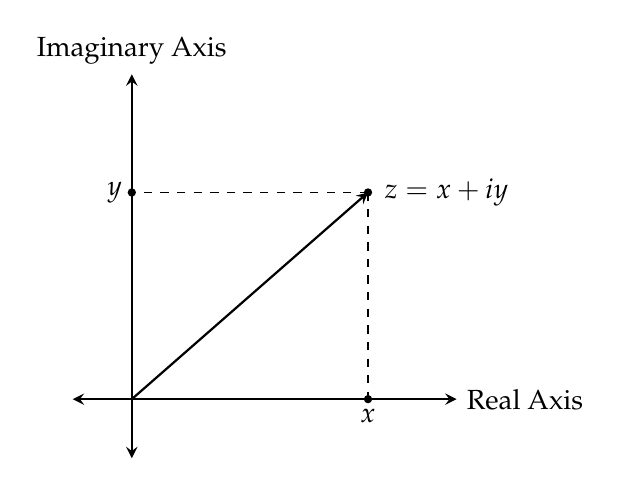
\begin{tikzpicture}[scale=0.75]
    \draw[<->,thick] (-1,0)--(5.5,0) node[right]{Real Axis};
	\draw[<->,thick] (0,-1)--(0,5.5) node[above]{Imaginary Axis};
	\draw[dashed] (4,3.5)--(0,3.5);
	\draw[dashed] (4,3.5)--(4,0);
    \fill (4,3.5) circle (2pt) node[right]{\ $z = x+iy$};
    \fill (0,3.5) circle (2pt) node[left]{$y$};
    \fill (4,0) circle (2pt) node[below]{$x$};
    \draw[->,>=stealth,thick] (0,0) -- (4,3.5);
  \end{tikzpicture}\]
Geometrically, addition of complex numbers is just the addition of the corresponding vectors in the euclidean plane. We will soon see a geometric interpretation of multiplication.

\[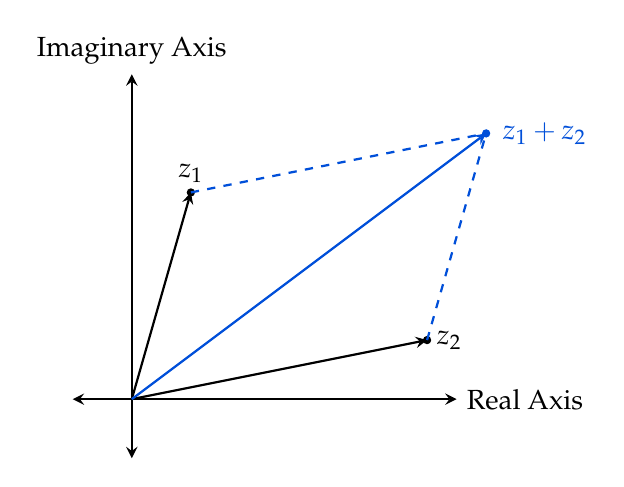
\begin{tikzpicture}[scale=0.75]
    \draw[<->,thick] (-1,0)--(5.5,0) node[right]{Real Axis};
	\draw[<->,thick] (0,-1)--(0,5.5) node[above]{Imaginary Axis};
    \fill[newblue] (6,4.5) circle (2pt) node[right]{\ $z_1 + z_2$};
    \fill (1,3.5) circle (2pt) node[above]{$z_1$};
    \fill (5,1) circle (2pt) node[right]{$z_2$};
    \draw[->,>=stealth,thick] (0,0) -- (1,3.5);
    \draw[->,>=stealth,thick] (0,0) -- (5,1);
	\draw[thick,dashed,newblue] (1,3.5)--(6,4.5);
	\draw[thick,dashed,newblue] (5,1)--(6,4.5);
    \draw[->,>=stealth,thick,newblue] (0,0) -- (6,4.5);
  \end{tikzpicture}\]

\medskip
 
\begin{definition}[Modulus]\label{cmplxnorm}
The \cdef{modulus} (or \cdef{absolute\ value}) of a complex number $z = x + iy$, denoted $\abs{z}$, is the length of the vector $(x,y)$, or equivalently its distance from the origin; namely
\[\abs{z} \coloneqq \sqrt{(\Re z)^2 + (\Im z)^2} = \sqrt{x^2 + y^2} = \norm{(x,y)}\]
Notice that this extends the usual absolute value of real numbers, as the modulus of a real number is its absolute value.\\[0.5em]
We can then immediately derive a useful inequality,
\[\abs{z}^2 = (\Re z)^2 + (\Im z)^2 \geq (\Re z)^2,\  (\Im z)^2,\]
giving us \[\Re z \leq \abs{\Re z} \leq \abs{z}\quad \text{and} \quad \Im z \leq \abs{\Im z} \leq \abs{z}.\]
\end{definition}

\medskip

\begin{definition}[Distance]
The \cdef{distance} between two complex numbers $z_1$ and $z_2$ is \[\abs{z_1 - z_2} = \norm{(x_1,y_1) - (x_2,y_2)} = \norm{(x_1 - x_2,y_1 - y_2)}\]
That is, it's the euclidean distance between the vectors representing these complex numbers. 
\end{definition}

\medskip

\begin{discussion}\label{firstdomain}
The absolute value can be used to define various important subsets of $\cc$.
\begin{itemize}[itemsep=1em]
\item[(1)]
\begin{itemize}[itemsep=1em]
\item[$\bullet$] The \emph{circle of radius $R>0$ centered at $z_0$} is the set
\[C_R(z_0) = \setp{z\in \cc}{\abs{z-z_0}=R}\]
\item[$\bullet$] The \emph{open disk (or ball) of radius $R>0$ centered at $z_0$} is the set
\[D_R(z_0) = \setp{z\in \cc}{\abs{z-z_0}< R}\]\\[-1em]
\[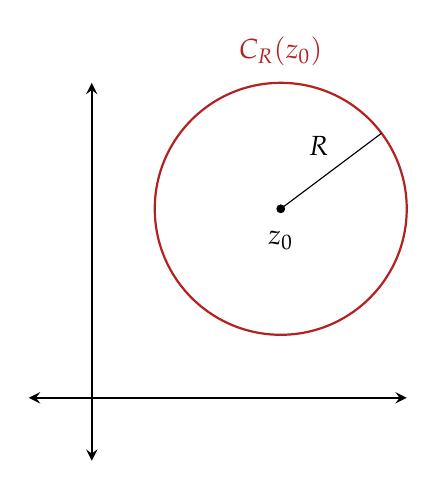
\begin{tikzpicture}[scale=0.8]
    \draw[<->,thick] (-1,0)--(5,0);
	\draw[<->,thick] (0,-1)--(0,5);
    \draw[thick,firebrick](3,3) circle (2);
    \draw[](3,3)--(4.6,4.2);
    \fill (3,3) circle (2pt);
    \node[] at (3,2.5) {$z_0$};
    \node[] at (3,5.5) {\color{firebrick}$C_R(z_0)$};
    \node[] at (3.6,4) {$R$};
  \end{tikzpicture}
  \qquad \qquad \qquad
  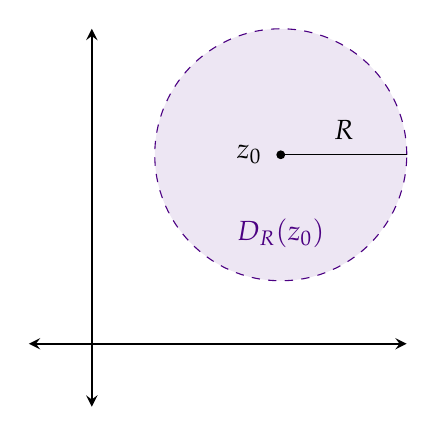
\begin{tikzpicture}[scale=0.8]
    \draw[<->,thick] (-1,0)--(5,0);
	\draw[<->,thick] (0,-1)--(0,5);
	\filldraw[indigo,fill opacity=1/10,dashed](3,3) circle (2);
    \draw[](3,3)--(5,3);
    \fill (3,3) circle (2pt);
    \node[] at (2.5,3) {$z_0$};
    \node[] at (3,1.75) {\color{indigo}$D_R(z_0)$};
    \node[] at (4,3.4) {$R$};
  \end{tikzpicture}\]
\item[$\bullet$] The \emph{closed disk (or ball) of radius $R>0$ centered at $z_0$} is the set
\begin{align*}
\overline{D}_R(z_0) &= \setp{z\in \cc}{\abs{z-z_0} \leq R} = D_R(z_0) \cup C_R(z_0).
\end{align*}
\end{itemize}
\item[(2)] The \emph{(open) annulus of inner radius $r>0$ and outer radius $R>0$ centered at $z_0$} is the set
\[A_{r,R}(z_0) = \setp{z\in \cc}{r < \abs{z-z_0}<R}\]\\[-1em]
\[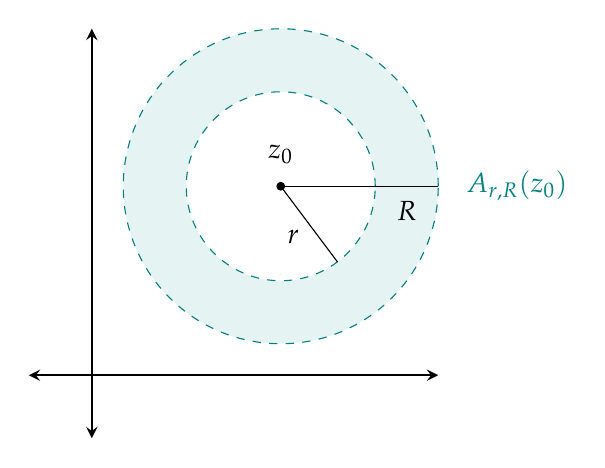
\begin{tikzpicture}[scale=0.8]
    \draw[<->,thick] (-1,0)--(5.5,0);
	\draw[<->,thick] (0,-1)--(0,5.5);
	\filldraw[teal,fill opacity=1/10,dashed](3,3) circle (2.5);
	\fill[white](3,3) circle (1.5);
    \draw[teal,dashed](3,3) circle (1.5);
    \draw[](3,3)--(5.5,3);
    \draw[](3,3)--(3.9,1.8);
    \fill (3,3) circle (2pt);
    \node[] at (3,3.5) {$z_0$};
    \node[] at (6.75,3) {\color{teal}$A_{r,R}(z_0)$};
    \node[] at (5,2.6) {$R$};
    \node[] at (3.2,2.2) {$r$};
  \end{tikzpicture}\]
\end{itemize}
\end{discussion}

%\bigskip

\begin{proposition}[Triangle Inequalities]\label{triangleineq}
For all $z_1,z_2 \in \cc$, the following inequalities hold.
\begin{itemize}
\item[(1)] $\abs{z_1 + z_2} \leq \abs{z_1} + \abs{z_2}$.
\item[(2)] $\abs{z_1 \pm z_2} \geq \abs{\abs{z_1} - \abs{z_2}}$. We sometimes refer to this inequality as the \cdef{reverse\ triangle\ inequality}.
\end{itemize}
\end{proposition}
\begin{proof}
\[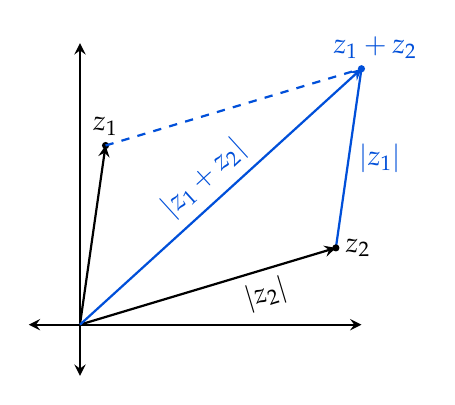
\begin{tikzpicture}[scale=0.65]
    \draw[<->,thick] (-1,0)--(5.5,0);
	\draw[<->,thick] (0,-1)--(0,5.5);
    \fill[newblue] (5.5,5) circle (2pt) node[above]{\quad $z_1 + z_2$};
    \fill (0.5,3.5) circle (2pt) node[above]{$z_1$};
    \draw[->,>=stealth,thick] (0,0) -- (0.5,3.5);
    \draw[->,>=stealth,thick] (0,0) -- (5,1.5) node [pos=0.7, below,sloped] {$\abs{z_2}$};
	\draw[thick,dashed,newblue] (0.5,3.5)--(5.5,5);
	\draw[thick,newblue] (5,1.5)--(5.5,5) node [midway, right] {$\abs{z_1}$};
    \fill (5,1.5) circle (2pt) node[right]{$z_2$};
    \draw[->,>=stealth,thick,newblue] (0,0) -- (5.5,5) node [midway, above,sloped] {$\abs{z_1 + z_2}$};
  \end{tikzpicture}\]
\begin{itemize}
\item[(1)] A standard fact about triangles.
\item[(2)] We first assume that $\abs{z_1} \geq \abs{z_2}$. Then, $\abs{\abs{z_1} - \abs{z_2}} = \abs{z_1} - \abs{z_2}$. Now, note that
\begin{align*}
\abs{z_1} - \abs{z_2} &= \abs{z_1 \pm z_2 \mp z_2} - \abs{z_2}\\[0.5em]
 &\leq \abs{z_1 \pm z_2} + \abs{\mp z_2} - \abs{z_2},\ \text{triangle inequality}\\[0.5em]
 &= \abs{z_1 \pm z_2} + \abs{z_2} - \abs{z_2}\\[0.5em]
 &= \abs{z_1 \pm z_2}
\end{align*}
If we instead assume $\abs{z_2} \geq \abs{z_1}$, then we do the same computation with the roles of $z_1$ and $z_2$ switched.
\end{itemize}
\vspace*{-\baselineskip}
\end{proof}

\medskip


\begin{proposition}[Modulus is Multiplicative]\label{normmult}
\lecmargin{3}
For all $z,w \in \cc$ and positive integers $n$, 
\begin{multicols}{2}
\begin{itemize}
\item[(1)] $\abs{zw} = \abs{z}\abs{w}$.
\item[(2)] $\abs{z^n} = \abs{z}^n$.
\end{itemize}
\end{multicols}
\end{proposition}
\begin{proof}\hfill
\begin{itemize}
\item[(1)] Left as Problem \ref{prob 2.1a}. One proves these directly by showing that the left hand side matches the right hand side.
\item[(2)] The proof of this is by induction. $n = 1$ is a tautology, and $n = 2$ is (1) in the case $w = z$. Assume the statement is true for $n = k$, that is $\abs{z^k} = \abs{z}^k$. Then, for $n = k + 1$
\begin{align*}
|z^{k+1}| = |z^k\cdot z| &= |z^k|\abs{z},\quad \text{using (1)}\\[0.5em]
&= \abs{z}^k\abs{z},\quad \text{using the induction hypothesis}\\[0.5em]
&= \abs{z}^{k+1}
\end{align*}
Therefore we have the result by the principle of mathematical induction.
\end{itemize}
\vspace*{-\baselineskip}
\end{proof}

\medskip

\begin{definition}[Complex Conjugation]
Given a complex number $z = x + iy$, its \cdef{(complex)\ conjugate}, denoted $\overline{z}$, is
\[\overline{z} \coloneqq x - iy\]
Geometrically, $\overline{z}$ is the reflection of $z$ about the real axis. 
\[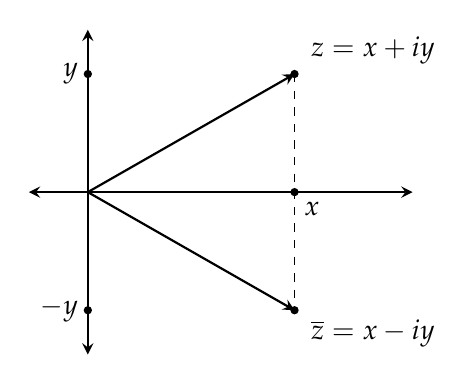
\begin{tikzpicture}[scale=0.75]
    \draw[<->,thick] (-1,0)--(5.5,0);
	\draw[<->,thick] (0,-2.75)--(0,2.75);
    \fill (3.5,2) circle (2pt) node[above right]{\ $z = x+iy$};
    \draw[->,>=stealth,thick] (0,0) -- (3.5,2);
    \fill (3.5,-2) circle (2pt) node[below right]{\ $\overline{z} = x-iy$};
    \draw[->,>=stealth,thick] (0,0) -- (3.5,-2);
    \draw[-,dashed] (3.5,2) -- (3.5,-2);
    \fill (3.5,0) circle (2pt) node[below right]{$x$};
    \fill (0,2) circle (2pt) node[left]{$y$};
    \fill (0,-2) circle (2pt) node[left]{$-y$};
  \end{tikzpicture}\]
\end{definition}

\medskip

\begin{proposition}[Properties of Conjugation]\label{conjprop}
For all pairs $z,w \in \cc$, we have
\begin{itemize}
\item[(1)] $\overline{\overline{z}} = z$
\item[(2)] $\abs{\overline{z}} = \abs{z}$
\item[(3)] $\overline{z + w} = \overline{z} + \overline{w}$
\item[(4)] $\overline{zw} = \overline{z}\ \overline{w}$
\item[(5)] $z\overline{z} = \abs{z}^2$
\item[(6)] $\Re z = \dfrac{z + \overline{z}}{2}$ and $\Im z = \dfrac{z - \overline{z}}{2i}$
\item[(7)] $z \in \rr$ if and only if $z = \overline{z}$
\end{itemize}
\end{proposition}
\begin{proof}
(1) -- (3) is clear geometrically. (4), (6) and (7) are left as Problem \ref{prob 2.1}, (7) can be proved using (6) and can also be deduced geometrically. One proves these directly by showing that the left hand side matches the right hand side.
\begin{itemize}
\item[(5)] Let $z = x + iy$, then
\begin{align*}
z\overline{z} &= (x + iy)(x - iy)\\[0.5em]
&= x^2 - ixy + iyx - i^2y^2\\[0.5em]
&= x^2 + y^2 + i(yx - xy) = x^2 + y^2 = \abs{z}^2\\[-1em]
\end{align*}
\end{itemize}
\vspace*{-\baselineskip}
\end{proof}

\medskip

\begin{discussion}
Proposition \ref{conjprop} (5) gives us a nice formula for $z^{-1}$ for $z\in \cc^*$. For such a $z$, we have $z\overline{z} = \abs{z}^2$, which gives us
\[z^{-1} = z^{-1}\cdot \frac{z\overline{z}}{\abs{z}^2} = \frac{\overline{z}}{\abs{z}^2}\]
This tells us that $z^{-1}$ is just a scaled $\overline{z}$, which means, geometrically speaking, $z^{-1}$ lies on the line passing through the origin and $\overline{z}$.
\end{discussion}

\medskip

\lecmargin{4}
Recall that every non-zero point $(x,y) \in \rr^2$ can be re-written in polar coordinates $(r,\theta)$ as
\[x = r\cos\theta \quad \text{and} \quad y = r\sin\theta\]
This suggests the following definition.
\begin{definition}[Polar Form]
If $(r,\theta)$ are polar coordinates for a non-zero $(x,y)$, then the \cdef{polar\ form} of a non-zero complex number $z = x + iy$ is
\[z = r(\cos\theta + i\sin\theta)\]
We sometimes abbreviate $\cos\theta + i\sin\theta$ as $\cis\theta$, so $z = r\cis\theta$.\\
\\
Evidently, $(r,\theta)$ are related to $(x,y)$ by the equations
\[\abs{z} = r \quad \text{and} \quad \cos\theta = \frac{x}{r} = \frac{x}{\sqrt{x^2 + y^2}},\ \sin\theta = \frac{y}{r} = \frac{y}{\sqrt{x^2 + y^2}},\ \text{so } \tan\theta = \frac{y}{x}\]
We have to be careful and take into account which quadrant $(x,y)$ belongs to, if we think of $\theta$ with respect to its formulation using $\tan$.
\[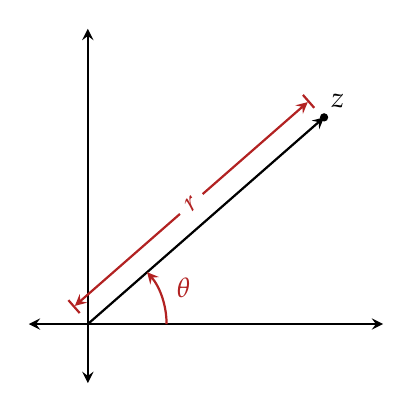
\begin{tikzpicture}[scale=0.75]
    \draw[<->,thick] (-1,0)--(5,0);
	\draw[<->,thick] (0,-1)--(0,5);
	\fill (4,3.5) circle (2pt) node[above]{\quad $z$};
    \draw[->,>=stealth,thick] (0,0) -- (4,3.5);
    \draw[|<->|,>=stealth,thick,firebrick] (-0.2478,0.2832) -- (3.752,3.783) node [fill=white, midway, sloped] {$r$};
    \draw
    (4,3.5) coordinate (a)
    -- (0,0) coordinate (b)
    -- (0.5,0) coordinate (c)
    pic["$\color{firebrick}\theta$", ->,>=stealth,thick, draw=firebrick, angle eccentricity=1.3, angle radius=1cm]
    {angle=c--b--a};
  \end{tikzpicture}\]
Since $\sin$ and $\cos$ are periodic functions, $\theta$ is not unique (you can replace $\theta$ with $\theta + 2\pi$). Each possible value of $\theta$ is called an \cdef{argument\ of} {\color{darkred}$z$}, and the set of all such $\theta$ is denoted as $\arg z$. That is, if $\theta_0$ is one solution of $\tan\theta = y/x$, then
\[\arg z = \setp{\theta_0 + 2k\pi}{k \in \zz}\]
The polar form, specifically $\theta$ is unique, as soon as we specify bounds on $\theta$. The unique argument in the interval $(-\pi,\pi]$ is called the \cdef{principal\ argument} denoted $\parg z$. Precisely speaking,
\begin{definition}\label{princ-arg}
For $z = x + iy$, we have
\[\parg z = \begin{cases}\arctan(y/x) & \text{if $x > 0$\quad \emph{\small(quadrants I \& IV)}}\\[0.5em]
\arctan(y/x) + \pi & \text{if $x < 0$ and $y > 0$\quad \emph{\small(quadrant II)}}\\[0.5em]
\arctan(y/x) - \pi & \text{if $x < 0$ and $y < 0$\quad \emph{\small(quadrant III)}}
 \end{cases}\]
\end{definition}
Notice that we can then write
\[\arg z = \setp{\parg z + 2k\pi}{k \in \zz}\]
\end{definition}

\medskip

\begin{definition}[Euler's Formula]\label{eulerform}
$e^{i\theta} \coloneqq \cis\theta = \cos\theta + i\sin\theta$. Therefore $\abs{e^{i\theta}} = 1$.
\end{definition}
\begin{proof}[Remark on Definition \ref{eulerform}]\renewcommand{\qedsymbol}{}
This is for now a stopgap, defining $e^{i\theta}$ in this way. In a few weeks, we'll see that this is truly an equality of holomorphic functions. Euler deduced this by looking at the Taylor series expansion of these functions. We haven't built or discussed enough machinery to give this reasoning a solid foundation yet. 
\end{proof}

\medskip

Using Euler's formula, one can write the polar form of a non-zero complex number, even more succinctly in its \cdef{exponential\ form}
\[z = re^{i\theta}\]
\begin{example}\hfill
\begin{itemize}[itemsep=1em]
\item[(1)] Exponential form of $1 + i$, 
\[\abs{1 + i} = \sqrt{1^2 + 1^2} = \sqrt{2}\quad \text{and} \quad \parg z = \arctan(1) = \frac{\pi}{4}\]
So, $1 + i = \sqrt{2}e^{i\pi/4}$.
\[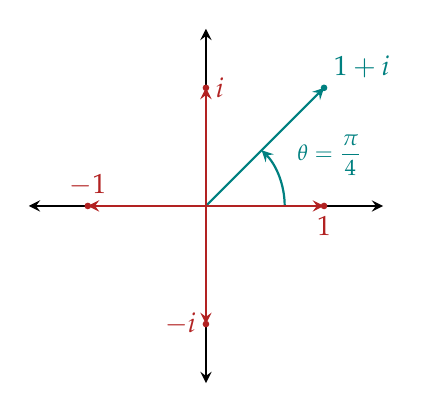
\begin{tikzpicture}[scale=1.5]
    \draw[<-,thick] (-1.5,0)--(-1,0);
	\draw[->,thick] (0,1)--(0,1.5);
	\draw[->,thick] (1,0)--(1.5,0);
	\draw[<-,thick] (0,-1.5)--(0,-1);
	\fill[teal] (1,1) circle (0.8pt) node[above right]{\color{teal}$1+i$};
    \node (a) at (1,1) {};
    \node (b) at (0,0) {};
    \node (c) at (0.5,0) {};
    \draw pic["{\footnotesize$\color{teal}\theta = \dfrac{\pi}{4}$}", ->,>=stealth,thick, draw=teal, angle eccentricity=1.7, angle radius=1cm] {angle=c--b--a};
  \draw[->,>=stealth,teal,thick] (0,0) -- (1,1);
  \draw[->,>=stealth,firebrick,thick] (0,0) -- (1,0);
  \fill[firebrick] (1,0) circle (0.8pt) node[below]{\color{firebrick}$1$};
  \draw[->,>=stealth,firebrick,thick] (0,0) -- (0,1);
  \fill[firebrick] (0,1) circle (0.8pt) node[right]{\color{firebrick}$i$};
  \draw[->,>=stealth,firebrick,thick] (0,0) -- (-1,0);
  \fill[firebrick] (-1,0) circle (0.8pt) node[above]{\color{firebrick}$-1$};
  \draw[->,>=stealth,firebrick,thick] (0,0) -- (0,-1);
  \fill[firebrick] (0,-1) circle (0.8pt) node[left]{\color{firebrick}$-i$};
    \end{tikzpicture}\]
\item[(2)] Note that
\[1 = e^{i0} = e^{i2n\pi}\ \text{for any $n \in \zz$},\qquad i = e^{i\pi/2},\qquad -1 = e^{i\pi} = e^{i(2n+1)\pi}\ \text{for any $n \in \zz$}\]
One could write $-i = e^{i3\pi/2}$ but $3\pi/2 \neq \parg(-i)$; instead we should write $-i = e^{-i\pi/2}$.

\item[(3)] The circle $C_R(z_0)$ has a nice parametrisation 
\[C_R(z_0) = \{z = z_0 + Re^{i\theta}\ :\ 0 \leq \theta < 2\pi\}\]\\[-1.5em]
\[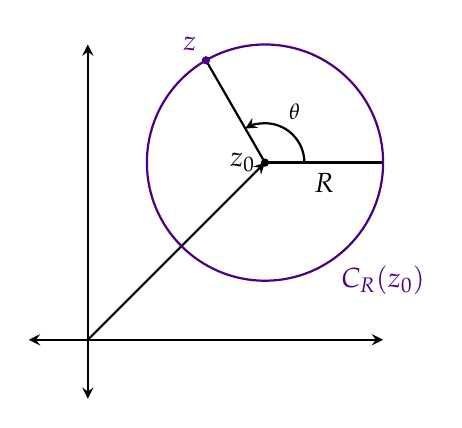
\begin{tikzpicture}[scale=0.75]
    \draw[<->,thick] (-1,0)--(5,0);
	\draw[<->,thick] (0,-1)--(0,5);
	\draw[->,>=stealth,thick] (0,0) -- (3,3);
    \draw[thick,indigo](3,3) circle (2);
    \draw[thick](3,3)--(5,3) node[midway, below]{$R$};
    \fill (3,3) circle (2pt);
    \node[left] at (3,3) {$z_0$};
    \draw[thick](3,3)--(2,4.732);
    \fill[indigo] (2,4.732) circle (2pt) node[above left]{$z$};
    \node (a) at (2,4.732) {};
    \node (b) at (3,3) {};
    \node (c) at (5,3) {};
    \draw pic["{\footnotesize$\theta$}", ->,>=stealth,thick,draw, angle eccentricity=1.5, angle radius=0.5cm] {angle=c--b--a};
    \node[] at (5,1) {\color{indigo}$C_R(z_0)$};
  \end{tikzpicture}\]
\end{itemize}
\vspace*{-\baselineskip}
\end{example}

\medskip

\begin{example}[in-class]
Write the exponential form of $z = 1 - i$.
\end{example}
\begin{proof}[Answer]
As a point on the plane, since $\Re z > 0$ and $\Im z < 0$, the complex number $z = 1 - i$ lies in the fourth quadrant. Thus, 
\begin{align*}
r = \abs{z} &= \sqrt{(1)^2 + (-1)^2} = \sqrt{2}\\[0.5em]
\parg z &= \arctan(-1) = -\frac{\pi}{4}
\end{align*}
Thus, $1 - i = \sqrt{2}e^{-i \pi/4}$. 
\end{proof}

\medskip

\begin{proposition}[Properties of Exponential Form]\label{propeuler}
Let $z = re^{i\theta}$ and $w = se^{i\phi}$ be non-zero complex numbers. Then
\begin{itemize}
\item[(1)] $zw = rs\  e^{i(\theta + \phi)}$
\item[(2)] $z^{-1} = (1/r) e^{-i\theta}$
\item[(3)] $z^n = r^n e^{in\theta}$, for any $n \in \zz$
\item[(4)] $\overline{z} = re^{-i\theta}$
\item[(5)] $z/w = (r/s)e^{i(\theta - \phi)}$
\end{itemize}
\end{proposition}
\begin{proof}\hfill
\begin{itemize}
\item[(1)] Note that
\begin{align*}
zw = (re^{i\theta})(se^{i\phi})&= rs(\cos\theta + i\sin\theta)(\cos\phi + i\sin\phi)\\[0.5em]
&= rs((\cos\theta\cos\phi - \sin\theta\sin\phi) + i(\cos\theta\sin\phi + \sin\theta\cos\phi))\\[0.5em]
&= rs(\cos(\theta + \phi) + i\sin(\theta + \phi))\\[0.5em]
&= rs\  e^{i(\theta + \phi)}
\end{align*}
\item[(2)] It suffices to show that $(re^{i\theta})((1/r) e^{-i\theta}) = 1$, for which we use (1).
\item[(3)] We first prove this result for $n \geq 0$, the result is clear for $n = 0$ and $n = 1$. Assume the result is true for $n = k$, that is $z^k = r^k e^{ik\theta}$. Then, for $n = k+1$
\begin{align*}
z^{k+1} &= z^kz\\[0.5em]
&= (r^k e^{ik\theta})(re^{i\theta})\ \text{using the induction hypothesis}\\[0.5em]
&= r^{k+1} e^{ik\theta+\theta}\ \text{by (1)}\\[0.5em]
&= r^{k+1} e^{i(k+1)\theta}
\end{align*}
Therefore we have the result by the principle of mathematical induction.\\[0.5em]
Suppose $n<0$ instead, then write $n = -m$ for a positive $m>0$. Now, we can apply the first case to $z^n \coloneqq (z^{-1})^m$ to get our result.
\item[(4)] Using $z\overline{z} = \abs{z}^2 = r^2$, we get that $\overline{z} = r^2z^{-1}$, and the result follows from (2).
\item[(5)] Recall $z/w = zw^{-1}$, and the result follows from (2) and (1).
\end{itemize}
\vspace*{-\baselineskip}
\end{proof}

\medskip

\begin{discussion}
Proposition \ref{propeuler} (1) gives us a nice geometric interpretation of complex multiplication. If $z = re^{i\theta}$ and $w = se^{i\phi}$, then $zw = rs\  e^{i(\theta + \phi)}$. This can be interpreted as saying that $zw$ is obtained from $w$ by scaling $w$ by $\abs{z} = r$ and rotating $w$ by an angle of $\parg z$ (or vice versa).
\[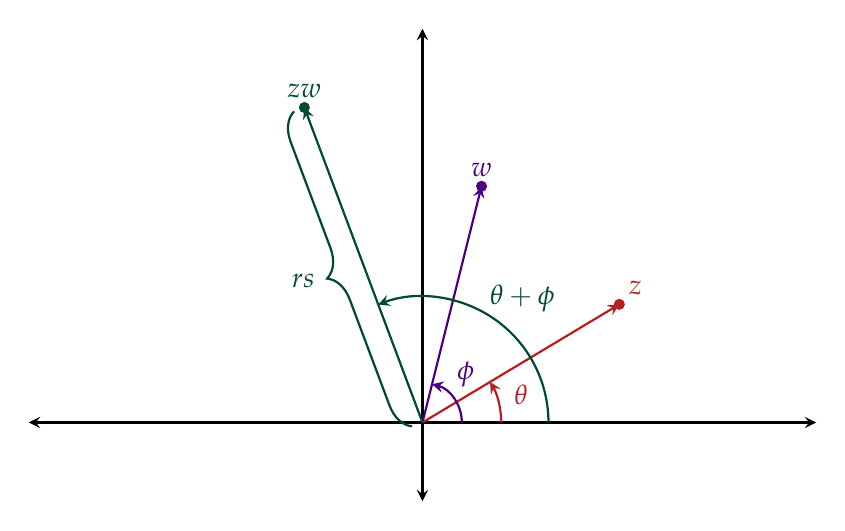
\begin{tikzpicture}
    \draw[<->,thick] (-5,0)--(5,0);
	\draw[<->,thick] (0,-1)--(0,5);
	\fill[firebrick] (2.5,1.5) circle (2pt) node[above right]{$z$};
    \draw[->,>=stealth,thick,firebrick] (0,0) -- (2.5,1.5);
    \node (a) at (2.5,1.5) {};
    \node (b) at (0,0) {};
    \node (c) at (0.2,0) {};
    \draw pic["$\color{firebrick}\theta$", ->,>=stealth,thick, draw=firebrick, angle eccentricity=1.3, angle radius=1cm] {angle=c--b--a};
    
	\fill[indigo] (0.75,3) circle (2pt) node[above]{$w$};
    \draw[->,>=stealth,thick,indigo] (0,0) -- (0.75,3);
    \node (a) at (0.75,3) {};
    \node (b) at (0,0) {};
    \node (c) at (0.2,0) {};
    \draw pic["$\color{indigo}\phi$",left, ->,>=stealth,thick, draw=indigo, angle eccentricity=2, angle radius=0.5cm] {angle=c--b--a};

	\fill[forest] (-1.5,4) circle (2pt) node[above]{$zw$};
    \draw[->,>=stealth,thick,forest] (0,0) -- (-1.5,4);
    \node (a) at (-1.5,4) {};
    \node (b) at (0,0) {};
    \node (c) at (0.2,0) {};
    \draw pic["\quad$\color{forest}\theta + \phi$", ->,>=stealth,thick, draw=forest, angle eccentricity=1.2, angle radius=1.6cm] {angle=c--b--a};
%    \draw[|<->|,>=stealth,thick] (-2.158,3.754) -- (-0.6575,-0.247) node [fill=white, midway, sloped] {$\abs{z}\abs{w}$};
    \draw [decorate,decoration={brace,amplitude=10pt,mirror,raise=4pt},yshift=0pt,thick,forest]
(-1.5,4) -- (0,0) node [black,midway,left,xshift=-0.4cm,yshift=-0.2cm] {$\color{forest}rs\ $};
  \end{tikzpicture}\]

\medskip

\begin{example}
Let's use Proposition \ref{propeuler} to compute $(1+i)^{2023}$, then
\begin{align*}
(1 + i)^{2023} &= (\sqrt{2} e^{i\pi/4})^{2023}\\[0.5em]
 &= (\sqrt{2})^{2023}(e^{i\pi/4})^{2023}\\[0.5em]
 &= (\sqrt{2})^{2022}\sqrt{2}(e^{i\pi/4})^{2024}e^{-i\pi/4}\\[0.5em]
 &= 2^{1011}\sqrt{2}(e^{i506\pi})e^{-i\pi/4}\\[0.5em]
&= 2^{1011}\sqrt{2}e^{-i\pi/4}\\[0.5em]
&= 2^{1011}(1-i)
\end{align*}
\end{example}

\medskip

\begin{example}
Compute $(1+i\sqrt{3})^{101}$.
\end{example}
\begin{proof}[Answer]
We will first compute the exponential form of our complex number. Note that \[|1 + i\sqrt{3}| = \sqrt{1^2 + (\sqrt{3})^2} = \sqrt{4} = 2,\] and since $1 + i\sqrt{3}$ lies in the first quadrant of the complex plane
\[\parg z = \arctan(\sqrt{3}) = \frac{\pi}{3}\]
Therefore
\[1+i\sqrt{3} = 2e^{i\pi/3}\]
and so
\begin{align*}
(1+i\sqrt{3})^{101} &= (2e^{i\pi/3})^{101}\\[0.5em]
 &= (2e^{i\pi/3})^{99}(2e^{i\pi/3})^{2}\\[0.5em]
 &= 2^{99}e^{i33\pi}(1+i\sqrt{3})^{2}\\[0.5em]
 &= -2^{99}(1-3 +2i\sqrt{3}),\quad \text{since $33$ is odd}\\[0.5em]
 &= -2^{99}(-2 +2i\sqrt{3})\\[0.5em]
 &= 2^{100}(1- i\sqrt{3})
\end{align*}
\end{proof}

\medskip

\lecmargin{5}
A few more interesting consequences of Proposition \ref{propeuler} are
\begin{itemize}
\item[(1)] The \emph{unit circle} \[S^1 = \setp{z\in \cc}{\abs{z} = 1} = \{e^{i\theta}\ :\ \theta \in \rr\}\] is closed under multiplication. It's in fact an abelian group, usually denoted $U(1)$.
\item[(2)] \emph{De Moivre's Theorem}. From Proposition \ref{propeuler} (4) applied to $z = e^{i\theta}$ we get
\[(\cos\theta + i\sin\theta)^n = (\cos n\theta + i\sin n\theta)\]
\end{itemize}
\vspace*{-\baselineskip}
\end{discussion}

\medskip

\begin{proposition}[Arguments of Products]\label{prodarg}
Let $z,w$ be non-zero complex numbers, then
\begin{itemize}
\item[(1)] $\arg (zw) = \arg z + \arg w$
\item[(2)] $\arg w^{-1} = -\arg w$
\end{itemize}
\emph{Note that this is \emph{not} saying $\parg(zw) = \parg z + \parg w$, this is actually not true, we're claiming an equality of sets. (1) and (2) together give us $\arg (z/w) = \arg z - \arg w$.}
\end{proposition}
\begin{proof}\hfill
\begin{itemize}
\item[(1)] Consider $\theta \in \arg z$ and $\phi \in \arg w$, so $z = re^{i\theta}$ and $w = se^{i\phi}$. By Proposition \ref{propeuler} (1), we have $zw = rs\ e^{i(\theta + \phi)}$ and therefore $\theta + \phi \in \arg(zw)$. Hence $\arg z + \arg w \subseteq \arg(z + w)$.\\[0.5em]
Consider $\psi \in \arg(z+w)$, and some $\theta \in \arg z$ then we claim that $\psi - \theta \in \arg w$. We have $rs\ e^{i\psi} = zw = re^{i\theta}w$, then by Proposition \ref{propeuler} (5), we get $w = sr^{i(\psi - \theta)}$. Hence $\psi - \theta \in \arg w$, and since $\psi = \theta + (\psi - \theta) \in \arg z + \arg w$, we have $\arg(z+w) \subseteq \arg z + \arg w$.\\[0.5em]
Therefore $\arg (zw) = \arg z + \arg w$.
\item[(2)] Consider $\theta \in \arg z$, so $z = re^{i\theta}$. By Proposition \ref{propeuler} (2), we have $z^{-1} = (1/r)e^{i(-\theta)}$ and therefore $-\theta \in \arg w^{-1}$. Hence $-\arg w \subseteq \arg w^{-1}$.\\[0.5em]
Note that $w = (w^{-1})^{-1}$, applying the above result to $w^{-1}$ gets us $-\arg w^{-1} \subseteq \arg (w^{-1})^{-1} = \arg w$ and so $\arg w^{-1} \subseteq - \arg w$.\\[0.5em]
Therefore $\arg w^{-1} = -\arg w$.
\end{itemize}
\vspace*{-\baselineskip}
\end{proof}

\medskip

\begin{remark}
For a complex number, $\arg z$ is a set of all possible $\theta$'s such that we can write $z = \abs{z}e^{i\theta}$, as you know. Therefore, we will abuse notation by sometimes calling any $\theta \in \arg z$ as an argument of $z$, and sometimes also writing $z = \abs{z}e^{i\arg z}$. That is, we are not, or are careless about, distinguishing the set $\arg z$ and its element when we can be agnostic about the choice of $\theta$; for example, the polar form of a complex number. It will be clear when we choose to care about out choice, it will be evident because we'll be then forcing $\theta$ to lie in an interval of length $2\pi$; for example, the principal argument $-\pi < \parg z \leq \pi$.
\end{remark}

\medskip

\begin{example}\hfill
\begin{itemize}
\item[(1)] The principal argument of $z = (\sqrt{3} - i)^6$. We first note that $\parg(\sqrt{3} - i) = -\pi/6$. By Proposition \ref{prodarg} (1), applied inductively, we have
\begin{align*}
\arg (\sqrt{3} - i)^6 &= \underbrace{\arg(\sqrt{3} - i) + \cdots + \arg(\sqrt{3} - i)}_{\text{$6$ times}} = \setp{-\pi + 2k\pi}{k \in \zz}
\end{align*}
Then $\parg(\sqrt{3} - i)^6$ is the element in the set above in the interval $(-\pi,\pi]$ which is $\pi$.
\item[(2)] As mentioned previously, we can't just replace $\arg$ with $\parg$ in the statement of Proposition \ref{prodarg} (1). Here's a simple example: let $z = w = -1$, then $\parg z = \parg w = \pi$ and $\parg zw = \parg 1 = 0$ but $0 \neq 2\pi = \parg z + \parg w$.
\item[(3)] Note that $\arg z + \arg z \neq 2\arg z$.
\end{itemize}
\vspace*{-\baselineskip}
\end{example}

\bigskip

\subsection{Roots of Complex Numbers}
%\begin{mdframed}
%\begin{center}
%{\Large Roots of Complex Numbers}
%\end{center}
%\end{mdframed}

\begin{lemma}\label{polareq}
Two non-zero complex numbers $z,w$ are equal if and only if $\abs{z} = \abs{w}$ and $\arg z = \arg w$.
\end{lemma}
\begin{proof}
If $\abs{z} = \abs{w}$ and $\arg z = \arg w$, then clearly $z = w$.\\[0.5em]
Suppose $z = w$, then we immediately get $\abs{z} = \abs{w}$. Consider $\theta \in \arg z$ and $\phi \in \arg w$, then we get $e^{i\theta} = e^{i\phi}$ which is equivalent to saying $\cos(\theta - \phi) + i\sin(\theta - \phi) = e^{i(\theta - \phi)} = 1$. This gives us
\[\sin (\theta - \phi) = 0.\]
The solution to this is $\theta - \phi = 2k\pi$ for some $k\in \zz$. This gives us $\arg z = \arg w$.
\end{proof}

\medskip

\begin{definition}[Roots]
\lecmargin{6}
Let $\alpha$ be a non-zero complex number. An \emph{$n^{\text{th}}$ root of $\alpha$} is a solution to the polynomial equation $z^n - \alpha = 0$.\\
\\
The set of all $n^{\text{th}}$ roots of $\alpha$ is denoted by $\alpha^{1/n}$, we reserve the symbol $\sqrt[n]{\ \cdot\ }$ for the unique positive $n^{\text{th}}$ root of a positive real number.
\end{definition}

\medskip

\begin{proposition}[Distinct Roots]\label{distroot}
There are precisely $n$ distinct $n^{\text{th}}$ roots of $\alpha$, namely
\[\beta_k = \sqrt[n]{\abs{\alpha}}\ e^{i\left(\frac{\parg \alpha}{n} + \frac{2k\pi}{n}\right)},\quad k = 0,\ldots,n-1\]
\end{proposition}
\begin{proof}
Let $z = re^{i\theta}$ and $\alpha = \abs{\alpha}e^{i\parg\alpha}$, we solve
\[r^ne^{in\theta} = z^n = \alpha = \abs{\alpha}e^{i\parg\alpha}.\]
By Lemma \ref{polareq}, this equality is true if and only if $r^n = \abs{\alpha}$ and $n\theta = \parg\alpha + 2k\pi$ for some $k \in \zz$. Therefore
\[z = \sqrt[n]{\abs{\alpha}}\ e^{i\left(\frac{\parg \alpha}{n} + \frac{2k\pi}{n}\right)},\quad k \in \zz\]
We obtain distinct $n$ complex numbers for $k = 0,\ldots,n-1$ since they have distinct arguments, and they necessarily give us the $n$ distinct $n^{\text{th}}$ roots of $\alpha$.
\end{proof}

\medskip

\begin{discussion}
With the notation of Proposition \ref{distroot}, the {\color{darkred}$n^{\text{th}}$} \cdef{principal\ root\ of} {\color{darkred}$\alpha$} is
\[\beta_0 = \sqrt[n]{\abs{\alpha}}\ e^{i\frac{\parg \alpha}{n}}\]
If we introduce the notation $\zeta_n = e^{\frac{2\pi i}{n}}$, then
\[\zeta_n^k = e^{\frac{2k\pi i}{n}}\]
According to the proposition, the complex numbers
\[1,\ \zeta_n,\ \zeta_n^2,\ldots,\zeta_n^{n-1}\]
are the distinct solutions to $z^n - 1 = 0$, the {\color{darkred}$n^{\text{th}}$} \cdef{roots\ of\ unity}, making $\zeta_n$ the \cdef{primitive} \emph{$n^{\text{th}}$ root of unity} as it generates all $n^{\text{th}}$ other roots of unity.\\
\\
Then we can write the roots of $\alpha$ in terms of the principal root and the primitive root of unity
\begin{align*}
\beta_k &= \sqrt[n]{\abs{\alpha}}\ e^{i\left(\frac{\parg \alpha}{n} + \frac{2k\pi}{n}\right)}\\[0.5em]
 &= \sqrt[n]{\abs{\alpha}}\ e^{i\frac{\parg \alpha}{n}}e^{\frac{2k\pi i}{n}}  = \beta_0\zeta_n^k
\end{align*}
That is, $\beta_k$'s all lie on the circle of radius $\sqrt[n]{\abs{\alpha}}$ centered at the origin, and all of them are obtained by rotating $\beta_0$ by an angle of $2k\pi/n$. That is, they all lie on the vertices of an inscribed regular $n$-gon.
\[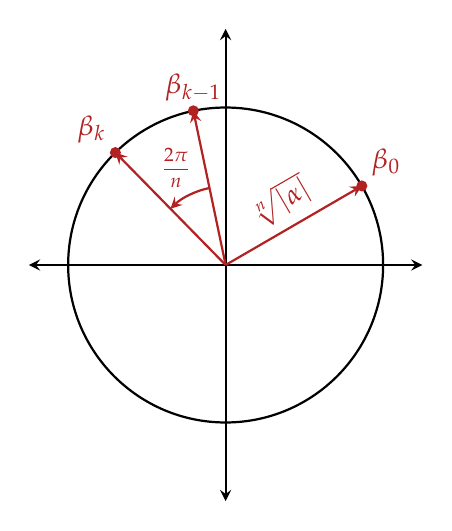
\begin{tikzpicture}
    \draw[<->,thick] (-2.5,0)--(2.5,0);
	\draw[<->,thick] (0,-3)--(0,3);
    \draw[thick](0,0) circle (2);
    \draw[->,>=stealth,thick,firebrick](0,0)--(-0.41,1.958);
    \draw[->,>=stealth,thick,firebrick](0,0)--(-1.4,1.428);
    \fill[firebrick] (-0.41,1.958) circle (2pt) node[above]{\color{firebrick}$\beta_{k-1}$};
    \fill[firebrick] (-1.4,1.428) circle (2pt) node[above left]{\color{firebrick}$\beta_{k}$};
    \node (a) at (-1.4,1.428) {};
    \node (b) at (0,0) {};
    \node (c) at (-0.41,1.958) {};
    \draw[->,>=stealth,thick,firebrick](0,0)--(1.73,1.004) node[midway,above,sloped]{\color{firebrick}$\sqrt[n]{\abs{\alpha}}$};
    \fill[firebrick] (1.73,1.004) circle (2pt) node[above right]{\color{firebrick}$\beta_0$};
    \draw pic["{\scriptsize$\color{firebrick}\ \dfrac{2\pi}{n}$}", ->,>=stealth,thick,draw=firebrick, angle eccentricity=1.4, angle radius=1cm] {angle=c--b--a};
  \end{tikzpicture}\]
\end{discussion}

\medskip

\begin{example}\hfill
\begin{itemize}
\item[(1)] We compute explicitly the $4^{\text{th}}$ roots of $\alpha = -16$. As a negative real number, $\parg(-16) = \pi$, so
\begin{align*}
\beta_k &= \sqrt[4]{16}e^{i\left(\frac{\pi}{4}+\frac{2k\pi}{4}\right)} = 2\ e^{i\frac{\pi}{4}}e^{\frac{ki\pi}{2}}\\[0.5em]
&= 2\ e^{i\frac{\pi}{4}}\left(e^{\frac{i\pi}{2}}\right)^k\\[0.5em]
&= 2\ \left(\cos\frac{\pi}{4} + i\sin\frac{\pi}{4}\right)\left(\cos\frac{\pi}{2} + i\sin\frac{\pi}{2}\right)^k = 2\ \left(\frac{1}{\sqrt{2}} + i\frac{1}{\sqrt{2}}\right)i^k = \sqrt{2}(1 + i)i^k
\end{align*}
Therefore
\[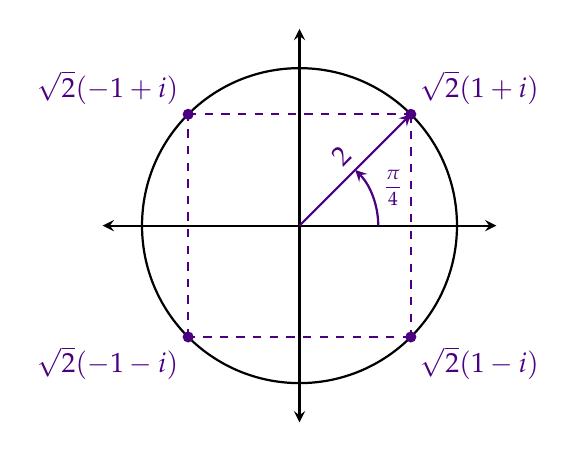
\begin{tikzpicture}
    \draw[<->,thick] (-2.5,0)--(2.5,0);
	\draw[<->,thick] (0,-2.5)--(0,2.5);
    \draw[thick](0,0) circle (2);
    \draw[->,>=stealth,thick,indigo](0,0)--(1.414,1.414) node[above, midway, sloped]{\color{indigo}$2$};
    \draw[thick,indigo,dashed](1.414,1.414)--(1.414,-1.414);
    \draw[thick,indigo,dashed](1.414,-1.414)--(-1.414,-1.414);
    \draw[thick,indigo,dashed](-1.414,-1.414)--(-1.414,1.414);
    \draw[thick,indigo,dashed](-1.414,1.414)--(1.414,1.414);
    \fill[indigo] (1.414,1.414) circle (2pt) node[above right]{\color{indigo}$\sqrt{2}(1 + i)$};
    \fill[indigo] (1.414,-1.414) circle (2pt) node[below right]{\color{indigo}$\sqrt{2}(1 - i)$};
    \fill[indigo] (-1.414,1.414) circle (2pt) node[above left]{\color{indigo}$\sqrt{2}(-1 + i)$};
    \fill[indigo] (-1.414,-1.414) circle (2pt) node[below left]{\color{indigo}$\sqrt{2}(-1 - i)$};
    \node (a) at (1.414,1.414) {};
    \node (b) at (0,0) {};
    \node (c) at (2,0) {};
    \draw pic["{\scriptsize$\color{indigo}\ \dfrac{\pi}{4}$}", ->,>=stealth,thick,draw=indigo, angle eccentricity=1.25, angle radius=1cm] {angle=c--b--a};
  \end{tikzpicture}\]
\[\beta_0 = \sqrt{2}(1 + i),\quad \beta_1 = \sqrt{2}(-1 + i),\quad \beta_2 = \sqrt{2}(-1-i),\quad \beta_3 = \sqrt{2}(1-i)\]
\item[(2)] In the course of the previous example, we have computed the $4^{\text{th}}$ roots of unity, since they are
\[e^{\frac{2ki\pi}{4}} = e^{\frac{ki\pi}{2}},\quad k = 0,1,2,3\]
as $\parg 1 = 0$. Letting $\zeta_4 = e^{i\pi/2} = i$, the $4^{\text{th}}$ roots of unity are $\zeta_4^0,\zeta_4^1,\zeta_4^2,\zeta_4^3$, which are nothing but $\pm 1,\pm i$. Furthermore, note that $i$ is the primitive $4^{\text{th}}$ root of unity. 
\end{itemize}
\end{example}

\medskip

\begin{example}\label{cuberootofunity}
\lecmargin{7}
We compute the $3^{\text{rd}}$ roots of unity, also called the cube roots of unity where we denote $\omega = \zeta_3$, explicitly.
\[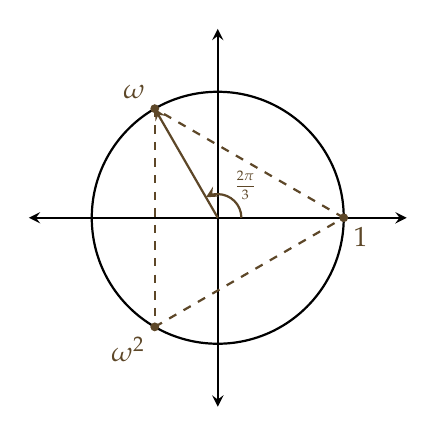
\begin{tikzpicture}[scale=0.8]
    \draw[<->,thick] (-3,0)--(3,0);
	\draw[<->,thick] (0,-3)--(0,3);
    \draw[thick](0,0) circle (2);
    \draw[->,>=stealth,thick,dirt](0,0)--(-1,1.732);
    \draw[thick,dirt,dashed](2,0)--(-1,1.732);
    \draw[thick,dirt,dashed](-1,1.732)--(-1,-1.732);
    \draw[thick,dirt,dashed](-1,-1.732)--(2,0);
    \fill[dirt] (-1,1.732) circle (2pt) node[above left]{\color{dirt}$\omega$};
    \fill[dirt] (-1,-1.732) circle (2pt) node[below left]{\color{dirt}$\omega^2$};
    \fill[dirt] (2,0) circle (2pt) node[below right]{\color{dirt}$1$};
    \node (a) at (-1,1.732) {};
    \node (b) at (0,0) {};
    \node (c) at (2,0) {};
    \draw pic["{\ \ \tiny$\color{dirt}\ \dfrac{2\pi}{3}$}", ->,>=stealth,thick,draw=dirt, angle eccentricity=1.6, angle radius=0.3cm] {angle=c--b--a};
  \end{tikzpicture}\]
Let the primitive root be $\omega = \zeta_3$, then the cube roots of unity are
\[1,\ \omega,\ \omega^2\]
where we have
\begin{align*}
\omega = e^{\frac{2\pi i}{3}} &= \left(\cos\frac{2\pi}{3} + i\sin\frac{2\pi}{3}\right) = -\frac{1}{2}+i\frac{\sqrt{3}}{2}\\[0.5em]
\omega^2 = e^{\frac{4\pi i}{3}} &= \left(\cos\frac{4\pi}{3} + i\sin\frac{4\pi}{3}\right) = -\frac{1}{2}-i\frac{\sqrt{3}}{2}
\end{align*}
\end{example}

\bigskip

\subsection{Basic Topology of $\cc$}
%\begin{mdframed}
%\begin{center}
%{\Large Basic Topology of $\cc$}
%\end{center}
%\end{mdframed}

Our purpose now is to define the kind of subsets of $\cc$ that are suitable for doing complex analysis, namely \emph{non-empty open connected sets}.
\begin{definition}[Open Disks or Neighbourhoods]
Let $\epsilon>0$. Recall the \cdef{open\ disk} (of radius $\epsilon$ centered at $z_0$) is the set
\[D_\epsilon(z_0) = \setp{z\in \cc}{\abs{z - z_0}<\epsilon}.\]
We also refer to such an open disk as an {\color{darkred}$\epsilon$-}\cdef{neighbourhood} or simply a \cdef{neighbourhood}.\\
\\
A \cdef{deleted} (or \cdef{punctured}) \cdef{open\ disk} (or \cdef{neighbourhood}) is a set of the form
\[D_\epsilon(z_0)\setminus\set{z_0} = \setp{z\in \cc}{0 < \abs{z - z_0}<\epsilon}.\]\\[-0.5em]
\[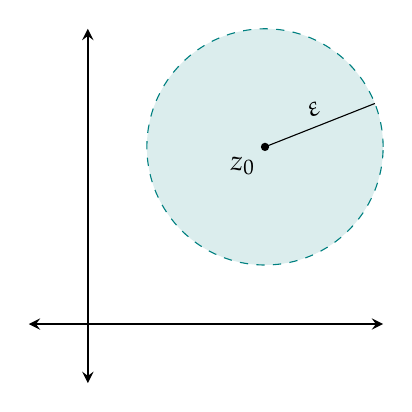
\begin{tikzpicture}[scale=0.75]
    \draw[<->,thick] (-1,0)--(5,0);
	\draw[<->,thick] (0,-1)--(0,5);
	\filldraw[teal,fill opacity=1/7,dashed](3,3) circle (2);
    \draw[](3,3)--(4.86,3.735) node[sloped,midway,above]{$\epsilon$};
    \fill (3,3) circle (2pt) node[below left]{$z_0$};
  \end{tikzpicture}
  \qquad\qquad\qquad
  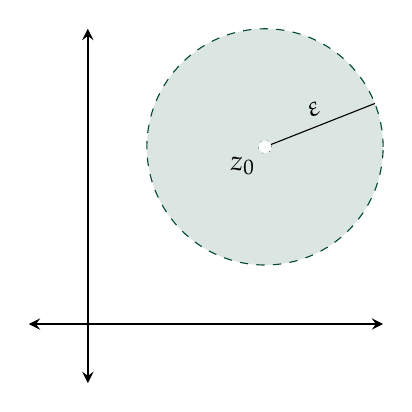
\begin{tikzpicture}[scale=0.75]
    \draw[<->,thick] (-1,0)--(5,0);
	\draw[<->,thick] (0,-1)--(0,5);
	\filldraw[forest,fill opacity=1/7,dashed](3,3) circle (2);
    \draw[forest,dotted](3,3) circle (3pt);    
    \draw[](3,3)--(4.86,3.735) node[sloped,midway,above]{$\epsilon$};
    \fill[white] (3,3) circle (3pt) node[below left]{\color{black}$z_0$};
  \end{tikzpicture}\]
Points belonging to the same $\epsilon$-neighbourhood are considered "close" to each other, in the sense that they are within a distance of $2\epsilon$ from each other.
\end{definition}

\medskip

\begin{definition}[Various kinds of Points]
Consider a $S \subseteq \cc$. 
\begin{itemize}
\item A point $z \in S$ is an \cdef{interior\ point\ of} {\color{darkred}$S$} if there exists an $\epsilon > 0$ such that $D_\epsilon(z) \subseteq S$. 
\item A point $z \notin S$ is an \cdef{exterior\ point\ of} {\color{darkred}$S$} if there exists an $\epsilon > 0$ such that $D_\epsilon(z) \cap S = \emptyset$. 
\item A point $z \in \cc$ is a \cdef{boundary\ point\ of} {\color{darkred}$S$} if it's neither an interior nor an exterior point of $S$. Equivalently, if every neighbourhood of $z$ contains both a point in $S$ and not in $S$.
\item A point $z \in \cc$ is a \cdef{accumulation} (or \cdef{cluster}) \cdef{point\ of} {\color{darkred}$S$} if for every $\epsilon > 0$ we have \[D_\epsilon(z)\setminus\set{z} \cap S \neq \emptyset.\]
\item A point $z \in S$ is an \cdef{isolated\ point\ of} {\color{darkred}$S$} if there exists an $\epsilon > 0$ such that $D_\epsilon(z)\setminus\set{z} \cap S = \emptyset$. Isolated points are examples of boundary point
\end{itemize}
\[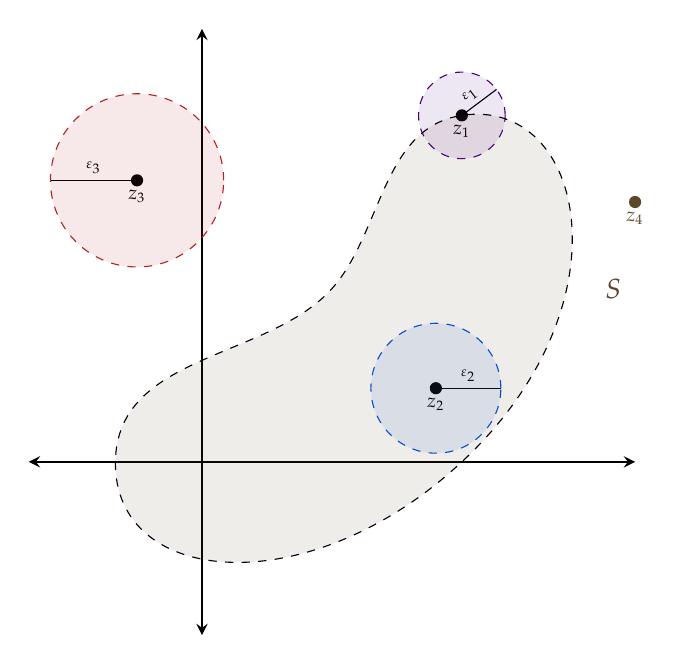
\begin{tikzpicture}[scale=1.1]
    \draw[<->,thick] (-2,0)--(5,0);
	\draw[<->,thick] (0,-2)--(0,5);
    \node[] at (4.75,2) {\color{dirt}$S$};
    
    \fill (3,4) circle (2pt) node[below]{\scriptsize$z_1$};
    \draw[](3,4)--(3.4,4.3) node[sloped,midway,xshift=-1pt,yshift=4pt]{\tiny$\epsilon_1$};
    \filldraw[indigo,fill opacity=1/10,dashed](3,4) circle (0.5);
    
    \fill (2.7,0.85) circle (2pt) node[below]{\scriptsize$z_2$};
    \draw[](2.7,0.85)--(3.45,0.85) node[sloped,midway,above,yshift=-1pt]{\tiny$\epsilon_2$};
    \filldraw[newblue,fill opacity=1/10,dashed](2.7,0.85) circle (0.75);
    
    \fill (-0.75,3.25) circle (2pt) node[below]{\scriptsize$z_3$};
    \draw[](-0.75,3.25)--(-1.75,3.25) node[sloped,midway,above,yshift=-1pt]{\tiny$\epsilon_3$};
    \filldraw[firebrick,fill opacity=1/10,dashed](-0.75,3.25) circle (1);
    
    \path[draw,use Hobby shortcut,closed=true,fill=dirt,fill opacity=1/10,dashed]
(-1,0) .. (3,0) .. (3,4) .. (1.5,2) .. (-1,0);
	\fill[dirt] (5,3) circle (2pt) node[below]{\scriptsize$z_4$};
\end{tikzpicture}\]
Here $z_1$ is a boundary point, $z_2$ an interior point, $z_3$ an exterior point, and $z_4$ is an isolated point (and a boundary point).
\end{definition}

%\medskip

\begin{remark}
The idea is that if we don't move too far from an interior point of $S$ then we remain in $S$; a similar idea holds for an exterior point. But at a boundary point we can make an arbitrarily small move and get to a point inside $S$, and we can also make an arbitrarily small move and get to a point outside $S$. An accumulation point is one where it has other points from $S$ within any arbitrarily small distance, i.e. points "accumulate" near it; an isolated point is the exact opposite.
\end{remark}

\medskip

\begin{definition}[Open and Closed Sets]
Consider a $S \subseteq \cc$.
\begin{itemize}
\item The \cdef{interior\ of} {\color{darkred}$S$} is the set of all interior points of $S$, denoted $S^\circ$.
\item $S$ is said to be \cdef{open} if $S = S^\circ$.
\item The \cdef{boundary\ of} {\color{darkred}$S$} is the set of all boundary points of $S$, denoted $\partial S$.
\item $S$ is said to be \cdef{closed} if $\partial S \subseteq S$. Equivalently, if its complement is open.
\item The \cdef{closure\ of} {\color{darkred}$S$} is the set $S \cup \partial S$, denoted $\overline{S}$.
\end{itemize}
\end{definition}

\medskip

\begin{example}\hfill
\begin{itemize}
\item[(1)] The open disks $D_R(z_0)$ are truly open sets, and the closed disks $\overline{D}_R(z_0)$ are truly closed sets.\\[0.5em]
The closure of the open disk $D_R(z_0)$ is $\overline{D}_R(z_0)$. The boundary of $D_R(z_0)$ is the circle $C_R(z_0)$.
\item[(2)] Consider the upper half-plane 
\[\mathbf{H} = \setp{z\in \cc}{\Im z>0},\]
then we have $\mathbf{H}^\circ = \mathbf{H}$. Since by definition $\mathbf{H}^\circ \subseteq \mathbf{H}$, it's enough to prove $\mathbf{H} \subseteq \mathbf{H}^\circ$. Consider any $z \in \mathbf{H}$, then $\Im z > 0$. Let $\epsilon = (\Im z)/2$, we claim that
\[D_\epsilon(z) \subseteq \mathbf{H}\]\\[-1em]
\[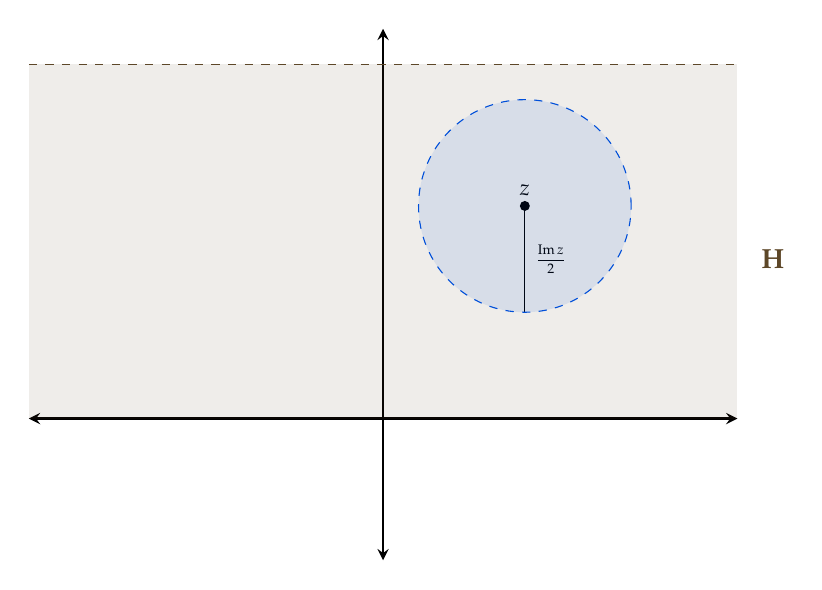
\begin{tikzpicture}[scale=0.9]
    \draw[<->,thick] (-5,0)--(5,0);
	\draw[<->,thick] (0,-2)--(0,5.5);
    \node[] at (5.5,2.25) {\color{dirt}$\mathbf{H}$};
	\draw[dashed,dirt] (-5,5)--(5,5);
    \fill[dirt,fill opacity=1/10](-5,0) -- (-5,5) -- (5,5) -- (5,0);
    
    \fill (2,3) circle (2pt) node[above]{\footnotesize$z$};
    \draw[](2,3)--(2,1.5) node[midway,right]{\tiny$\dfrac{\Im z}{2}$};
    \filldraw[newblue,fill opacity=1/10,dashed](2,3) circle (1.5);
  \end{tikzpicture}\]
\lecmargin{8}
Let $w \in D_\epsilon(z)$, then \[\abs{w - z} < \epsilon = \frac{\Im z}{2}\]
The end of Discussion \ref{cmplxnorm} tells us
\begin{align*}
\frac{\Im z}{2} > \abs{w - z} &\geq \abs{\Im(w - z)}\\[0.5em]
&= \abs{\Im w - \Im z}
\end{align*}
The later is simply the absolute value of a real number, which gives
\[-\frac{\Im z}{2} < \Im w - \Im z < \frac{\Im z}{2}\]
Adding $\Im z$ throughout the inequality, we get from the inequality on the left hand side
\[\Im w > \frac{\Im z}{2} > 0.\]
Therefore $w \in \mathbf{H}$, and hence $D_\epsilon(z) \subseteq \mathbf{H}$. Thus $\mathbf{H}^\circ = \mathbf{H}$.\\[1em]
The points exterior to $\mathbf{H}$ are points $z$ such that $\Im z < 0$. That is, the exterior of the upper half-plane is the (open) lower half-plane. The boundary of $\mathbf{H}$ consists of precisely points $z$ whose $\Im z = 0$. That is, $\partial \mathbf{H} = \rr$.\\[0.5em]
The closure of $\mathbf{H}$ is $\overline{\mathbf{H}} = \setp{z\in \cc}{\Im z\geq 0}$. While $\mathbf{H} \cup \set{0}$ is neither open nor closed.
\end{itemize}
\end{example}

\medskip

\begin{definition}[Bounded Sets]
A set $S \subseteq \cc$ is \cdef{bounded} if $S \subseteq D_M(0)$ for some $M>0$. That is, there exists an $M>0$ such that $\abs{z} \leq M$ for every $z \in S$.
\end{definition}

\medskip

\begin{definition}[Connected Sets]
A set $S \subseteq \cc$ is said to be \cdef{connected} if each pair of points $z_1$ and $z_2$ in $S$ can be joined by a \emph{polygonal line}, consisting of a finite number of line segments joined end to end, that lies entirely in $S$. Otherwise, we say it is \cdef{disconnected}.
\[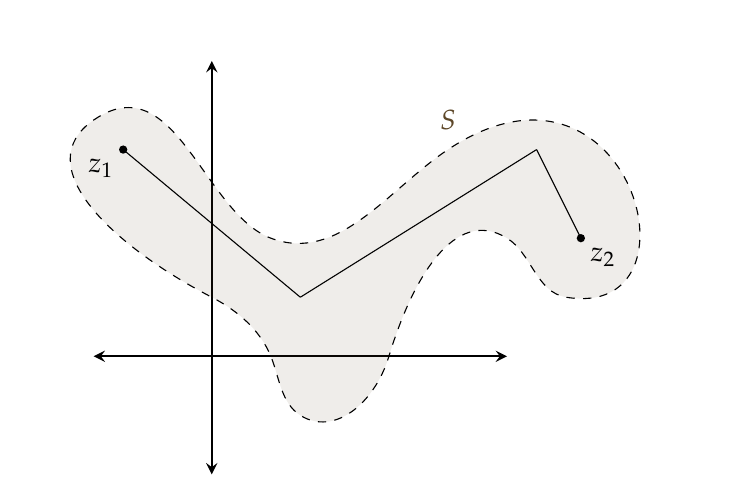
\begin{tikzpicture}[scale=0.75]
    \draw[<->,thick] (-2,0)--(5,0);
	\draw[<->,thick] (0,-2)--(0,5);
    \node[] at (4,4) {\color{dirt}$S$};
    \path[draw,use Hobby shortcut,closed=true,fill=dirt,fill opacity=1/10,dashed]
%(-1,0) .. (3,0) .. (3,4) .. (1.5,2) .. (-1,0);
(-2,4) .. (1,2) .. (4,3.5) .. (6,1) .. (5,2) .. (3,0) .. (1.5,-1) .. (1,0) .. (0,1) .. (-2,4);
    \draw[](-1.5,3.5)--(1.5,1);
    \draw[](1.5,1)--(5.5,3.5);
    \draw[](5.5,3.5)--(6.25,2);
    \fill (-1.5,3.5) circle (2pt) node[below left]{$z_1$};
    \fill (6.25,2) circle (2pt) node[below right]{$z_2$};
%    \fill (1.5,1) circle (2pt);
%    \fill (5.5,3.5) circle (2pt);
\end{tikzpicture}\]
\end{definition}

\medskip

\begin{definition}[Domain]
$S \subseteq \cc$ is called a \cdef{domain} if it's a non-empty open and connected set.\\[0.5em]
A \cdef{region} is a domain together with some or all of its boundary points.
\end{definition}

\medskip

\begin{remark}
Domains and regions are sets we will find most suitable for stating elegant results about certain functions in a complex variable.
\end{remark}

\medskip

\begin{example}
$\mathbf{H}$ is a domain since it's non-empty, open and any two points in $\mathbf{H}$ can be connected by a straight line. It's an unbounded set. An example of a region is $\mathbf{H} \cup \set{0}$.
\end{example}
\newpage

\section{Part II. Holomorphic Functions}
\subsection{Complex Functions}

%\begin{mdframed}[backgroundcolor=paleyellow,linewidth=1pt]
%\begin{center}
%{\sc\Large Part II. Holomorphic Functions}
%\end{center}
%\end{mdframed}
%
%\begin{mdframed}
%\begin{center}
%{\Large Complex Functions}
%\end{center}
%\end{mdframed}

\begin{definition}
A \emph{function} $f:G \to \cc$ is a rule that assigns to each $z\in G$ a unique number $f(z) \in \cc$.\\[0.5em]
The set $G$ is called the \emph{domain (of definition)}. If $S \subseteq G$, then
\[f(S) \coloneqq \setp{f(z)}{z\in S}\]
is called the \emph{image of $S$ under $f$}.\\[0.5em]
The set $f(G)$ is called the \emph{image (or range) of $f$}. Points in $f(G)$ are called \emph{values of $f$}.\\[1em]
Given a function $f$, we define its conjugate $\bar{f}$ by the rule $\bar{f}(z) \coloneqq \overline{f(z)}$.
\end{definition}

\medskip

\begin{discussion}
\lecmargin{9}
If $f:G \to \cc$ is a function, then the value $f(x+iy) = u + iv$ depends on a pair $(x,y) \in \rr^2$. Collecting all values, we decompose $f$ into its \cdef{real} and \cdef{imaginary\ parts}
\[f(z) = f(x+iy) = u(x,y) + i\,v(x,y);\quad \Re f = u \ \text{ and } \ \Im f = v,\] where $u,v: \rr^2 \to \rr$ are real-valued functions in two real variables.\\[1em]
In practice, as the examples below tell us, this means replace your $z = x + iy$ and do the required operations to the output $f(x + iy)$. The resulting complex number will be, as a complex number, of the form $u + iv$. The real part is $u$, which you will obtain in terms of $x$ and $y$, and the imaginary part is $v$, which you will also obtain in terms of $x$ and $y$. 
\end{discussion}

\medskip

\begin{example}[Some Complex Functions]\hfill
\begin{itemize}
\item[(1)] $f(z) = z^2 = (x+iy)^2 = (x^2 - y^2) + i(2xy)$. So, \[u(x,y) = x^2 - y^2 \quad \text{and} \quad v(x,y) = 2xy.\]
\item[(2)] $f(z) = \overline{z} = x-iy$. So, \[u(x,y) = x \quad \text{and} \quad v(x,y) = -y.\]
\item[(3)] (in-class) $f(z) = z\overline{z} = \abs{z}^2 = x^2+y^2$. So, \[u(x,y) = x^2 + y^2 \quad \text{and} \quad v(x,y) = 0.\]
Such a function is \emph{real-valued}.
\item[(4)] \emph{Polynomials of degree $n$} are functions of the form \[p(z) = a_0 + a_1z + \cdots a_nz^n,\] where $a_i \in \cc$ and $a_n \neq 0$.\\[1em]
A polynomial of degree $0$ is simply a non-zero complex number, sometimes also referred to as a \emph{constant polynomial}.
\item[(5)] \emph{Rational functions (or polynomials)} are functions of the form
\[\dfrac{p(z)}{q(z)}\]
where $p(z)$ and $q(z)$ are polynomials. The domain of definition is wherever $q(z) \neq 0$. For example,
\[f:\cc^* \to \cc,\ z \mapsto \frac{1}{z}\]
\item[(6)] If we express $z$ in its polar form, then a function $f$, when we restrict its domain of definition within $\cc^*$, can be written as
\[f(z) = f(re^{i\theta}) = u(r,\theta) + i\,v(r,\theta)\]
For example,
\[f:\cc^* \to \cc,\ z = re^{i\theta} \mapsto \frac{1}{z} = \frac{1}{r}e^{-i\theta} = \frac{\cos\theta}{r} - i\,\frac{\sin\theta}{r}.\]
Here $u(r,\theta) = \dfrac{\cos\theta}{r}$ and $v(r,\theta) = -\dfrac{\sin\theta}{r}$.
\item[(7)] (in-class) Let's consider the function $f(z) = \overline{z}^2$, in polar form we have
\begin{align*}
f(re^{i\theta}) &= (\overline{re^{i\theta}})^2\\[0.5em]
&= (re^{-i\theta})^2,\quad \text{by Proposition \ref{propeuler} (4)}\\[0.5em]
&= r^2e^{-i2\theta},\quad \text{by Proposition \ref{propeuler} (3)}\\[0.5em]
&= r^2(\cos(-2\theta) + i\sin(-2\theta))\\[0.5em]
&= r^2\cos(2\theta) - i\sin(2\theta))
\end{align*}
Therefore, here $u(r,\theta) = r^2\cos(2\theta)$ and $v(r,\theta) = -r^2\sin(2\theta)$.
\item[(8)] Consider $f(z) = z^{1/n}$, where $n$ is a non-zero integer. For no $n \neq 1$ is this a function! We have seen previously that $z^{1/n}$ has $n$-distinct values. Such a "function" is called multi-valued.\\[1em]
We can make this into a (single-valued) function by assigning a single value of $z^{1/n}$ to each $z$; taking the \emph{principal $n^{\text{th}}$ root of $z$}, for instance. More on such functions soon. 
\end{itemize}
\end{example}

\bigskip

\subsection{Limits of Functions}
%\begin{mdframed}
%\begin{center}
%{\Large Limits of Functions}
%\end{center}
%\end{mdframed}

\begin{definition}[Limit of a Function]\label{limdef}
Consider a function $f:G \to \cc$, and an accumulation point $z_0$ of $G$.\\[0.5em]
We say that \cdef{limit} of $f$, as $z$ approaches $z_0$, is $w_0 \in \cc$ if \emph{for all $\epsilon > 0$ there exists a $\delta > 0$ such that
\[\text{if }\ 0 < \abs{z - z_0} < \delta,\quad \text{then }\ \abs{f(z) - w_0}<\epsilon\]}\\
Equivalently, if $z \in D_{\delta}(z_0)\setminus \set{z_0}$, then $f(z) \in D_\epsilon(w_0)$.
\[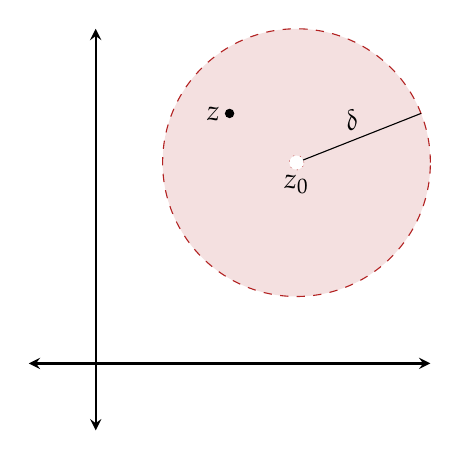
\begin{tikzpicture}[scale=0.85]
    \draw[<->,thick] (-1,0)--(5,0);
	\draw[<->,thick] (0,-1)--(0,5);
	\filldraw[firebrick,fill opacity=1/7,dashed](3,3) circle (2);
    \draw[firebrick,dotted](3,3) circle (3pt);    
    \draw[](3,3)--(4.86,3.735) node[sloped,midway,above]{$\delta$};
    \fill[white] (3,3) circle (3pt) node[below,yshift=-1pt]{\color{black}$z_0$};
    \fill (2,3.735) circle (2pt) node[left]{$z$};
  \end{tikzpicture}
  \qquad\qquad\qquad
  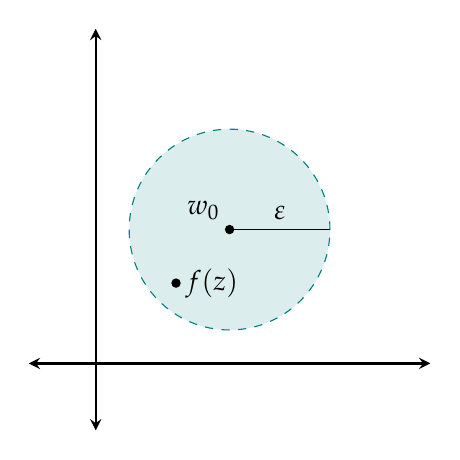
\begin{tikzpicture}[scale=0.85]
    \draw[<->,thick] (-1,0)--(5,0);
	\draw[<->,thick] (0,-1)--(0,5);
	\filldraw[teal,fill opacity=1/7,dashed](2,2) circle (1.5);
    \draw[](2,2)--(3.5,2) node[sloped,midway,above]{$\epsilon$};
    \fill (2,2) circle (2pt) node[above left]{$w_0$};
    \fill (1.2,1.2) circle (2pt) node[right]{$f(z)$};
  \end{tikzpicture}\]
In this case we write $\lim_{z \to z_0}f(z) = w_0$ or $f(z) \to w_0,\ \text{as } z \to z_0$.\\
\\
Intuitively, the limit of $f$ at $z_0$ is $w_0$ if \[\text{"$f$ is arbitrarily close to $w_0$ eventually, that is sufficiently, near $z_0$".}\] How close? Within an error of $\epsilon$. How near, eventually? Within a distance of $\delta$.
\end{definition}

\medskip

\begin{example}
\lecmargin{10}
Let's show that $\lim_{z \to i} z^2 = -1$ using the definition.
\end{example}
\begin{proof}
Let $\epsilon > 0$ be arbitrary. Note that $\abs{z^2 - (-1)} = \abs{z - i}\abs{z + i}$. We make an initial estimate, suppose $0 < \abs{z - i} < 1$, then
\begin{align*}
\abs{z + i} &= \abs{z - i + 2i}\\[0.5em]
&\leq \abs{z - i} + \abs{2i}\\[0.5em]
&< 1 + 2\\[0.5em]
&= 3
\end{align*}
Now, if we choose $\delta = \min\set{\dfrac{\epsilon}{3},1}$, then if $0 < \abs{z - i} < \delta$ we get
\[0 < \abs{z - i} < 1\ \text{and}\ \frac{\epsilon}{3}\]
So,
\begin{align*}
\abs{z^2 - (-1)} &= \abs{z - i}\abs{z + i}\\[0.5em]
&< 3\abs{z - i},\quad \text{since $\abs{z - i} < 1$}\\[0.5em]
&< 3\cdot\frac{\epsilon}{3},\quad \text{since $\abs{z - i} < \frac{\epsilon}{3}$}\\[0.5em]
&= \epsilon
\end{align*}
Therefore $\lim_{z \to i} z^2 = -1$.
\end{proof}

\medskip

\begin{theorem}\label{limunique}
If $f$ has a limit at $z_0$, then it is unique.
\end{theorem}
\begin{proof}
Assume
\[\lim_{z \to z_0}f(z) = \alpha \quad \text{and} \quad \lim_{z \to z_0}f(z) = \beta\]
Consider an arbitrary $\epsilon > 0$, then we can find a $\delta_1 > 0$ such that
\[\text{if }\ 0 < \abs{z - z_0} < \delta,\quad \text{then }\ \abs{f(z) - \alpha}<\frac{\epsilon}{2}\]
and $\delta_2 > 0$ such that
\[\text{if }\ 0 < \abs{z - z_0} < \delta,\quad \text{then }\ \abs{f(z) - \beta}<\frac{\epsilon}{2}\]
Define $\delta \coloneqq \min\set{\delta_1,\delta_2} \leq \delta_1,\,\delta_2$, then if $0< \abs{z - z_0} < \delta$ we have
\begin{align*}
\abs{\alpha - \beta} &= \abs{f(z) - f(z) + \alpha - \beta}\\[0.5em]
&\leq \abs{\alpha - f(z)} + \abs{f(z) - \beta}\\[0.5em]
&= \abs{f(z) - \alpha} + \abs{f(z) - \beta}\\[0.5em]
&< \frac{\epsilon}{2} + \frac{\epsilon}{2}\\[0.5em]
&= \epsilon
\end{align*}
We have proven that $\abs{\alpha - \beta} < \epsilon$ for any $\epsilon > 0$. Now, suppose $\alpha \neq \beta$, then for $\epsilon = \abs{\alpha - \beta} > 0$ we get $\abs{\alpha - \beta} < \abs{\alpha - \beta}$, which is preposterous. Hence $\alpha = \beta$, and thus the limit is unique.
\end{proof}

\medskip

\begin{remark}
The reason we require that $z_0$ be an accumulation point of the domain of $f$ is just that we need to be sure that there are points $z$ of the domain that are arbitrarily close to $z_0$. That is, there are indeed points satisfying $0< \abs{z-z_0} < \delta$.\\[0.5em]
Our definition (i.e., the part that says $0 < \abs{z - z_0}$) does not require $z_0$ to be in the domain of $f$, and if $z_0$ is in the domain of $f$, the definition explicitly ignores the value of $f(z_0)$.
\end{remark}

\medskip

Uniqueness of limits can be used to show that a limit does not exist.
\begin{example}\label{limnotex}
The function $f(z) = \dfrac{\overline{z}}{z}$ has no limit at $0$.
\end{example}
\begin{proof}[Discussion of Example \ref{limnotex}]
Let $z = x + iy$, then
\[f(z) = \frac{x - iy}{x + iy}\]
Along the real axis, $\Im z = 0$, and so $z = x$, giving us $f(z) = \dfrac{x}{x} = 1$.\\[0.5em]
Along the imaginary axis, $\Re z = 0$, and so $z = y$, giving us $f(z) = \dfrac{-y}{y} = -1$.\\[0.5em]
Taking the limit along these axes gives us different values of the limit, $1$ and $-1$. Hence, by the uniqueness of limits, the limit doesn't exist.
\end{proof}

\bigskip

\subsection{Theorems on Limits}
%\begin{mdframed}
%\begin{center}
%{\Large Theorems on Limits}
%\end{center}
%\end{mdframed}

\begin{theorem}[Limit in terms of Real and Imaginary parts of a Function]\label{cmplxlimripart}
Suppose that
\[f(z) = f(x + iy) = u(x,y) + i\,v(x,y)\]
Then 
\[\lim_{x + iy \to x_0 + iy_0}f(x + iy) = u_0 + iv_0\]
if and only if
\[\lim_{(x,y) \to (x_0,y_0)}u(x,y) = u_0 \quad \text{and} \quad \lim_{(x,y) \to (x_0,y_0)}v(x,y) = v_0\]
\end{theorem}
\begin{proof}
$(\Rightarrow)$ Consider an arbitrary $\epsilon > 0$, then there exists a $\delta > 0$ such that if
\[0 < \abs{(x+iy) - (x_0 + iy_0)} < \delta\]
\[\text{then }\ \abs{f(x+iy) - (u_0 + iv_0)} = \abs{(u(x,y) + i\,v(x,y)) - (u_0 + iv_0)} < \epsilon\]
We first note that, by definition
\begin{align*}
\norm{(x,y) - (x_0,y_0)} &= \abs{(x+iy) - (x_0 + iy_0)}
\end{align*}
and the end of Discussion \ref{cmplxnorm} tells us that
\begin{align*}
\abs{u(x,y) - u_0} &\leq \abs{(u(x,y) + i\,v(x,y)) - (u_0 + iv_0)} < \epsilon\\[0.5em]
\abs{v(x,y) - v_0} &\leq \abs{(u(x,y) + i\,v(x,y)) - (u_0 + iv_0)} < \epsilon
\end{align*}
That is, we have that
\[\text{if }\ 0 < \norm{(x,y) - (x_0,y_0)} < \delta,\quad \text{then }\ \abs{u(x,y) - u_0} < \epsilon\ \ \text{and}\ \ \abs{v(x,y) - v_0} < \epsilon\]
Therefore,
\[\lim_{(x,y) \to (x_0,y_0)}u(x,y) = u_0 \quad \text{and} \quad \lim_{(x,y) \to (x_0,y_0)}v(x,y) = v_0\]\\[1em]
$(\Leftarrow)$ Consider an arbitrary $\epsilon > 0$, then there exists a $\delta_1 > 0$ such that
\[\text{if }\ 0 < \norm{(x,y) - (x_0,y_0)} < \delta_1,\quad \text{then }\ \abs{u(x,y) - u_0} < \frac{\epsilon}{2}\]
and there exists a $\delta_2 > 0$ such that
\[\text{if }\ 0 < \norm{(x,y) - (x_0,y_0)} < \delta_2,\quad \text{then }\ \abs{v(x,y) - v_0} < \frac{\epsilon}{2}\]
Define $\delta \coloneqq \min\set{\delta_1,\delta_2} \leq \delta_1,\,\delta_2$. Now, if
\[0 < \abs{(x+iy) - (x_0 + iy_0)} = \norm{(x,y) - (x_0,y_0)} < \delta\]
then
\begin{align*}
\abs{f(x+iy) - (u_0 + iv_0)} &= \abs{(u(x,y) + i\,v(x,y)) - (u_0 + iv_0)}\\[0.5em]
&= \abs{(u(x,y) - u_0) + i(v(x,y)- v_0)}\\[0.5em]
&\leq \abs{(u(x,y) - u_0)} + \abs{i(v(x,y)- v_0)},\ \text{by triangle identity}\\[0.5em]
&= \abs{(u(x,y) - u_0)} + \abs{i}\abs{(v(x,y)- v_0)}\\[0.5em]
&= \abs{(u(x,y) - u_0)} + \abs{(v(x,y)- v_0)}\\[0.5em]
&< \frac{\epsilon}{2} + \frac{\epsilon}{2}\\[0.5em]
&= \epsilon
\end{align*}
Therefore,
\[\lim_{x + iy \to x_0 + iy_0}f(x + iy) = u_0 + iv_0\]
\end{proof}

\medskip

\begin{theorem}[Limit Laws]\label{limlaw}
Suppose
\[\lim_{z \to z_0} f(z) = \alpha \quad \text{and} \quad \lim_{z \to z_0} g(z) = \beta\]
Then
\begin{itemize}
\item[(1)] $\lim_{z \to z_0} (f(z) + g(z)) = \alpha + \beta$
\item[(2)] $\lim_{z \to z_0} (f(z)\,g(z)) = \alpha\beta$
\item[(3)] $\lim_{z \to z_0} \dfrac{f(z)}{g(z)} = \dfrac{\alpha}{\beta}$, provided $\beta \neq 0$.
\end{itemize}
\end{theorem}
\begin{proof}
The proof follows from Theorem \ref{cmplxlimripart} and limit laws from Calculus.
\end{proof}

\medskip

\begin{example}\label{polycts}
Let $p(z)$ be a polynomial, then
\[\lim_{z \to z_0}p(z) = p(z_0)\]
Write $p(z) = a_0 + a_1z + \cdots + a_nz^n$, then by Theorem \ref{limlaw} we have
\begin{align*}
\lim_{z \to z_0}p(z) &= \lim_{z \to z_0}(a_0 + a_1z + \cdots + a_nz^n)\\[0.5em]
&= \lim_{z \to z_0} a_0 + \lim_{z \to z_0} a_1z + \cdots + \lim_{z \to z_0} a_nz^n,\ \text{by Theorem \ref{limlaw} (1)}\\[0.5em]
&= \lim_{z \to z_0} a_0 + \lim_{z \to z_0} a_1 \cdot \lim_{z \to z_0} z + \cdots + \lim_{z \to z_0} a_n \cdot \lim_{z \to z_0} z^n,\ \text{by Theorem \ref{limlaw} (2)}\\[0.5em]
&= a_0 + a_1z_0 + \cdots + a_nz_0^n,\ \text{by Theorem \ref{limlaw} (2) and }\lim_{z \to z_0} z = z_0\\[0.5em]
&= p(z_0)
\end{align*}\\[-2em]
\qed
\end{example}

\bigskip

\begin{definition}[Extended Complex Plane or the Riemann Sphere]
\lecmargin{11}
The \cdef{Extended\ Complex\ Plane} is the set $\cc$ together with a symbol $\infty$ called the \emph{point at infinity}, denoted $\widehat{\cc}$ or $\cc_\infty$.\\[0.5em]
There is a bijection between the extended complex plane and the unit sphere given by the \emph{stereographic projection}, and therefore the extended complex plane is also called the \cdef{Riemann\ Sphere}.\\
\[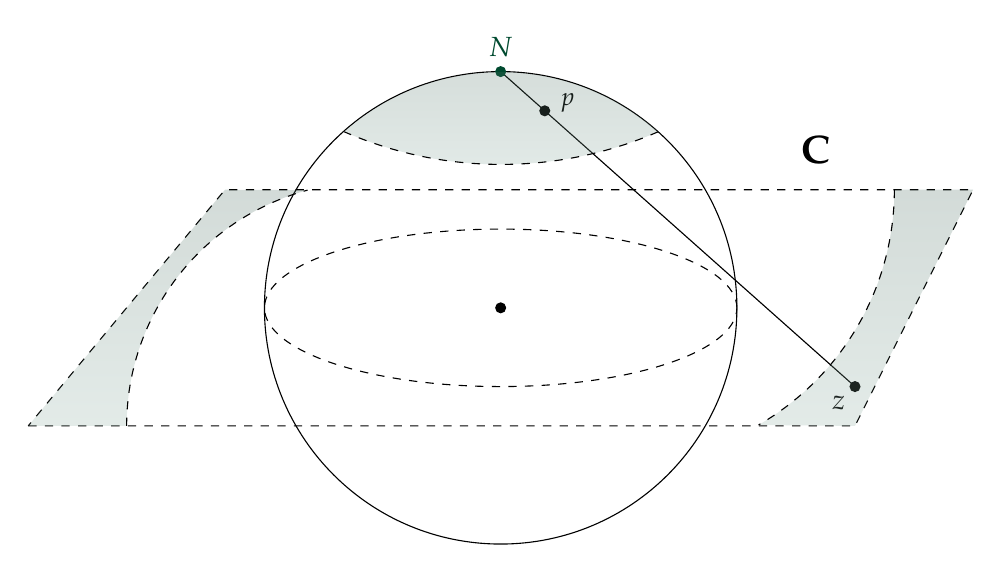
\begin{tikzpicture}
  \draw[dashed] (-6,-1.5) -- (4.5, -1.5) -- (6, 1.5) -- (-3.5,1.5) -- (-6,-1.5);
  \draw (0,0) circle (3);
  \draw[dashed] (0,0) ellipse (3 and 1);
  \draw[] (0,3) -- (4.5, -1);
  \fill[forest] (0,3) circle (2pt) node[above,yshift=2pt]{{\color{forest}$N$}};
  \fill (0, 0) circle (2pt);
  \fill (4.5, -1) circle (2pt) node[below left]{$z$};
  \fill (0.56, 2.502) circle (2pt) node[right,yshift=3pt,xshift=2pt]{\small$p$};
  \shade[fill=forest,fill opacity=1/8] (5,1.5) arc (0:-60:3.45) -- (4.5,-1.5) -- (6,1.5) -- (5,1.5);
  \draw[dashed] (5,1.5) arc (0:-60:3.45);
  \shade[fill=forest,fill opacity=1/8] (-4.75,-1.5) arc (0:-75:-3.1) -- (-3.5,1.5) -- (-6,-1.5) -- (-4.75,-1.5);
  \draw[dashed] (-4.75,-1.5) arc (0:-75:-3.1);
  \shade[fill=forest,fill opacity=1/8] (2,2.236) arc (113.5:66.5:-5) arc (-48.35:-131.8:-3);
  \draw[dashed] (2,2.236) arc (113.5:66.5:-5);
  \node[] at (4,2) {\Large$\cc$};
\end{tikzpicture}\]\\
The point $N$ (the north pole) corresponds to $\infty$, and any point $p$ on the sphere corresponds uniquely to a point $z \in \cc$ which is the unique point of intersection of the complex plane with the line passing through $N$ and $p$.
\end{definition}

\medskip

\begin{definition}[Neighbourhood of Infinity]
Let $\epsilon > 0$, the set
\[\setp{z\in \cc}{\abs{z} > \frac{1}{\epsilon}}\]
is called a \emph{neighbourhood of $\infty$}. Geometrically, a neighbourhood at infinity is the exterior of a circle centered at the origin, which corresponds to a neighbourhood of $N$ on the unit sphere.
\end{definition}

\medskip

\begin{discussion}
We can now easily give meaning to limits
\[\lim_{z \to z_0}f(z) = w_0\]
where $z_0$ and $w_0$ are allowed to be $\infty$. We replace the appropriate neighbourhood in  Definition \ref{limdef} with neighbourhoods of $\infty$.
\end{discussion}

\medskip

\begin{theorem}[Limits involving Infinity]\hfill
\begin{itemize}
\item[(1)] $\displaystyle\lim_{z \to z_0} \dfrac{1}{f(z)} = 0$ if and only if $\displaystyle\lim_{z \to z_0}f(z) = \infty$.
\item[(2)] $\displaystyle\lim_{z \to \infty}f(z) = \lim_{z \to 0} f\left(\dfrac{1}{z}\right)$, provided the limit exist.
\end{itemize}
\emph{Combining (1) and (2), we get \[\displaystyle\lim_{z \to 0} \dfrac{1}{f\left(\frac{1}{z}\right)} = 0\quad \text{if and only if} \quad \displaystyle\lim_{z \to \infty}f(z) = \infty.\]}
Bottom line, we can simplify limits involving $\infty$ to limits involving $0$.
\end{theorem}
\begin{proof}
The proofs are based on the simple observation that
\[\frac{1}{a} < b \quad \text{if and only if} \quad \frac{1}{b} < a\]
for non-zero real numbers $a$ and $b$.
\begin{itemize}
\item[(1)] Now $\displaystyle\lim_{z \to z_0} \dfrac{1}{f(z)} = 0$ if and only if for every $\epsilon > 0$ there exists $\delta > 0$ such that 
\[\text{if }\ 0 < \abs{z - z_0} < \delta,\quad \text{then }\ \frac{1}{\abs{f(z)}} = \abs{\frac{1}{f(z)} - 0}< \epsilon\]
if and only if for every $\epsilon > 0$ there exists $\delta > 0$ such that 
\[\text{if }\ 0 < \abs{z - z_0} < \delta,\quad \text{then }\ \abs{f(z)}>\frac{1}{\epsilon}\]
if and only if
$\displaystyle\lim_{z \to z_0}f(z) = \infty$.
\item[(2)] $\displaystyle\lim_{z \to \infty}f(z) = \alpha$ if and only if for every $\epsilon > 0$ there exists $\delta > 0$ such that 
\[\text{if }\ \abs{z} > \frac{1}{\delta},\quad \text{then }\ \abs{f(z) - \alpha}< \epsilon\]
if and only if for every $\epsilon > 0$ there exists $\delta > 0$ such that 
\[\text{if }\ 0 < \abs{\frac{1}{z}} < \delta,\quad \text{then }\ \abs{f(z) - \alpha} < \epsilon\]
if and only if, by replacing $z$ with $1/z$, $\displaystyle\lim_{z \to 0}\,f\left(\dfrac{1}{z}\right) = \alpha$.
\end{itemize}
\end{proof}

\medskip

\begin{example}
We want to show $\displaystyle \lim_{z \to \infty} \frac{2z^4 + 1}{z^3 + 1} = \infty$. This is equivalent to showing
\[\lim_{z \to 0} \frac{1}{f(1/z)} = \lim_{z \to 0} \frac{(1/z)^3 + 1}{2(1/z)^4 + 1} = 0,\quad \text{for }f(z) = \frac{2z^4 + 1}{z^3 + 1}\]
Note that,
\begin{align*}
\lim_{z \to 0} \frac{(1/z)^3 + 1}{2(1/z)^4 + 1}&= \lim_{z \to 0} \frac{\frac{1 + z^3}{z^3}}{\frac{2 + z^4}{z^4}}\\[0.5em]
&= \lim_{z \to 0}\ z\cdot\frac{1 + z^3}{2 + z^4}\\[0.5em]
&= 0\cdot\frac{1}{2}\\[0.5em]
&= 0
\end{align*}
Therefore $\displaystyle \lim_{z \to \infty} \frac{2z^4 + 1}{z^3 + 1} = \infty$.
\end{example}

\medskip

\begin{example}[in-class]
Show $\displaystyle \lim_{z \to \infty} \frac{2 + z^5}{z^2 + 3} = \infty$.
\end{example}
\begin{proof}[Answer]
This is equivalent to showing
\[\lim_{z \to 0} \frac{1}{f(1/z)} = \lim_{z \to 0} \frac{(1/z)^2 + 3}{2 + (1/z)^5} = 0,\quad \text{for }f(z) = \frac{2 + z^5}{z^2 + 3}\]
Note that,
\begin{align*}
\lim_{z \to 0} \frac{(1/z)^2 + 3}{2 + (1/z)^5} &= \lim_{z \to 0} \frac{\frac{1 + 3z^2}{z^2}}{\frac{2z^5 + 1}{z^5}}\\[0.5em]
&= \lim_{z \to 0}\ z^3\cdot\frac{1 + 3z^2}{2z^5 + 1}\\[0.5em]
&= 0^3\cdot\frac{1}{1}\\[0.5em]
&= 0
\end{align*}
Therefore $\displaystyle \lim_{z \to \infty} \frac{2 + z^5}{z^2 + 3} = \infty$.
\end{proof}

\bigskip

\subsection{Continuous Functions}
%\begin{mdframed}
%\begin{center}
%{\Large Continuous Functions}
%\end{center}
%\end{mdframed}

\begin{definition}[Continuous Functions]
A function $f: G \to \cc$ is \emph{continuous at $z_0 \in G$} if either $z_0$ is an isolated point or 
\[\lim_{z \to z_0}\,f(z) = f(z_0) = f\left(\lim_{z\to z_0}\,z\right)\]
That is, for all $\epsilon > 0$, there exists a $\delta > 0$ such that
\[\text{if }\ 0 < \abs{z - z_0} < \delta,\quad \text{then }\ \abs{f(z) - f(z_0)}<\epsilon.\]
A function is \cdef{continuous} if it is continuous at every point in its domain.\\
\\
By the limit laws (Theorem \ref{limlaw}), sum, product and quotient of continuous functions are continuous (whenever and wherever defined).
\end{definition}

\medskip

\begin{theorem}[Composition of Continuous Functions]\label{composcont}
Suppose we have two functions $f:G_1 \to \cc$ and $g: G_2 \to \cc$ such that $f(G_1) \subseteq G_2$. If $f$ is continuous at $z_0$ and $g$ is continuous at $f(z_0)$, then $g\circ f$ is continuous at $z_0$. That is,
\[\lim_{z \to z_0}g(f(z)) = g(f(z_0)) = g\left(\lim_{z\to z_0}f(z)\right) = g\left(f\left(\lim_{z\to z_0}\,z\right)\right)\]
Therefore, if $f$ and $g$ are continuous, so is $g\circ f$.
\end{theorem}
\begin{proof}
By continuity of $g$ at $f(z_0)$, for an arbitrary $\epsilon > 0$, there exists a $\delta_1 > 0$ such that
\[\text{if }\ 0 < \abs{w - f(z_0)} < \delta_1,\quad \text{then }\ \abs{g(w) - g(f(z_0))}<\epsilon.\]
Now, by continuity of $f$ at $z_0$, for $\delta_1 > 0$, there exists a $\delta > 0$ such that
\[\text{if }\ 0 < \abs{z - z_0} < \delta,\quad \text{then }\ \abs{f(z) - f(z_0)}<\delta_1.\]
With these two statements, we have that 
\[\text{if }\ 0 < \abs{z - z_0} < \delta,\quad \text{then }\ \abs{g(f(z)) - g(f(z_0))}<\epsilon.\]
Therefore $g\circ f$ is continuous at $z_0$.
\end{proof}

\medskip

\begin{theorem}
\lecmargin{12}
Suppose $f: G \to \cc$ is continuous at $z_0$ and $f(z_0) \neq 0$, then there exists a $\delta > 0$ such that $f(z) \neq 0$ for all $z \in D_\delta(z_0)$. That is, $\abs{f(z)} > 0$ for all $z \in D_\delta(z_0)$.
\end{theorem}
\begin{proof}
Since $f$ is continuous and non-zero at $z_0$, for $\epsilon = \dfrac{\abs{f(z_0)}}{2} > 0$ there exists a $\delta > 0$ such that
\[\text{if }\ z \in D_\delta(z_0),\quad \text{then }\ \abs{f(z) - f(z_0)}< \frac{\abs{f(z_0)}}{2}.\]
For such a $z$, the reverse triangle inequality gives us
\[\abs{\abs{f(z)} - \abs{f(z_0)}} \leq \abs{f(z) - f(z_0)}< \frac{\abs{f(z_0)}}{2};\quad \text{so, }\ -\frac{\abs{f(z_0)}}{2} < \abs{f(z)} - \abs{f(z_0)} < \frac{\abs{f(z_0)}}{2}\]
since the former is the absolute value of real numbers. Therefore, adding $\abs{f(z_0)}$ to this inequality gives us
\[\abs{f(z)} > \frac{\abs{f(z_0)}}{2} > 0\]
as needed.
\end{proof}

\medskip

\begin{theorem}[Continuity in terms of Real and Imaginary parts of a Function]\label{contpart}
Suppose that 
\[f(z) = f(x + iy) = u(x,y) + i\,v(x,y).\]
Then $f$ is continuous at $z_0 = x_0 + iy_0$ if and only if $u$ and $v$ are continuous at $(x_0,y_0)$.
\end{theorem}
\begin{proof}
This is directly follows from Theorem \ref{cmplxlimripart}.
\end{proof}

\medskip

\begin{definition}[Compact Sets]
A subset of $\cc$ is said to be \cdef{compact} if it is closed and bounded.
\end{definition}

\medskip

\begin{definition}[Bounded Functions]
A function $f: G \to \cc$ is said to be a \cdef{bounded\ function} if the image $f(G)$ is bounded. Equivalently, if there exists $M > 0$ such that $\abs{f(z)} \leq M$ for every $z \in G$.
\end{definition}

\medskip

\begin{theorem}[Extreme Value Theorem]\label{evt}
Suppose $K \subseteq \cc$ is compact, and $f: K \to \cc$ is continuous. Then $f$ is bounded, that is there exists an $M > 0$ such that $\abs{f(z)} \leq M$ for all $z \in K$, and there exists a $z_0 \in K$ such that $\abs{f(z_0)} = M$.
\end{theorem}
\begin{proof}
Since $f = u + iv$ is continuous, so are $u,v:\rr^2 \to \rr$ by Theorem \ref{contpart}.  Hence, so is
\[\abs{f(z)} = \abs{f(x + iy)} = \sqrt{u(x,y)^2 + v(x,y)^2}\]
as it's obtained as a sum, product and composition of continuous functions. This result then follows from standard Calculus, since $\abs{f}$ is a real-valued function.
\end{proof}

\bigskip

\subsection{Complex-Differentiable Functions}
%\begin{mdframed}
%\begin{center}
%{\Large Complex-Differentiable Functions}
%\end{center}
%\end{mdframed}

\begin{definition}[Derivative]\label{cmplxder}
Consider a function $f:G \to \cc$, the \cdef{derivative} \emph{of $f$ at $z_0 \in G$} is the limit
\[\frac{d}{dz}(f(z_0)) = f'(z_0) \coloneqq \lim_{z \to z_0}\frac{f(z) - f(z_0)}{z - z_0}\]
If the limit exists, we say $f$ is \emph{differentiable at $z_0$}.\\[0.5em]
A function is \cdef{differentiable} if it is differentiable at every point in its domain.
\end{definition}
Letting $h = \Delta_{z_0}z = z - z_0$, the limit can also be written as
\[f'(z_0) = \lim_{h \to 0}\frac{f(z_0 + h) - f(z_0)}{h}\]

\medskip

\begin{example}
Consider $f(z) = z^2$, then
\begin{align*}
f'(z) = \lim_{h \to 0}\frac{f(z + h) - f(z)}{h} &= \lim_{h \to 0}\frac{(z + h)^2 - z^2}{h}\\[0.5em]
&= \lim_{h \to 0}\frac{2zh + h^2}{h}\\[0.5em]
&= \lim_{h \to 0}\,2z + h\\[0.5em]
&= 2z
\end{align*}
\end{example}

\medskip

\begin{example}\label{normdiffexistence}
\lecmargin{13}
Where is $f(z) = \abs{z}^2$ differentiable?\\[1em]
Consider $z \in \cc$ and an arbitrary $h \in \cc$, then we compute
\begin{align*}
f(z + h) - f(z) &= \abs{z + h}^2 - \abs{z}^2\\[0.5em]
&= (z + h)\overline{(z + h)} - z\overline{z}\\[0.5em]
&= z\overline{z} + z\overline{h} + \overline{z}h + h\overline{h} - z\overline{z}\\[0.5em]
&= z\overline{h} + \overline{z}h + h\overline{h}
\end{align*}
Then 
\[\frac{f(z + h) - f(z)}{h} = \frac{z\overline{h} + \overline{z}h + h\overline{h}}{h} = z\,\frac{\overline{h}}{h} + \overline{z} + \overline{h}\]
Along the real axis, $h = \overline{h}$, we have
\[\frac{f(z + h) - f(z)}{h} = z + \overline{z} + h;\]
therefore, as $h \to 0$, the limit is $z + \overline{z}$. Along the imaginary axis, $h = -\overline{h}$, we have
\[\frac{f(z + h) - f(z)}{h} = -z + \overline{z} - h;\]
therefore, as $h \to 0$, the limit is $-z + \overline{z}$.\\
\\
Since limits are unique, if $f'(z)$ exists, then $z + \overline{z} = -z + \overline{z}$, which gives us $z = 0$. That is, if $f'(z)$ exists, it only exists for $z = 0$. So, does $f'(0)$ exist?
\[f'(0) = \lim_{h \to 0}\frac{f(h) - f(0)}{h} = \lim_{h \to 0}\frac{h\overline{h}}{h} = \lim_{h \to 0}\overline{h} = 0\]
\end{example}

\medskip

\begin{proposition}[Differentiable Functions are Continuous]
If $f$ is differentiable at $z_0$, then $f$ is continuous at $z_0$.
\end{proposition}
\begin{proof}
Suppose $f$ is differentiable at $z_0$, then
\[\lim_{z \to z_0}f(z) - f(z_0) = \left(\lim_{z \to z_0}\frac{f(z) - f(z_0)}{z - z_0}\right)\left(\lim_{z \to z_0}\,z - z_0\right) = f'(z_0)\cdot 0 = 0\]
Therefore $\lim_{z \to z_0}f(z) = f(z_0)$, and hence $f$ is continuous at $z_0$.
\end{proof}

\medskip

\begin{theorem}[Differentiation Laws]
Suppose $f$ and $g$ are differentiable at $z$. Then,
\begin{itemize}[itemsep=1em]
\item[(1)] $(c)' = 0$, for every $c \in \cc$.
\item[(2)] $(c\cdot f)'(z) = c\cdot f'(z)$, for every $c \in \cc$.\hfill \emph{(Constant Rule)}
\item[(3)] $(z^n)' = nz^{n-1}$, for every $n \in \zz$ (assume $z \neq 0$ for $n<0$).\hfill \emph{(Power Rule)}
\item[(4)] $(f + g)'(z) = f'(z) + g'(z)$.\hfill \emph{(Sum Rule)}
\item[(5)] $(fg)'(z) = f'(z)g(z) + f(z)g'(z)$.\hfill \emph{(Product Rule)}
\item[(6)] $\left(\dfrac{f}{g}\right)'(z) = \dfrac{f'(z)g(z) - f(z)g'(z)}{g(z)^2}$, provided $g(z) \neq 0$ \hfill \emph{(Quotient Rule)}
\end{itemize}
\end{theorem}
\begin{proof}
(1) and (4) are proved directly using the limit definition, (2) can be proved directly or using (1) and (5), while (3) can be proven inductively using (5) for positive $n$ and (6) for negative $n$. 
\begin{itemize}
\item[(5)] We first compute
\begin{align*}
f(z + h)g(z + h) - f(z)g(z) &= f(z + h)g(z + h) - f(z)g(z) + f(z + h)g(z) - f(z + h)g(z)\\[0.5em]
&= f(z + h)(g(z + h) - g(z)) + g(z)(f(z + h) - f(z))
\end{align*}
So,
\begin{align*}
(fg)'(z) &= \lim_{h \to 0}\frac{f(z + h)g(z + h) - f(z)g(z)}{h}\\[0.5em]
&= \lim_{h \to 0}\frac{f(z + h)(g(z + h) - g(z))}{h} + \lim_{h \to 0}\frac{g(z)(f(z + h) - f(z))}{h}\\[0.5em]
&= \lim_{h \to 0}f(z + h)\cdot\lim_{h \to 0}\frac{g(z + h) - g(z)}{h} + g(z)\lim_{h \to 0}\frac{f(z + h) - f(z)}{h}\\[0.5em]
&= f(z)g'(z) + g(z)f'(z)
\end{align*}
\item[(6)] We first compute
\begin{align*}
\frac{1}{g(z + h)} - \frac{1}{g(z)} &= \frac{g(z) - g(z + h)}{g(z)g(z + h)}\\[0.5em]
&= -\frac{g(z+h) - g(z)}{g(z)g(z + h)}
\end{align*}
So,
\begin{align*}
\left(\dfrac{1}{g}\right)'(z) &= \lim_{h \to 0}\frac{\dfrac{1}{g(z + h)} - \dfrac{1}{g(z)}}{h}\\[0.5em]
&= \lim_{h \to 0}-\frac{g(z+h) - g(z)}{g(z)g(z + h)}\cdot\frac{1}{h}\\[0.5em]
&= -\lim_{h \to 0}\frac{g(z+h) - g(z)}{h}\cdot\lim_{h \to 0}\frac{1}{g(z)g(z + h)}\\[0.5em]
&= -\frac{g'(z)}{g(z)^2}
\end{align*}
(6) then follows from the computation above and using (5) on $\dfrac{f(z)}{g(z)} = f(z)\cdot\dfrac{1}{g(z)}$.
\end{itemize}
\vspace*{-\baselineskip}
\end{proof}

\medskip

\begin{proposition}[Chain Rule]
Suppose we have two functions $f:G_1 \to \cc$ and $g: G_2 \to \cc$ such that $f(G_1) \subseteq G_2$. If $f$ is differentiable at $z_0$ and $g$ is differentiable at $f(z_0)$, then $g\circ f$ is differentiable at $z_0$ and
\[(g\circ f)'(z_0) = g'(f(z_0))\cdot f'(z_0)\]
\end{proposition}
\begin{proof}
Let's start by defining an auxiliary function on $G_2$
\[\phi(w) = \begin{cases} \dfrac{g(w) - g(f(z_0))}{w - f(z_0)} - g'(f(z_0)) & w \neq f(z_0)\\[0.5em] 0 & w = f(z_0) \end{cases}\]
Since $g$ is differentiable at $f(z_0)$, then $\lim_{w \to f(z_0)}\phi(w) = 0 = \phi(f(z_0))$ and therefore $\phi$ is continuous at $f(z_0)$. Furthermore, since $f$ is differentiable at $z_0$, it is continuous at $z_0$. So $\lim_{z \to z_0}\phi(f(z)) = \phi(f(z_0)) = 0$ by Theorem \ref{composcont}.\\[1em]
Rewriting the above expression, we get the following expression which is valid on all of $G_2$.
\[g(w) - g(f(z_0)) = (w - f(z_0))(\phi(w) + g'(f(z_0)))\]
Now, for $w = f(z) \in f(G_1)$, we have
\begin{align*}
\frac{g(f(z)) - g(f(z_0))}{z - z_0} &= \frac{(f(z) - f(z_0))(\phi(f(z)) + g'(f(z_0)))}{z - z_0}\\[0.5em]
&= (\phi(f(z)) + g'(f(z_0)))\cdot\frac{f(z) - f(z_0)}{z - z_0}
\end{align*}
Therefore, 
\begin{align*}
(g\circ f)'(z_0) &= \lim_{z \to z_0}\frac{g(f(z)) - g(f(z_0))}{z - z_0}\\[0.5em]
&= \lim_{z \to z_0}(\phi(f(z)) + g'(f(z_0)))\cdot\lim_{z \to z_0}\frac{f(z) - f(z_0)}{z - z_0}\\[1em]
&= g'(f(z_0))\cdot f'(z_0),\ \text{since $\lim_{z \to z_0}\phi(f(z)) = 0$}
\end{align*}
\end{proof}

\bigskip

\subsection{Cauchy-Riemann Equations}
%\begin{mdframed}
%\begin{center}
%{\Large Cauchy-Riemann Equations}
%\end{center}
%\end{mdframed}
%
%When considering a real-valued function $f : \rr^2 \to \rr$ of two variables, there is no notion of the derivative of a function. For such a function, we instead only have partial derivatives $f_x(x_0,y_0)$ and $f_y(x_0,y_0)$ (and also directional derivatives) which depend on the way in which we approach a point $(x_0, y_0) \in \rr^2$. For a complex-valued function $f(z)$, we now have a new concept of the derivative $f'(z_0)$, which by definition cannot depend on the way in which we approach a point $z_0 \in \cc$. It is then natural expect a relationship between the complex derivative $f'(z_0)$ and the partial derivatives of $\Re f$ and $\Im f$, which are real-values functions. 
%
\medskip
%
\begin{theorem}[Cauchy-Riemann Equations]\label{crequations}
\lecmargin{14}
Suppose that 
\[f(z) = f(x + iy) = u(x,y) + i\,v(x,y)\]
is differentiable at $z_0 = x_0 + iy_0$. Then
\begin{itemize}
\item[(a)] the first order partial derivatives of $u$ and $v$ exist at $(x_0,y_0)$ and satisfy the \cdef{Cauchy\text{-}Riemann\ Equations}
\begin{align*}\label{creqex}
u_x(x_0,y_0) &= v_y(x_0,y_0)\\[-0.5em]
\tag{CR}\\[-0.5em]
u_y(x_0,y_0) &= -v_x(x_0,y_0)
\end{align*}
\item[(b)] $f'(z_0) = u_x(x_0,y_0) + i\,v_x(x_0,y_0) = v_y(x_0,y_0) - i\,u_y(x_0,y_0)$.
\end{itemize}
\end{theorem}
\begin{proof}
Since $f$ is differentiable at $z_0$, we have, where we let $h = s + it$
\begin{align*}
f'(z_0) &= \lim_{h\to 0}\frac{f(z_0 + h) - f(z_0)}{h}\\[0.5em]
&= \lim_{h\to 0}\frac{f((x_0 + s) + i(y_0 + t)) - f(x_0 + iy_0)}{h}\\[0.5em]
&= \lim_{h\to 0}\frac{u(x_0 + s,y_0 + t) - u(x_0,y_0)}{h} + i\cdot\lim_{h\to 0}\frac{v(x_0 + s,y_0 + t) - v(x_0,y_0)}{h}
\end{align*}
As we know by now, we must get the same result if we restrict $h$ to be on the real axis and if we restrict it to be on the imaginary axis. In the former case, $t = 0$, giving us
\begin{align*}
f'(z_0) &= \lim_{s\to 0}\frac{u(x_0 + s,y_0) - u(x_0,y_0)}{s} + i\cdot\lim_{s\to 0}\frac{v(x_0 + s,y_0) - v(x_0,y_0)}{s}\\[0.5em]
&= u_x(x_0,y_0) + i\,v_x(x_0,y_0)
\end{align*}
In the latter case, $s = 0$, giving us
\begin{align*}
f'(z_0) &= \lim_{t\to 0}\frac{u(x_0,y_0 + t) - u(x_0,y_0)}{it} + i\cdot\lim_{t\to 0}\frac{v(x_0,y_0 + t) - v(x_0,y_0)}{it}\\[0.5em]
&= \frac{1}{i}\cdot\lim_{t\to 0}\frac{u(x_0,y_0 + t) - u(x_0,y_0)}{t} + \lim_{t\to 0}\frac{v(x_0,y_0 + t) - v(x_0,y_0)}{t}\\[0.5em]
&= -i\,u_y(x_0,y_0) + v_y(x_0,y_0)
\end{align*}
Therefore
\[u_x(x_0,y_0) + i\,v_x(x_0,y_0) = f'(z_0) = v_y(x_0,y_0)-i\,u_y(x_0,y_0),\]
and hence $u_x(x_0,y_0) = v_y(x_0,y_0)$ and $u_y(x_0,y_0) = -v_x(x_0,y_0)$.
\end{proof}

\medskip

The Cauchy-Riemann equations (\ref{creqex}) are a \emph{necessary} condition for $f'$ to exist. We can use them to locate possible points where the derivative does not exist but not necessarily conclude where and if the derivative exists.
\begin{example}\label{necessarycr}\hfill
\begin{itemize}
\item[(1)] Consider $f(z) = \abs{z}^2 = x^2 + y^2$, so $u(x,y) = x^2 + y^2$ and $v(x,y) = 0$. The partial derivatives at $(x,y)$ are
\begin{align*}
u_x &= 2x & v_x &= 0\\[0.5em]
u_y &= 2y & v_y &= 0
\end{align*}
Therefore, the Cauchy-Riemann equations (\ref{creqex}) are only satisfied at $(x,y) = (0,0)$. Hence $f$ is not differentiable at any $z \neq 0$. Again, note that this does not say anything about the existence of $f'(0)$.
\item[(2)] Consider $f(z) = \overline{z} = x - iy$, so $u(x,y) = x$ and $v(x,y) = -y$. The partial derivatives at $(x,y)$ are
\begin{align*}
u_x &= 1 & v_x &= 0\\[0.5em]
u_y &= 0 & v_y &= -1
\end{align*}
Note that $u_x \neq v_y$ for all $(x,y)$ and therefore the Cauchy-Riemann equations (\ref{creqex}) are satisfied for no $(x,y)$. Hence $f$ is nowhere complex-differentiable.
\item[(3)] (in-class) Consider $f(z) = (z + i\overline{z})^2$, let's simplify $f$ to identify its real and imaginary parts $u(x,y)$ and $v(x,y)$.
\begin{align*}
f(z) &= (z + i\overline{z})^2\\[0.5em]
 &= z^2 - \overline{z}^2 + 2iz\overline{z}\\[0.5em]
 &= (z + \overline{z})(z - \overline{z}) + 2i\abs{z}^2\\[0.5em]
 &= (2\Re z)(2i \Im z) + 2i\abs{z}^2
 = 2i(\abs{z}^2 + \Re z \cdot \Im z)
\end{align*}
\begin{align*}
f(x + iy) &= 2i(x^2 + y^2 + 2xy)\\[0.5em]
&= 2i(x + y)^2
\end{align*}
Therefore $u(x,y) = 0$ and $v(x,y) = 2(x + y)^2$. The partial derivatives at $(x,y)$ are
\begin{align*}
u_x &= 0 & v_x &= 4(x + y)\\[0.5em]
u_y &= 0 & v_y &= 4(x + y)
\end{align*}
Therefore, the Cauchy-Riemann equations (\ref{creqex}) are satisfied if and only if $4(x + y) = 0$, if and only if $y = -x$. Hence $f$ is not differentiable any $z \in \cc$ such that $\Im z \neq -\Re z$.
\end{itemize}
\end{example}

\medskip

As commented, the Cauchy-Riemann equations (\ref{creqex}) are not a \emph{sufficient} condition for the existence of the derivative as the example below shows. Problem \ref{prob 7.1} gives another example.
\begin{example}\label{onlynecescr}
Consider
\[f(z) = \begin{cases}\dfrac{\overline{z}^2}{z} = \dfrac{\overline{z}^3}{\abs{z}^2} & z \neq 0\\[1em] 0 & z = 0 \end{cases}\]
Then,
\[u(x,y) = \begin{cases}\dfrac{x^3 - 3xy^2}{x^2 + y^2} & (x,y) \neq (0,0)\\[1em] 0 & (x,y) = (0,0) \end{cases} \qquad \text{and} \qquad v(x,y) = \begin{cases}\dfrac{y^3 - 3x^2y}{x^2 + y^2} & (x,y) \neq (0,0)\\[1em] 0 & (x,y) = (0,0) \end{cases}\]
We show that $u$ and $v$ satisfy the Cauchy-Riemann equations (\ref{creqex}) at $(0,0)$.
\begin{align*}
u_x(0,0) &= \lim_{s \to 0}\frac{u(s,0) - u(0,0)}{s} = \lim_{s \to 0}\frac{\dfrac{s^3}{s^2} - 0}{s} = 1\\[0.5em]
u_y(0,0) &= \lim_{t \to 0}\frac{u(0,t) - u(0,0)}{t} = \lim_{t \to 0}\frac{0 - 0}{t} = 0  \\[1em]
v_x(0,0) &= \lim_{s \to 0}\frac{v(s,0) - v(0,0)}{s} = \lim_{s \to 0}\frac{0 - 0}{s} = 0\\[0.5em]
v_y(0,0) &= \lim_{t \to 0}\frac{v(0,t) - v(0,0)}{t} = \lim_{t \to 0}\frac{\dfrac{t^3}{t^2} - 0}{t} = 1
\end{align*}
Therefore $u_x(0,0) = 1 = v_y(0,0)$ and $u_y(0,0) = 0 = -v_x(0,0)$, and hence the Cauchy-Riemann equations (\ref{creqex}) are satisfied. But $f'(0)$ does not exist, as seen in Problem \ref{prob 6.6}.
\end{example}

\medskip

Imposing certain existence and continuity conditions on the first order partial derivatives of $u$ and $v$, the Cauchy-Riemann equations (\ref{creqex}) can be upgraded to a sufficient condition for differentiability.
\begin{theorem}[Sufficient Conditions for Differentiability]\label{crsuff}
Consider a function \[f(z) = f(x + iy) = u(x,y) + i\,v(x,y)\]
and a $z_0$ in the domain of $f$, such that
\begin{itemize}
\item[(a)] the first order partial derivatives of $u$ and $v$ exist and are continuous in an open disk centered at $z_0$; and
\item[(a)] the Cauchy-Riemann equations (\ref{creqex}) are satisfied at $(x_0,y_0)$.
\end{itemize}
Then $f'(z_0)$ exists and is given by $u_x(x_0,y_0) + i\,v_x(x_0,y_0) = v_y(x_0,y_0)-i\,u_y(x_0,y_0)$.
\end{theorem}
\begin{proof}
We skip the proof. You can find a proof in \cite[Section~22, Page~66]{brown2009complex}.
\end{proof}

\medskip

\begin{example}
Let's revisit examples from Example \ref{necessarycr} and \ref{onlynecescr}.
\begin{itemize}
\item[(1)] Consider $f(z) = \abs{z}^2 = x^2 + y^2$, we noted that $u(x,y) = x^2 + y^2$ and $v(x,y) = 0$. We have seen that the only point where $f(z)$ can be differentiable is $z = 0$. The partial derivatives in a neighbourhood of $(0,0)$ are
\begin{align*}
u_x &= 2x & v_x &= 0\\[0.5em]
u_y &= 2y & v_y &= 0
\end{align*}
which clearly exist and are continuous. We have also seen that the Cauchy-Riemann equations (\ref{creqex}) are satisfied at $(0,0)$, trivially. Therefore $f'(0)$ exists and \[f'(0) = u_x(0,0) + i\,v_x(0,0) = 0.\]

\item[(2)] Consider $f(z) = (z + i\overline{z})^2$, we noted that $u(x,y) = 0$ and $v(x,y) = 2(x + y)^2$. We have seen that the only point where $f(z)$ can be differentiable are $z = x + iy \in \cc$ such that $y = \Im z = -\Re z = -x$. That is, at points of the form $(x,-x)$. The partial derivatives in a neighbourhood of $(x,-x)$ are
\begin{align*}
u_x &= 0 & v_x &= 4(x + y)\\[0.5em]
u_y &= 0 & v_y &= 4(x + y)
\end{align*}
which clearly exist and are continuous. Note the Cauchy-Riemann equations (\ref{creqex}) are satisfied at $(x,-x)$ trivially, since \[u_x(x,-x) = u_y(x,-x) = v_x(x,-x) = v_y(x,-x) = 0.\]
Therefore $f'(z)$ exists, for $z = x - ix$, and \[f'(z) = u_x(x,-x) + i\,v_x(x,-x) = 0.\]

\item[(3)] The reason Example \ref{onlynecescr} doesn't contradict Theorem \ref{crsuff} is because, $u_x$, in particular, is not continuous at $(0,0)$. Note that we have
\[u(x,y) = \begin{cases}\dfrac{x^3 - 3xy^2}{x^2 + y^2} & (x,y) \neq (0,0)\\[1em] 0 & (x,y) = (0,0) \end{cases}\]
For $(x,y) \neq (0,0)$, we compute $u_x(x,y)$ using the quotient rule, while we have already computed $u_x(0,0) = 1$ in Example \ref{onlynecescr}, giving us
\[u_x(x,y) = \begin{cases}\dfrac{x^4 + 6x^2y^2 - 3y^4}{(x^2 + y^2)^2} & (x,y) \neq (0,0)\\[1em] 1 & (x,y) = (0,0) \end{cases}\]
Suppose $u_x(x,y)$ is continuous at $(0,0)$, then we have
\[\lim_{(x,y) \to (0,0)}u_x(x,y) = \lim_{(x,y) \to (0,0)}\dfrac{x^4 + 6x^2y^2 - 3y^4}{(x^2 + y^2)^2} = u_x(0,0) = 1\]
Restricting the limit along the $y$-axis, where $x = 0$, we get
\[1 = \lim_{(0,y) \to (0,0)}\dfrac{-3y^4}{(y^2)^2} = \lim_{y \to 0}\dfrac{-3y^4}{y^4} = -3,\]
a contradiction. Hence, $u_x(x,y)$ is not continuous at $(0,0)$.
\end{itemize}
\end{example}

\medskip

\begin{example}[Complex Exponential]\label{expcmplxeg}
\lecmargin{15}
Define, for any $z = x + iy \in \cc$
\[\exp(z) = e^z \coloneqq e^xe^{iy} = e^x(\cos y + i\,\sin y)\]
the \emph{complex exponential function}. Note that $e^x$ is the usual real exponential and $e^{iy}$ is given by Euler's formula (Definition \ref{eulerform}). Here, 
\[u(x,y) = e^x\cos y \quad \text{and} \quad v(x,y) = e^x\sin y\]
We then see that
\begin{align*}
u_x &= e^x\cos y = v_y,\\[0.5em] v_x &= -e^x\sin y = -u_y;
\end{align*}
so $\exp$ satisfies the Cauchy-Riemann equations (\ref{creqex}) everywhere. Furthermore, $u_x,\,u_y,\,v_x$ and $v_y$ are everywhere defined and continuous. Hence $\exp$ is everywhere complex-differentiable, an \emph{entire} function. Furthermore $\exp(z)' = u_x + iv_x = e^x\cos y + ie^x\sin y = \exp(z)$.
\end{example}

\medskip

\begin{discussion}[Polar Cauchy-Riemann Equations]
Recall that if the domain of a function $f$ is contained in $\cc^*$ or restricted to within $\cc^*$, one can express in polar coordinates at $z = re^{i\theta}$ as
\[f(z) = f(re^{i\theta}) = u(r,\theta) + i\,v(r,\theta)\]
Then, the Cauchy-Riemann equations (\ref{creqex}) at a point $(r_0,\theta_0)$ can be expressed in polar coordinates, \cdef{Polar\ Cauchy\text{-}Riemann\ Equations} (see Problem \ref{prob 7.3})
\begin{align*}\label{pcreqex}
ru_r &= v_\theta\\[-0.5em]
\tag{Polar CR}\\[-0.5em]
u_\theta &= -rv_r
\end{align*}
and a differentiable function at $z_0 = r_0e^{i\theta_0}$ is then expressed as \[f'(z_0) = f'(r_0e^{i\theta_0}) = e^{-i\theta_0}(u_r(r_0,\theta_0) + i\,v_r(r_0,\theta_0)).\]
\end{discussion}

\medskip

\begin{example}
Consider the function
\[f(z) = f(re^{i\theta}) = \sqrt{r}\,e^{i\frac{\theta}{2}} ,\]
where $r > 0$ and $-\pi < \theta < \pi$. This is the function that outputs the principal square root of $z$. We compute $f'(z)$ at $z = re^{i\theta}$ using the polar form of Theorem \ref{crsuff}. We first note that
\[f(z) = \underbrace{\sqrt{r}\cos\left(\frac{\theta}{2}\right)}_{u(r,\theta)} + i\underbrace{\sqrt{r}\sin\left(\frac{\theta}{2}\right)}_{v(r,\theta)}\]
Now, we compute
\begin{align*}
ru_r &= r\frac{1}{2\sqrt{r}}\cos\left(\frac{\theta}{2}\right) = \frac{\sqrt{r}}{2}\cos\left(\frac{\theta}{2}\right) = v_\theta\\[0.5em]
u_\theta &= -\frac{\sqrt{r}}{2}\sin\left(\frac{\theta}{2}\right) = -r\frac{1}{2\sqrt{r}}\sin\left(\frac{\theta}{2}\right) = -rv_r
\end{align*}
Clearly the first order partial derivatives exist everywhere and the Polar Cauchy-Riemann equations (\ref{pcreqex}) are also satisfied everywhere. Hence $f'(z)$ exists and
\begin{align*}
f'(z) &= e^{-i\theta}(u_r(r,\theta) + i\,v_r(r,\theta))\\[0.5em]
&= e^{-i\theta}\left(\frac{1}{2\sqrt{r}}\cos\left(\frac{\theta}{2}\right) + i\,\frac{1}{2\sqrt{r}}\sin\left(\frac{\theta}{2}\right)\right)\\[0.5em]
&= \frac{e^{-i\theta}}{2\sqrt{r}}\left(\cos\left(\frac{\theta}{2}\right) + i\,\sin\left(\frac{\theta}{2}\right)\right)\\[0.5em]
&= \frac{1}{2\sqrt{r}}\cdot e^{-i\theta}\cdot e^{i\frac{\theta}{2}}\\[0.5em]
&= \frac{1}{2\sqrt{r}e^{i\frac{\theta}{2}}}\\[0.5em]
&= \frac{1}{2f(z)}
\end{align*}
\end{example}

\bigskip

\subsection{Holomorphic Functions}
%\begin{mdframed}
%\begin{center}
%{\Large Holomorphic Functions}
%\end{center}
%\end{mdframed}
%
\begin{definition}[Holomorphic Functions]
A function $f$ is \emph{holomorphic on an open set $U$} if $f'(z)$ exists for every $z \in U$.\\[0.5em]
We say $f$ is \emph{holomorphic at a point $z_0$} if it holomorphic on some open disk $D_\epsilon(z_0)$ for an $\epsilon > 0$. We say $f$ is \cdef{holomorphic} if it is holomorphic at every point in its domain.\\[0.5em]
A function that is holomorphic on all of $\cc$ is said to be \cdef{entire}. 
\end{definition}

\medskip

\begin{example}\hfill
\begin{itemize}
\item[(1)] $f(z) = \dfrac{1}{z}$ is holomorphic on any open set not containing $0$, in particular on $\cc^*$.
\item[(2)] $f(z) = \abs{z}^2$ is nowhere holomorphic since we have already seen that $f$ is only complex-differentiable at $z = 0$ and at no other point.
\item[(3)] Polynomials are entire.
\item[(4)] $f(z) = \overline{z}$ is nowhere holomorphic, since it's nowhere differentiable.
\end{itemize}
\end{example}

\medskip

\begin{discussion}
Let $G$ be a domain (open and connected subset of $\cc$). We know several necessary and sufficient conditions for $f = u + iv$ to be holomorphic on $G$. 
\begin{itemize}[leftmargin = 6em]
\item[(Necessary)]
\begin{itemize}
\item[(1)] $f$ is continuous on $G$.
\item[(2)] Cauchy-Riemann equations (\ref{creqex}) are satisfied on $G$.
\end{itemize}
\item[(Sufficient)]
\begin{itemize}
\item[(1)] First order partial derivatives of $u$ and $v$ exist and continuous on $G$, and the Cauchy-Riemann equations (\ref{creqex}) are satisfied on $G$.
\item[(2)] Differentiation Laws. If $f$ and $g$ are holomorphic on $G$, then so are $f + g,\, fg$ and $f/g$ (if $g \neq 0$ on $G$).
\item[(3)] Composition of holomorphic functions is holomorphic.
\end{itemize}
\end{itemize}
\end{discussion}

\medskip

\begin{theorem}[Sufficient Condition for Constantness]\label{der0const}
Suppose $G$ is a domain and $f'(z) = 0$ for all $z \in G$. Then $f(z)$ is constant on $G$.
\end{theorem}
\begin{proof}
%{\color{red}Add proof.}
Write $f(z) = f(x + iy) = u(x,y) + i\,v(x,y)$, so we have
\begin{align*}
0 = f'(z) &= u_x + iv_x = v_y - i\,u_y
\end{align*}
Therefore $u_x = u_y = 0$ and $v_x = v_y = 0$. We consider points $p,q \in G$ such that there's a line segment $L$ in $G$ connecting them. Let $\vec{w} = (a,b)$ be a unit vector parallel to $L$, then the directional derivative of $u$ along $L$ is
\[(\operatorname{grad}u)\cdot\vec{w} = au_x + bu_y = 0.\]
So, $u$ is constant along $L$. Since $G$ is a domain, any two points can be connected by a polygon line. Applying the above argument along constituent line segments, we see that $u$ has the same value along the endpoints of any polygon line. This shows that $u$ is constant on $G$, say $u(x,y) = c$. A similar argument works for $v$, giving us $v(x,y) = d$. Hence
\[f(z) = c + id,\]
that is, $f$ is constant.
\end{proof}

\medskip

Theorem \ref{der0const} has many interesting consequences.
\begin{proposition}\label{conjholconst}
Suppose $f$ and $\bar{f}$ are holomorphic on a domain $G$. Then $f$ is constant on $G$.
\end{proposition}
\begin{proof}
We write
\begin{align*}
f(z) &= f(x + iy) = u(x,y) + i\,v(x,y)\\[0.5em]
\bar{f}(z) &= \overline{f(x + iy)} = u(x,y) - i\,v(x,y)
\end{align*}
Since $f$ and $\bar{f}$ are holomorphic, they satisfy the Cauchy-Riemann equations (\ref{creqex})
\[\text{for $f$: }\ \begin{cases}u_x = v_y\\ u_y = -v_x \end{cases}\]\\[-0.5em]
\[\text{for $\bar{f}$: }\ \begin{cases}u_x = (-v)_y = -v_y\\ u_y = -(-v)_x = v_x \end{cases}\]\\
This gives us $v_y = -v_y$ and $v_x = -v_x$, and therefore $u_x = v_x = 0$. Hence $f'(z) = u_x + i\,v_x = 0$, giving us that $f$ is constant by Theorem \ref{der0const}.
\end{proof}

\medskip

\begin{corollary}\label{realholconst}
Suppose $f$ is holomorphic on a domain $G$ and always real-valued. Then $f$ is constant on $G$.
\end{corollary}
\begin{proof}
Since $f$ is always real-valued, we have $f = \bar{f}$. Therefore $\bar{f}$ is holomorphic on $G$ as well, and hence $f$ is constant by Proposition \ref{conjholconst}.
\end{proof}

\medskip

\begin{corollary}\label{absholconst}
\lecmargin{16}
Suppose $f$ is holomorphic on a domain $G$ and $\abs{f}$ is constant on it. Then $f$ is also constant on $G$.
\end{corollary}
\begin{proof}
By assumption $\abs{f(z)} = c$, for all $z \in G$, for some $c \in \cc$. This gives us
\[f(z)\overline{f(z)} = \abs{f(z)}^2 = c^2\tag{$*$}\label{eqabs}\]
Suppose $c = 0$, then $\abs{f(z)} = 0$ and therefore $f(z) = 0$. Suppose $c \neq 0$, then necessarily $f(z) \neq 0$ for every $z \in G$ by (\ref{eqabs}). Hence
\[\overline{f(z)} = \frac{c^2}{f(z)},\]
and thus $\bar{f}$ is holomorphic. Therefore both $f$ and $\bar{f}$ are holomorphic and hence $f$ is constant by Proposition \ref{conjholconst}.
\end{proof}

\medskip

\begin{example}
We apply Corollary \ref{absholconst} to $f(z) = \dfrac{\overline{z}}{z}$ to conclude that it's not holomorphic.\\
\\
We first note that, for any $z \in \cc$,
\[\abs{f(z)} = \abs{\frac{\overline{z}}{z}} = \frac{|\overline{z}|}{\abs{z}} = 1;\]
that is, $\abs{f}$ is constant. Suppose $f$ was holomorphic on $\cc$ (this argument can be specialised to any domain $G$), then $f$ would be a holomorphic function such that $\abs{f}$ is constant. Therefore, by Corollary \ref{absholconst}, $f$ is constant on $\cc$. That's a contradiction, since $f$ is non-constant, as $f(1) = 1$ and $f(i) = -1$. 
\end{example}

\medskip

\begin{example}[in-class]
Is the function $f(z) = \Re z$ holomorphic?
\end{example}
\begin{proof}[Answer]
Note that $f(z) = \Re z$ is a real-valued function, for any $z \in \cc$. Suppose $f$ was holomorphic on $\cc$ (this argument can be specialised to any domain $G$), then $f$ would be a holomorphic function such that $f$ is always real-valued. Therefore, by Corollary \ref{realholconst}, $f$ is constant on $\cc$. That's a contradiction, since $f$ is non-constant, as $f(1) = 1$ and $f(i) = 0$. 
\end{proof}

\bigskip

We now discuss a large class of holomorphic functions, which are complex  versions of functions you may have seen in your Calculus classes

\medskip

\subsection{The Exponential Function}
%\begin{mdframed}
%\begin{center}
%{\Large The Exponential Function}
%\end{center}
%\end{mdframed}
%
\begin{definition}[The Exponential Function]
The \cdef{(complex)\ exponential\, function} $e^z$ (or $\exp(z)$) is defined on all of $\cc$ as follows
\[e^z \coloneqq e^{\Re z}e^{i\Im z} = e^{\Re z}(\cos(\Im z) + i\sin(\Im z)).\]
That is, writing $z = x + iy$, we have
\[e^z = e^xe^{iy} = e^x(\cos y + i\sin y).\]
Since $x \in \rr,\  e^x$ is the usual real exponential function, while $e^{iy}$ is given by Euler's formula.\\[0.5em]
Furthermore, the definitions give us $\overline{e^z} = e^{\overline{z}}$.\\[0.5em]
Note that when $z = x \in \rr$, we have $e^z = e^x$, since then $\Im z = 0$.
\end{definition}

\medskip

\begin{proposition}[Properties of the Exponential]\label{propexp}
Consider $z,w \in \cc$. 
\begin{itemize}
\item[(1)] $\abs{e^z} = e^{\Re z}$ and $\arg e^z = \setp{\Im z + 2k\pi}{k \in \zz}$.
\item[(2)] $e^{z + w} = e^ze^w$.
\item[(3)] $e^{z - w} = \dfrac{e^z}{e^w}$.
\item[(4)] $e^z$ is entire, and $(e^z)' = e^z$.
\item[(5)] $e^z$ is periodic: $e^{z + 2k\pi i} = e^z$ for all $k \in \zz$.
\end{itemize}
\end{proposition}
\begin{proof}\hfill
\begin{itemize}
\item[(1)] Write $z = x + iy$, then $\abs{e^z} = \abs{e^x}\abs{\cos x + i\sin x} = \abs{e^x}$. Which tells us \[\arg e^z = \setp{y + 2k\pi}{k \in \zz}.\]
\item[(2)] Write $z = x + iy$ and $w = u + iv$, then
\begin{align*}
e^{z + w} &= e^{(x+u) + i(y + v)}\\[0.5em]
&= e^{x + u}e^{i(y + v)}\\[0.5em]
&= e^x e^u e^{iy} e^{iv}\\[0.5em]
&= e^xe^{iy}e^ue^{iv} = e^ze^w
\end{align*}
\item[(3)] From (2) we get $e^{z-w}e^w = e^z$.
\item[(4)] This was seen in Example \ref{expcmplxeg}.
\item[(5)] From (2) we have $e^{z + 2k\pi i} = e^z e^{2k\pi i} = e^z$.
\end{itemize}
\vspace*{-\baselineskip}
\end{proof}

\bigskip

\subsection{The Logarithmic Function}
%\begin{mdframed}
%\begin{center}
%{\Large The Logarithmic Function}
%\end{center}
%\end{mdframed}
%
\begin{discussion}
The complex logarithmic function arises, just the like the usual real logarithmic function, from trying to solve the following equation for $w$
\[e^w = z\quad (z \neq 0)\]
Write $z = re^{i\theta}$ and $w = u + iv$, then 
\[e^u e^{iv} = e^w = z = re^{i\theta}.\]
So, $e^u = r$, giving us $u = \ln r = \ln\abs{z}$, and $v = \theta + 2k\pi$ for some $k \in \zz$, that is the possible values of $v$ are exactly $\arg z = \parg z + 2k\pi,\ k \in \zz$.\\[0.5em]
Therefore, 
\begin{align*}
w &= \ln\abs{z} + i\arg(z)\\[0.5em]
&= \ln\abs{z} + i\parg(z) + 2k\pi i,\ k \in \zz
\end{align*}
Essentially, $w$ is not unique, as $v$ is not unique. This is to be expected, since $e^z$ is not injective as it is periodic.\\
\\
Multiple functions satisfy the equation we considered, which we package into a \emph{multi-valued function} using $\arg z$.
\end{discussion}

\medskip

\begin{definition}[The Logarithmic Function]
We define the \cdef{logarithmic\ function} $\log z$ for any $z \neq 0$, following the discussion above, as
\[\log z \coloneqq \ln\abs{z} + i\arg(z)\]
Note that $\log z$ is not really a function but a \emph{multi-valued function}, as $\arg z$ is not single-valued.\\
\\
The \cdef{principal\ logarithm}, denoted $\plog z$, is defined by taking the principal argument of $z$
\[\plog z \coloneqq \ln\abs{z} + i\parg z,\quad -\pi < \parg z \leq \pi\]
The principal branch of $\log$ is a single-valued function.
\end{definition}

\medskip

\begin{proposition}[Properties of the Logarithm]\label{proplog}
Consider $z \in \cc$. 
\begin{itemize}
\item[(1)] $e^{\log z} = z$.
\item[(2)] $\log e^z = z + 2k\pi i,\ k \in \zz$.
\item[(3)] $\log z = \plog z + 2k\pi i,\ k \in \zz$.
\item[(4)] If $z = x \in \rr_{>0}$, then $\plog z = \ln x$.
\end{itemize}
\end{proposition}
\begin{proof}\hfill
\begin{itemize}
\item[(1)] Note that 
\begin{align*}
e^{\log z} &= e^{\ln\abs{z} + i\arg z}\\[0.5em]
&= e^{\ln\abs{z}}e^{i(\parg z + 2k\pi)},\ k \in \zz\\[0.5em]
&= e^{\ln\abs{z}}e^{i\parg z}e^{2k\pi i},\ k \in \zz\\[0.5em]
&= \abs{z}e^{i\parg z}\\[0.5em]
&= z
\end{align*}
\item[(2)] Note that 
\begin{align*}
\log e^z &= \ln\abs{e^z} + i\arg(e^z)\\[0.5em]
&= \ln e^{\Re z} + i(\Im z + 2k\pi),\ k \in \zz\\[0.5em]
&= \Re z + i\Im z + 2k\pi i,\ k \in \zz\\[0.5em]
&= z + 2k\pi i,\ k \in \zz
\end{align*}
\item[(3)] Note that
\begin{align*}
\log z &= \log e^{\plog z},\ \text{by (1)}\\[0.5em]
&= \plog z + 2k\pi i,\ k \in \zz,\ \text{by (2)}
\end{align*}
\item[(4)] Note that if $z = x \in \rr_{>0}$, then $\parg z = 0$, therefore
\[\plog z = \ln\abs{z} + i\parg z = \ln x.\]
\end{itemize}
\vspace*{-\baselineskip}
\end{proof}

\medskip

\begin{example}\label{logcalc}
{\lecmargin{17}}\hfill
\begin{itemize}[itemsep=1.5em]
\item[(1)] $\begin{aligned}[t]
\log(1 + i\sqrt{3}) &= \ln\abs{1 + i\sqrt{3}} + i\arg(1 + i\sqrt{3})\\[0.5em]
&= \ln 2 + i\left(\dfrac{\pi}{3} + 2k\pi\right),\ k \in \zz\\[1em]
\plog(1 + i\sqrt{3}) &= \ln 2 + \dfrac{\pi i}{3}\\[1em]
\end{aligned}$
\end{itemize}

\begin{multicols}{2}
\begin{itemize}
\item[(2)] $\begin{aligned}[t]
\log 1 &= \ln\abs{1} + i\arg 1\\[0.5em]
&= 0 + i\left(0 + 2k\pi\right),\ k \in \zz\\[0.5em]
&= 2k\pi i,\ k \in \zz\\[1em]
\plog 1 &= 0\\[1em]
\end{aligned}$

\item[(3)] $\begin{aligned}[t]
\log -1 &= \ln\abs{-1} + i\arg 1\\[0.5em]
&= \ln 1 + i\left(\pi + 2k\pi\right),\ k \in \zz\\[0.5em]
&= (2k+1)\pi i,\ k \in \zz\\[1em]
\plog -1 &= \pi i\\[1em]
\end{aligned}$
\end{itemize}
\end{multicols}

\begin{itemize}
\item[(4)] Familiar properties of logarithms that you know may not hold.
\begin{itemize}
\item[(a)] $\plog(-1 + i)^2 \neq 2\plog (-1 + i)$
\begin{align*}
\plog(-1 + i)^2 = \plog(-2i) &= \ln\abs{-2i} + i\parg(-2i)\\[0.5em]
&= \ln 2 + i\left(-\dfrac{\pi}{2}\right)\\[0.5em]
&= \ln 2 - \dfrac{\pi i}{2}\\[1em]
2\plog (-1 + i) &= 2\ln\abs{-1 + i} + 2i\arg(-1 + i)\\[0.5em]
&= 2\ln\sqrt{2} + 2i\left(\dfrac{3\pi}{4}\right)\\[0.5em]
&= \ln 2 + \dfrac{3\pi i}{2}
\end{align*}
\item[(b)] $\log i^2 \neq 2\log i$
\begin{align*}
\log i^2 &= \log -1 = (2k+1)\pi i,\ k \in \zz\\[1em]
2\log i &= 2\ln\abs{i} + 2i\arg i\\[0.5em]
&= 0 + 2i\left(\dfrac{\pi}{2} + 2k\pi\right),\ k \in \zz\\[0.5em]
&= (4k + 1)\pi i,\ k \in \zz
\end{align*}
\end{itemize}
\end{itemize}
\end{example}

\medskip

\begin{proposition}
For all $z,\, w\in \cc^*$
\begin{multicols}{2}
\begin{itemize}
\item[(1)] $\log zw = \log z + \log w$
\item[(2)] $\log w^{-1} = -\log w$
\end{itemize}
\end{multicols}
\emph{One treats this as an equality of sets. (1) and (2) also gives you $\log z/w = \log z - \log w$.}
\end{proposition}
\begin{proof}\hfill
\begin{itemize}
\item[(1)] We have
\begin{align*}
\log z + \log w &= \ln\abs{z} + i\arg z + \ln\abs{w} + i\arg w\\[0.5em]
&= \ln\abs{z}\abs{w} + i(\arg z + \arg w)\\[0.5em]
&= \ln\abs{zw} + i\arg zw,\ \text{by Proposition \ref{prodarg} (1)}\\[0.5em]
&= \log zw
\end{align*}
\item[(2)] We have
\begin{align*}
\log w^{-1} &= \ln|w^{-1}| + i\arg w^{-1}\\[0.5em]
&= \ln\abs{w}^{-1} + i(-\arg w),\ \text{by Proposition \ref{prodarg} (2)}\\[0.5em]
&= -(\ln\abs{w} + i\arg w)\\[0.5em]
&= -\log w
\end{align*}
\end{itemize}
This statement does not hold if we replace $\log z$ with $\plog z$.
\end{proof}

\medskip

\begin{definition}[Branch of a Multi-Valued Functions]
A \cdef{branch} of a multi-valued function $f$ is a single-valued function $F$ such that
\begin{itemize}
\item $F$ is holomorphic on some domain $G$; and
\item $F$ assigned to each $z\in G$ precisely one value $F(z)$ of $f(z)$.
\end{itemize}
%\[\text{\color{red}insert branch cut example}\]
A portion of a line or curve in the complex plane is called a \cdef{branch\ cut} for $f$ if a branch $f$ is defined on its complement. A point belonging to \emph{every} branch cut of $f$ is a \cdef{branch\ point}.
\end{definition}

\medskip

\begin{proposition}[Branches of $\log$]\label{logbranch}
Let $\alpha \in \rr$. The function
\[L_{\alpha}(z) = L_{\alpha}(re^{i\theta}) = \ln r + i\theta,\quad \alpha < \theta < \alpha + 2\pi\]
is a branch of $f(z) = \log z$. Note that $\Re L_\alpha = u(r,\theta) = \ln r$ and $\Im L_\alpha = v(r,\theta) = \theta$.
\end{proposition}
\begin{proof}
We first remark that if we were to define $L_\alpha$ also on the ray $\theta = \alpha$, it would not be continuous there. For if $z$ is a point on that ray, as one notes that $\lim_{\theta \to \alpha^-}\theta = \alpha$ but $\lim_{\theta \to \alpha^+}\theta \neq \alpha$ as the points close to the ray to the right have arguments near $\alpha + 2\pi$.\\
\\
It is clear that $L_\alpha(z)$ is single-valued and, for each $z$, $L_\alpha(z)$ is a value of $\log z$. We need to show $L_\alpha$ is holomorphic. Note that $u(r,\theta) = \ln r$ and $v(r,\theta) = \theta$ have continuous partial derivatives on the domain of definition
\begin{align*}
u_r &= \frac{1}{r} & v_r &= 0\\[0.5em]
u_\theta &= 0 & v_\theta &= 1
\end{align*}
Clearly, the Polar Cauchy Riemann equations (\ref{pcreqex}) are satisfied, and therefore $L_\alpha$ is holomorphic. In fact,
\begin{align*}
L'_\alpha(z) &= e^{-i\theta} (u_r + iv_r) = e^{-i\theta}\left(\dfrac{1}{r}\right) = \frac{1}{z}
\end{align*}
In particular, $\plog z$ for those $z$ such that $-\pi < \parg z < \pi$ is a branch of $\log z$, called the \cdef{principal} \cdef{branch\ of\ the\ logarithm} and 
\[(\plog z)' = \frac{1}{z}\]
\end{proof}

\medskip

\begin{remark}
The branch cut for $\log z$ in Proposition \ref{logbranch} is the ray $r> 0,\,\theta = \alpha$
\[\begin{tikzpicture}[scale=0.75]
    \draw[->,thick] (0,0)--(5,0);
	\draw[<->,thick] (0,-1)--(0,5);
	\draw[<-,>=stealth,thick,dashed,firebrick] (-6,0)--(0,0);

    \draw[->,>=stealth,thick,dashed,indigo] (0,0) -- (5,3);
    \node (a) at (2.5,1.5) {};
    \node (b) at (0,0) {};
    \node (c) at (0.2,0) {};
    \draw pic["$\color{indigo}\alpha$", ->,>=stealth,thick, draw=indigo, angle eccentricity=1.3, angle radius=1cm] {angle=c--b--a};

	\fill[teal] (0,0) circle (3pt);
    \node[] (3) at (-2.5,0.5) {\footnotesize\color{firebrick}branch cut for $\plog z$};
    \node[text width=2.8cm] (3) at (6.5,1.5) {\footnotesize\color{indigo}branch cut for $L_\alpha$ in Proposition \ref{logbranch}};

    \end{tikzpicture}\]
The branch cut for $\plog z$ is the ray $r> 0,\, \theta = \pi$, i.e., the negative real axis. The origin is a branch point of $\log z$.
\end{remark}

\medskip

\begin{example}[Integer Powers and Roots]
The logarithmic function can be used to compute integer powers and roots (as previously seen and defined).
\begin{itemize}
\item[(1)] $z^n = e^{n\log z}$
\item[(2)] $z^{1/n} = e^{\frac{\log z}{n}}$
\end{itemize}
\begin{proof}
We note that
\begin{align*}
e^{n\log z} &= e^{n(\ln\abs{z} + i\arg z)} & e^{\frac{\log z}{n}} &= e^{\frac{1}{n}\left(\ln\abs{z} + i\arg z\right)} \\[0.5em]
 &= e^{n\ln\abs{z}}\cdot e^{in\arg z} & &= e^{\frac{1}{n}\ln\abs{z}}\cdot e^{i\left(\frac{\arg z}{n}\right)}\\[0.5em]
 &= \abs{z}^n\cdot (e^{i\arg z})^n & &= e^{\frac{1}{n}\ln\abs{z}}\cdot e^{i\left(\frac{\parg z + 2k\pi}{n}\right)}\\[0.5em]
 &= (\abs{z}e^{i\arg z})^n & &= \sqrt[n]{\abs{z}}\cdot e^{i\left(\frac{\parg z + 2k\pi}{n}\right)}\\[0.5em]
 &= z^n & &= z^{1/n}
\end{align*}
Recall that $z^n$ is single-valued, but $z^{1/n}$ is multi-valued, as complex numbers have $n$ distinct $n^{\text{th}}$ roots (Proposition \ref{distroot}). In fact, using the the principal logarithm, the complex number
\[e^{\frac{\plog z}{n}}\]
gives the principal $n^{\text{th}}$ root of $z$. 
\end{proof}
\end{example}

\bigskip

\subsection{Power and Exponential Functions}
%\begin{mdframed}
%\begin{center}
%{\Large Power and Exponential Functions}
%\end{center}
%\end{mdframed}
%
\begin{definition}[Power Function]
\lecmargin{18}
The \cdef{power\ function} $z^\alpha$ for a fixed $c \in \cc$ is the \emph{multi-valued} function
\[z^c \coloneqq e^{\,c\log z},\quad z \neq 0\]
\end{definition}

\medskip

\begin{proposition}[Branches of $z^c$]
A branch of $z^c$ is determined by specifying a branch of $\log z$
\[\log z = \ln\abs{z} + i\arg z,\quad z \neq 0,\ \alpha < \arg z < \alpha + 2\pi\]
Moreover,
\[(z^c)' = c z^{c-1},\]
whenever $z \neq 0,\ \alpha < \arg z < \alpha + 2\pi$.
\end{proposition}
\begin{proof}
We only need to verify that $z^c$ is holomorphic, once a branch of $\log z$ has been specified. Since $z^c = e^{\,c\log z}$ is a composition of two holomorphic functions, $z^c$ itself is holomorphic. Moreover, by the chain rule
\begin{align*}
(z^c)' = (e^{\,c\log z})' &= e^{\,c\log z}(c\log z)'\\[0.5em]
&= e^{\,c\log z}\cdot \frac{c}{z}\\[0.5em]
&= c\cdot \frac{e^{\,c\log z}}{e^{\log z}} = c\cdot e^{(c-1)\log z} = cz^{c-1}
\end{align*}
\end{proof}

\medskip

\begin{discussion}
The \cdef{principal\ branch} of $z^c$ is defined by specifying the principal branch $\plog z$ of $\log z$. The principal branch of $z^c$ reduces to the usual power function when $z =  x \in \rr$.
\end{discussion}

\medskip

\begin{definition}[Exponential Function with Base $c$]
The \cdef{exponential\ function\ with\ base} {\color{blue}$c$}, where $c\in \cc^*$, is the \emph{multi-valued} function
\[c^z \coloneqq e^{\,z\log c}\]
\end{definition}

\medskip

\begin{discussion}
Once a branch of $\log z$ has been specified, $c^z$ is an entire function. In that case, using chain rule we have
\begin{align*}
(c^z)' = (e^{\,z\log c})' &= e^{\,z\log c}(z\log c)'\\[0.5em]
&= e^{\,c\log z}\cdot \log c\\[0.5em]
&= c^z\log c
\end{align*}
What happens if we take $c = e$? Specifying the principal branch $\plog z$ we see
\[e^z = e^{\,z\plog e} = e^{z(\ln e + i\parg e)} = e^{z(1 + 0)} = e^z\]
\end{discussion}

\medskip

\begin{example}\hfill
\begin{multicols}{2}
\begin{itemize}
\item[(1)] We compute 
\begin{align*}
i^i &= e^{\,i\log i}\\[0.5em]
&= e^{\,i(\ln \abs{i} + i\arg i)}\\[0.5em]
&= e^{\,i(\ln 1 + i(\frac{\pi}{2} + 2k\pi))},\ k \in \zz\\[0.5em]
&= e^{\,i^2(\frac{\pi}{2} + 2k\pi)},\ k \in \zz\\[0.5em]
&= e^{-\frac{\pi}{2}}e^{-2k\pi},\ k \in \zz
\end{align*}
%$\begin{aligned}[t]
%i^i &= e^{\,i\log i}\\[0.5em]
%&= e^{\,i(\ln \abs{i} + i\arg i)}\\[0.5em]
%&= e^{\,i(\ln 1 + i(\frac{\pi}{2} + 2k\pi))},\ k \in \zz\\[0.5em]
%&= e^{\,i^2(\frac{\pi}{2} + 2k\pi)},\ k \in \zz\\[0.5em]
%&= e^{-\frac{\pi}{2}}e^{-2k\pi},\ k \in \zz
%\end{aligned}$
\item[(2)] We compute
\begin{align*}
(-1)^{\frac{1}{\pi}} &= e^{\,\frac{1}{\pi}\log -1}\\[0.5em]
&= e^{\,\frac{1}{\pi}(\ln \abs{-1} + i\arg -1)}\\[0.5em]
&= e^{\,\frac{1}{\pi}(\ln 1 + i(\pi + 2k\pi))},\ k \in \zz\\[0.5em]
&= e^{\,\frac{1}{\pi}(\pi i(2k + 1))},\ k \in \zz\\[0.5em]
&= e^{i(2k+1)},\ k \in \zz
\end{align*}
% $\begin{aligned}[t]
%(-1)^{\frac{1}{\pi}} &= e^{\,\frac{1}{\pi}\log -1}\\[0.5em]
%&= e^{\,\frac{1}{\pi}(\ln \abs{-1} + i\arg -1)}\\[0.5em]
%&= e^{\,\frac{1}{\pi}(\ln 1 + i(\pi + 2k\pi))},\ k \in \zz\\[0.5em]
%&= e^{\,\frac{1}{\pi}(\pi i(2k + 1))},\ k \in \zz\\[0.5em]
%&= e^{i(2k+1)},\ k \in \zz
%\end{aligned}$
\end{itemize}
\end{multicols}
\end{example}

\bigskip

\subsection{Trigonometric Functions}
%\begin{mdframed}
%\begin{center}
%{\Large Trigonometric Functions}
%\end{center}
%\end{mdframed}
%
\begin{discussion}
Recall that for any $z \in \cc$,
\[\Re z = \frac{z + \overline{z}}{2} \quad \text{and} \quad \Im z = \frac{z - \overline{z}}{2i}\]
Therefore, for $x \in \rr$,
\begin{align*}
\cos x &= \Re(e^{ix}) & \sin x &= \Im(e^{ix})\\[0.5em]
 &= \frac{e^{ix} + \overline{e^{ix}}}{2} & &= \frac{e^{ix} - \overline{e^{ix}}}{2i}\\[0.5em]
 &= \frac{e^{ix} + e^{-ix}}{2} & &= \frac{e^{ix} - e^{-ix}}{2i}
\end{align*}
This suggests a way to extend the domain of definition of sine and cosine functions to all of $\cc$.
\end{discussion}

\medskip

\begin{definition}[Sine and Cosine]
The \cdef{(complex)\ sine} and \cdef{cosine\ functions} are defined as
\[\cos z = \frac{e^{iz} + e^{-iz}}{2} \quad \text{and} \quad \sin z = \frac{e^{iz} - e^{-iz}}{2i}\]
respectively. Moreover, this gives us $e^{iz} = \cos z + i\sin z$. And our calculations above tell us that these functions reduce to the usual sine and cosine for $z = x \in \rr$.
\end{definition}

\medskip

\begin{proposition}[Holomorphicity of $\sin$ and $\cos$]\hfill
\begin{itemize}
\item[(1)] $\sin z$ and $\cos z$ are entire.
\item[(2)] $(\sin z)' = \cos z$ and $(\cos z)' = -\sin z$.
\end{itemize}
\end{proposition}
\begin{proof}\hfill
\begin{itemize}
\item[(1)] Since $\sin z$ and $\cos z$ are linear combinations of entire functions, they themselves are entire functions.
\item[(2)] We note that
\begin{align*}
(\sin z)' &= \frac{(e^{iz})' - (e^{-iz})'}{2i} & (\cos z)' &= \frac{(e^{iz})' + (e^{-iz})'}{2}\\[0.5em]
 &= \frac{ie^{iz} -(-i) e^{-iz}}{2i} &  &= \frac{ie^{iz} - ie^{-iz}}{2}\\[0.5em]
 &= \frac{ie^{iz} + ie^{-iz}}{2i} &  &= i\cdot\frac{e^{iz} - e^{-iz}}{2}\\[0.5em]
 &= \frac{e^{iz} + e^{-iz}}{2} &  &= -\frac{e^{iz} - e^{-iz}}{2i}\\[0.5em]
 &= \cos z &  &= -\sin z
\end{align*}
\end{itemize}
\vspace*{-\baselineskip}
\end{proof}

\medskip

\begin{discussion}[Trigonometric Identities]\label{trigid}
Various familiar identities hold, here are a few.
\begin{multicols}{2}
\begin{itemize}
\item[(1)] $\sin (-z) = -\sin z$
\item[(2)] $\cos(-z) = \cos z$
\item[(3)] $\sin (z+w) = \sin z \cos w + \cos z\sin w$
\item[(4)] $\cos (z+w) = \cos z \cos w - \sin z\sin w$
\item[(5)] $\sin (z+2\pi) = \sin z$
\item[(6)] $\cos (z+ 2\pi) = \cos z$
\item[(7)] $\sin (\pi/2 - z) = \cos z$
\item[(8)] $\sin^2z + \cos^2z = 1$
\end{itemize}
\end{multicols}
\end{discussion}

\medskip

To define other trigonometric functions, we need to understand the zeros of $\sin z$ and $\cos z$.
\begin{theorem}[Zeros of Sine and Cosine]
The zeros of $\sin z$ and $\cos z$ are precisely the zeros of sine and cosine functions in a real variable:
\begin{align*}
\sin z = 0 \quad \text{if and only if} &\quad z = k\pi,\ k \in \zz\\[0.5em]
\cos z = 0 \quad \text{if and only if} &\quad z = k\pi + \dfrac{\pi}{2},\ k \in \zz
\end{align*}
\end{theorem}
\begin{proof}
We immediately note that
\[\sin z = \sin k\pi = 0 \quad \text{and} \quad \cos z = \cos\left(k\pi + \dfrac{\pi}{2}\right) = 0\]
since the inputs are real numbers and sine and cosine reduce to the usual real sine and cosine for real inputs.\\[1em]
Conversely, suppose
\[\frac{e^{iz} - e^{-iz}}{2i} = \sin z = 0,\]
this gives us $e^{iz} = e^{-iz}$, and therefore $e^{2iz} = 1$. Applying $\log$ gives us
\[2iz + 2m\pi i = 2n\pi i,\quad \text{for } m,n \in \zz\]
by Proposition \ref{proplog} (2) and Example \ref{logcalc} (2). Giving us $z = (n-m)\pi = k\pi$ for any $k\in \zz$.\\[1em]
Suppose $\cos z = 0$. By Discussion \ref{trigid} (1) and (7), we have
\[\sin\left(z - \frac{\pi}{2}\right) = -\cos z = 0\]
Hence, $z - \dfrac{\pi}{2} = k\pi,\ k \in \zz$.
\end{proof}

\medskip

\begin{definition}[Other Trigonometric Functions]
The \cdef{(complex)\ tangent}, \cdef{cotangent}, \cdef{secant} and \cdef{cosecant} functions are defined in terms of sine and cosine.
\begin{align*}
\tan z \coloneqq \dfrac{\sin z}{\cos z},&\quad z \neq k\pi + \dfrac{\pi}{2} & \sec z \coloneqq \dfrac{1}{\cos z},&\quad z \neq k\pi + \dfrac{\pi}{2}\\[1em]
\cot z \coloneqq \dfrac{\cos z}{\sin z},&\quad z \neq k\pi & \csc z \coloneqq \dfrac{1}{\sin z},&\quad z \neq k\pi
\end{align*}
These functions are holomorphic in their stated domains of definition since $\sin z$ and $\cos z$ are. They also all reduce to the usual real trigonometric functions when $z$ is real, since $\sin z$ and $\cos z$ do. The derivatives are exactly as expected.
\end{definition}
\newpage

\section{Part III. Integration}
%
%\begin{mdframed}[backgroundcolor=paleyellow,linewidth=1pt]
%\begin{center}
%{\sc\Large Part III. Integration}
%\end{center}
%\end{mdframed}
\lecmargin{19}
We now want to develop a theory of integration of complex-valued functions in a single complex variable. Integrals will be defined over suitable curves (contours) in the complex plane. This theory of integration is a surprisingly powerful tool in the study of holomorphic functions.\\
\\
Using this theory, we will obtain powerful characterisations of holomorphic functions. Roughly speaking we will prove the following: let $G$ be a domain and $f:G \to \cc$ a function. The following are equivalent. 
\begin{itemize}
\item[(1)] $f$ is holomorphic on $G$.
\item[(2)] For all $n \in \zz_{>0}$, $f^{(n)}$ exists and is holomorphic on $G$.
\item[(3)] In each \emph{simply connected} subdomain $D$ of $G$, there exists a holomorphic function $F:D \to \cc$ such that $F' = f\vert_D$. 
\item[(4)] $f$ is continuous on $G$ and 
\[\int_C f(z)\,dz = 0\]
for every \emph{contour} $C$ lying in a \emph{simply connected} subdomain.
\item[(5)] If $C$ is a \emph{simple closed contour} in $G$ and $z_0$ is interior to $C$, then
\[f'(z_0) = \frac{1}{2\pi i}\int_C \frac{f(z)}{z - z_0}\,dz.\]
\end{itemize}
Additionally, as an application of the theory, we will prove
\begin{itemize}
\item \emph{Liouville's theorem}. Every bounded holomorphic function is constant.
\item \emph{Fundamental Theorem of Algebra}. Every polynomial of degree $n \geq 1$ has atleast one complex root.
\end{itemize}

\medskip

\subsection{Derivatives of Functions of a Real-variable}
%\begin{mdframed}
%\begin{center}
%{\Large Derivatives of Functions of a Real-variable}
%\end{center}
%\end{mdframed}
To define an integral of a complex-valued functions in a single complex variable, we need to understand how to differentiate a complex-valued function in a single real variable
\[\gamma: [a,b] \to \cc,\]
where $[a,b] \subseteq \rr$.

\medskip

\begin{definition}
For $\gamma:[a,b] \to \cc$, writing $\gamma(t) = u(t) + i\,v(t)$, where $u,\,v:[a,b] \to \rr$, we define the \emph{derivative} of $\gamma$ to be
\[\gamma'(t) = u'(t) + iv'(t),\]
provided that $u'(t)$ and $v'(t)$ exist. In this case, we say $\gamma$ is differentiable.
\end{definition}

\medskip

\begin{proposition}
Suppose $\gamma_1(t) = u_1(t) + iv_1(t)$ and $\gamma_2(t) = u_2(t) + iv_2(t)$ are differentiable, then
\begin{itemize}
\item[(1)] $(\gamma_1 + \gamma_2)'(t) = \gamma_1'(t) + \gamma_2'(t)$
\item[(2)] $(\gamma_1\gamma_2)'(t) = \gamma_1'(t)\gamma_2(t) + \gamma_1(t)\gamma_2'(t)$
\end{itemize}
\end{proposition}
\begin{proof}\hfill
\begin{itemize}[itemsep=1em]
\item[(1)] 
$\begin{aligned}[t]
(\gamma_1 + \gamma_2)' &=  ((u_1 + u_2) + i(v_1 + v_2))'\\[0.5em]
&= (u_1 + u_2)' + i(v_1 + v_2)'\\[0.5em]
&= (u_1' + u_2') + i(v_1' + v_2')\\[0.5em]
&= (u_1' + iv_1') + (u_2' + iv_2') = \gamma_1' + \gamma_2'
\end{aligned}$

\item[(2)] 
$\begin{aligned}[t]
(\gamma_1\gamma_2)' &=  ((u_1 + iv_1)(u_2 + iv_2))'\\[0.5em]
&=  ((u_1u_2 - v_1v_2) + i(u_1v_2 + u_2v_1))'\\[0.5em]
&= (u_1u_2 - v_1v_2)' + i(u_1v_2 + u_2v_1)'\\[0.5em]
&= (u_1u_2)' - (v_1v_2)' + i(u_1v_2)' + i(u_2v_1)'\\[0.5em]
&= (u_1'u_2 + u_1u_2') - (v_1'v_2 + v_1v_2') + i(u_1'v_2 + u_1v_2') + i(u_2'v_1 + u_2v_1')\\[0.5em]
&= (u_1'u_2 - v_1'v_2) + i(u_1'v_2 + u_2v_1') + (u_1u_2' - v_1v_2') + i(u_1v_2' + u_2'v_1)\\[0.5em]
&= (u_1' + iv_1')(u_2 + iv_2) + (u_1 + iv_1)(u_2' + iv_2')\\[0.5em]
&= \gamma_1'\gamma_2 + \gamma_1\gamma_2'
\end{aligned}$
\end{itemize}
\vspace*{-\baselineskip}
\end{proof}

\medskip

\begin{example}
We will often encounter the function $\gamma:[a,b] \to \cc$, where
\[\gamma(t) = e^{z_0t},\quad z_0 \in \cc\]
Let's compute $\gamma'(t)$, for which we first need to express it as $u(t) + iv(t)$. Let $z_0 = x_0 + iy_0$,
\begin{align*}
\gamma(t) = e^{z_0t} &= e^{(x_0 + iy_0)t}\\[0.5em]
&= e^{x_0t + iy_0t}\\[0.5em]
&= e^{x_0t}e^{iy_0t} = e^{x_0t}(\cos(y_0t) + i\sin(y_0t))
\end{align*}
Therefore, $u(t) = e^{x_0t}\cos(y_0t)$ and $v(t) = e^{x_0t}\sin(y_0t)$. We note,
\begin{align*}
u'(t) &= (e^{x_0t})'(\cos(y_0t)) + (e^{x_0t})(\cos(y_0t))' & v'(t) &= (e^{x_0t})'(\sin(y_0t)) + (e^{x_0t})(\sin(y_0t))'\\[0.5em]
 &= x_0e^{x_0t}\cos(y_0t) - y_0e^{x_0t}\sin(y_0t) & &= x_0e^{x_0t}\sin(y_0t) + y_0e^{x_0t}\cos(y_0t)
\end{align*}
Hence, 
\begin{align*}
\gamma'(t) = u'(t) + iv'(t) &= x_0e^{x_0t}\cos(y_0t) - y_0e^{x_0t}\sin(y_0t) + ix_0e^{x_0t}\sin(y_0t) + iy_0e^{x_0t}\cos(y_0t)\\[0.5em]
&= x_0e^{x_0t}(\cos(y_0t) + i\sin(y_0t)) + iy_0e^{x_0t}(\cos(y_0t) + i\sin(y_0t))\\[0.5em]
&= (x_0e^{x_0t} + iy_0e^{x_0t})(\cos(y_0t) + i\sin(y_0t))\\[0.5em]
&= (x_0 + iy_0)e^{x_0t}e^{iy_0t}\\[0.5em]
&= z_0e^{z_0t}
\end{align*}
To summarise, for $\gamma(t) = e^{z_0t}$, we have $\gamma'(t) = z_0e^{z_0t}$.
\end{example}

\bigskip

\subsection{Integral of $\gamma:[a,b] \to \cc$}
%\begin{mdframed}
%\begin{center}
%{\Large Integral of $\gamma:[a,b] \to \cc$}
%\end{center}
%\end{mdframed}

\begin{definition}[Definite Integral of $\gamma$]
Consider a function $\gamma:[a,b] \to \cc$ with \[\gamma(t) = u(t) + iv(t),\] where $u,\,v: [a,b] \to \rr$. The \cdef{definite\ integral\ of} {\color{darkred}$\gamma$} is defined as
\[\int_a^b\gamma(t)\ dt \coloneqq \int_a^bu(t)\ dt + i\int_a^bv(t)\ dt\]
provided the integrals of $u$ and $v$ exist.\\
\\
Improper integrals can be defined in a similar manner.
\end{definition}

\medskip

\begin{example}
We illustrate this definition by integrating $\gamma(t) = e^{it}$ on $[0,\pi]$.
\begin{align*}
\int_0^\pi e^{it}\ dt &= \int_0^\pi\cos t\ dt + \int_0^\pi\sin t\ dt\\[1em]
&= \Big[\sin t\,\Big]_0^\pi + i\Big[-\cos t\,\Big]_0^\pi\\[1em]
&= (\sin \pi - \sin 0) + i(-\cos\pi + \cos 0)\\[0.5em]
&= 2i
\end{align*}
\end{example}

\medskip

\begin{definition}[Piecewise Continuity]
A function $u:[a,b] \to \rr$ is \cdef{piecewise\ continuous\ on} {\color{darkred}$[a,b]$} if it is continuous on $[a,b]$ except at a finite number of points, where despite its discontinuity on those points, both one sided limits exist.\\
\\
We call $\gamma(t) = u(t) + iv(t)$ \emph{piecewise continuous} if both $u$ and $v$ are. 
\end{definition}

\medskip

\begin{remark}
The existence of the integrals 
\[\int_a^bu(t)\ dt \quad \text{and} \quad \int_a^b v(t)\ dt\]
is guaranteed when $\gamma$ is piecewise continuous.
\end{remark}

\medskip

\begin{proposition}[Properties of the Integral of $\gamma$]\label{paraint}
Suppose $\gamma$ and $\gamma_1$ are piecewise continuous on $[a,b]$, then
\begin{itemize}[itemsep=0.5em]
\item[(1)] $\displaystyle \int_a^bz_0 \gamma(t)\ dt = z_0\int_a^b\gamma(t)\ dt$, for any $z_0 \in \cc$.
\item[(2)] $\displaystyle \int_a^b \gamma(t) + \gamma_1(t)\ dt = \int_a^b\gamma(t)\ dt + \int_a^b\gamma_1(t)\ dt$.
\item[(3)] $\displaystyle \int_a^b \gamma(t)\ dt = \int_a^c\gamma(t)\ dt + \int_c^b\gamma(t)\ dt$, for any $c \in [a,b]$.
\item[(4)] $\displaystyle \int_b^a \gamma(t)\ dt = -\int_a^b\gamma(t)\ dt$.
\end{itemize}
\end{proposition}
\begin{proof}
These properties follow from the properties of regular real integrals applied to the real and imaginary part of $\gamma$ and $\gamma_1$.
\end{proof}

\medskip

\begin{proposition}[Extension of Fundamental Theorem of Calculus]\label{pathftc}
Suppose that $\gamma(t) = u(t) + iv(t)$ is continuous on $[a,b]$ and $\Gamma(t) = U(t) + iV(t)$ is differentiable such that $\Gamma'(t) = \gamma(t)$ on $[a,b]$. Then
\[\int_a^b\gamma(t)\ dt = \Gamma(b) - \Gamma(a)\]
\end{proposition}
\begin{proof}
By assumption $\Gamma' = \gamma$, therefore $U'(t) = u(t)$ and $V'(t) = v(t)$, therefore
\begin{align*}
\int_a^b\gamma(t)\ dt &= \int_a^bu(t)\ dt + i\int_a^bv(t)\ dt\\[0.5em]
&= U(b) - U(a) + i(V(b) - V(a)),\ \text{by the Fundamental Theorem of Calculus}\\[0.5em]
&= U(b) + iV(b) - (U(a) + iV(a))\\[0.5em]
&= \Gamma(b) - \Gamma(a)\\[-2.5em]
\end{align*}
\end{proof}

\medskip

\begin{example}
We use this proposition to integrate $e^{it}$ on $[0,\pi]$. For this, we first note that
\[\left(\frac{e^{it}}{i}\right)' = \frac{1}{i}\left(e^{it}\right)' = \frac{i}{i}\,e^{it} = e^{it}.\]
Therefore, 
\begin{align*}
\int_0^\pi e^{it}\ dt &= \Bigg[\frac{e^{it}}{i}\Bigg]_0^\pi\\[0.5em]
&= \Big[-ie^{it}\Big]_0^\pi\\[0.5em]
&= -ie^{i\pi} + ie^{i\cdot 0} = i + i = 2i
\end{align*}
\end{example}

\bigskip

\subsection{Contours}
%\begin{mdframed}
%\begin{center}
%{\Large Contours}
%\end{center}
%\end{mdframed}

So far, we have only defined the integral of a complex-valued function in a single real variable over an interval. Integrals of complex-valued functions in a single complex variable are defined over suitable curves in the complex plane called \emph{contours}.

\medskip

\begin{definition}[Arcs]\hfill
\begin{itemize}
\item[(1)] An \cdef{arc}, or \cdef{curve}, is a collection of points 
\[C = \setp{z(t) = x(t) + iy(t)}{t \in [a,b]},\]
where $x,\,y: [a,b] \to \rr$ are continuous functions (which also makes $z:[a,b] \to \cc$ a continuous function). The function $z(t)$ is called a \cdef{parametrization\ of} {\color{darkred}$C$}.
\item[(2)] An arc (or curve) $C$ is called \cdef{simple} or a \cdef{Jordan\ arc} if it does not cross itself, which is equivalent to saying the function $z(t)$ is injective; that is, if $z(t_1) = z(t_2)$ then $t_1 = t_2$. 
\item[(3)] If $C$ is simple except for the fact that $z(a) = z(b)$, then $C$ is called a \cdef{simple\ closed\ curve} or a \cdef{Jordan\ curve}.
\item[(4)] A simple closed curve is \cdef{positively\ oriented} if it is transversed counter-clockwise as $t$ increases from $a$ to $b$. It is called \cdef{negatively\ oriented} if it is transversed clockwise.
\end{itemize}
\end{definition}

\medskip

\begin{center}
\begin{minipage}{0.33\textwidth}
\[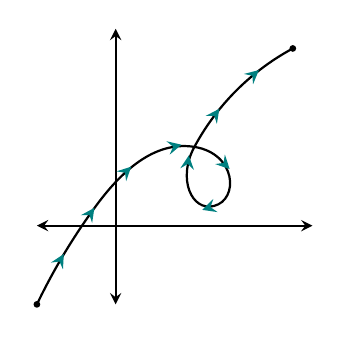
\begin{tikzpicture}[scale=0.5]
    \draw[<->,thick] (-2,0)--(5,0);
	\draw[<->,thick] (0,-2)--(0,5);
    \begin{scope}
        \node(A) at (-2,-2) {};
        \node(B) at (4.5,4.5){};
        \draw[use Hobby shortcut,clockwise arrows,thick]
	(4.5,4.5) .. (2,2) .. (2.5,0.5) .. (2,2) .. (-0.5,0.5) .. (-2,-2);
    \end{scope}
    \draw [fill=black] (A) circle (2pt);
    \draw [fill=black] (B) circle (2pt);
\end{tikzpicture}\]
\begin{center}
\emph{a not simple arc}
\end{center}
\end{minipage}
\begin{minipage}{0.33\textwidth}
\[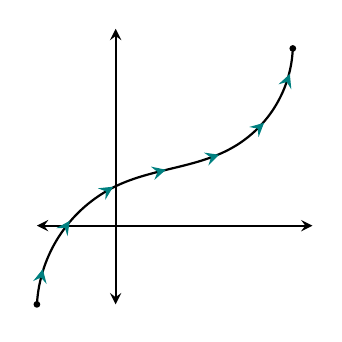
\begin{tikzpicture}[scale=0.5]
    \draw[<->,thick] (-2,0)--(5,0);
	\draw[<->,thick] (0,-2)--(0,5);
    \begin{scope}
        \node(A) at (-2,-2) {};
        \node(B) at (4.5,4.5){};
        \draw[use Hobby shortcut,clockwise arrows,thick]
	(4.5,4.5) .. (3,2) .. (0,1) .. (-2,-2);
    \end{scope}
    \draw [fill=black] (A) circle (2pt);
    \draw [fill=black] (B) circle (2pt);
\end{tikzpicture}\]
\begin{center}
\emph{a simple arc}
\end{center}
\end{minipage}

\bigskip

\begin{minipage}{0.325\textwidth}
\[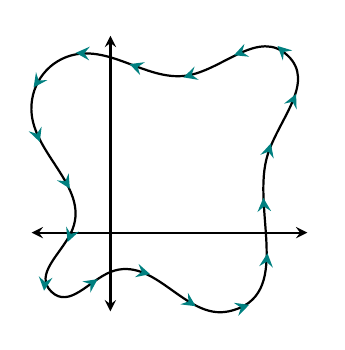
\begin{tikzpicture}[scale=0.5]
    \draw[<->,thick] (-2,0)--(5,0);
	\draw[<->,thick] (0,-2)--(0,5);
    \begin{scope}
        \draw[use Hobby shortcut,closed=true,wise arrows,thick]
	(4.5,4.5) .. (4,2) .. (3,-2) .. (0,-1) .. (-1.5,-1.5) .. (-1,0) .. (-2,3) .. (-1,4.5) .. (2,4) .. (4.5,4.5);
    \end{scope}
\end{tikzpicture}\]
\begin{center}
\emph{a simple closed curve\\ with positive orientation}
\end{center}
\end{minipage}
\begin{minipage}{0.325\textwidth}
\[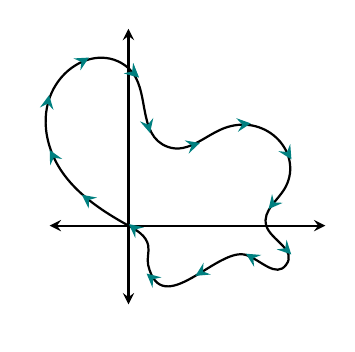
\begin{tikzpicture}[scale=0.5]
    \draw[<->,thick] (-2,0)--(5,0);
	\draw[<->,thick] (0,-2)--(0,5);
    \begin{scope}
        \draw[use Hobby shortcut,closed=true,wise arrows,thick]
	(0,4) .. (-2,2) .. (0,0) .. (0.5,-0.5) .. (0.5,-1) .. (3,-0.75) .. (4,-1) .. (3.5,0) .. (4,1) .. (2.5,2.5) .. (1,2) .. (0,4);
    \end{scope}
\end{tikzpicture}\]
\begin{center}
\emph{a simple closed curve\\ with negative orientation}
\end{center}
\end{minipage}
\begin{minipage}{0.325\textwidth}
\[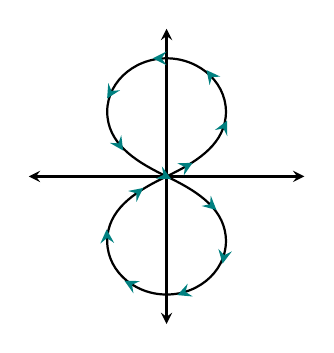
\begin{tikzpicture}[scale=0.5]
    \draw[<->,thick] (-3.5,0)--(3.5,0);
	\draw[<->,thick] (0,-3.75)--(0,3.75);
    \begin{scope}
        \draw[use Hobby shortcut,closed=true,wiser arrows,thick]
	(0,3) .. (1.5,1.5) .. (0,0) .. (-1.5,-1.5) .. (0,-3) .. (1.5,-1.5) .. (0,0) .. (-1.5,1.5) .. (0,3);
    \end{scope}
\end{tikzpicture}\]
\begin{center}
\emph{a not simple closed\\ non-orientable curve}
\end{center}
\end{minipage}
\end{center}

\medskip

\begin{example}
\lecmargin{20}
The most frequently encountered arcs and curves are line segments and circles. 
\begin{itemize}
\item[(1)] The circle of radius $R$ centered at $z_0$ with positive orientation has as a parametrisation
\[z(t) = z_0 + Re^{it},\quad t \in [0,2\pi]\]
\[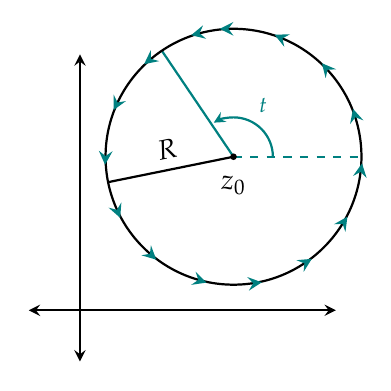
\begin{tikzpicture}[scale=0.65]
    \draw[<->,thick] (-1,0)--(5,0);
	\draw[<->,thick] (0,-1)--(0,5);
    \node (a) at (2,4.732) {};
    \node (b) at (3,3) {};
    \node (c) at (5,3) {};
    \draw pic["{\footnotesize$t$}", ->,>=stealth,thick,draw, angle eccentricity=1.5, angle radius=0.5cm,teal] {angle=c--b--a};
	\draw [teal,dashed,thick] (3,3) -- (5.5,3);
	\draw [teal,thick] (3,3) -- (1.6,5.071);
	\draw [thick] (3,3) -- (0.55,2.503)node [midway,above,sloped] {$R$};
    \node[label=below:$z_0$](A) at (3,3) {};
	\draw [fill=black] (A) circle (1.5pt);
    \begin{scope}
        \draw[use Hobby shortcut,closed=true,wise arrows,thick]
	(3,5.5) .. (5.5,3) .. (3,0.5) .. (0.5,3);
    \end{scope}
\end{tikzpicture}\]

\item[(2)] The circle of radius $R$ centered at $z_0$ with negative orientation has as a parametrisation
\[z(t) = z_0 + Re^{-it},\quad t \in [0,2\pi]\]\\[-1em]
\[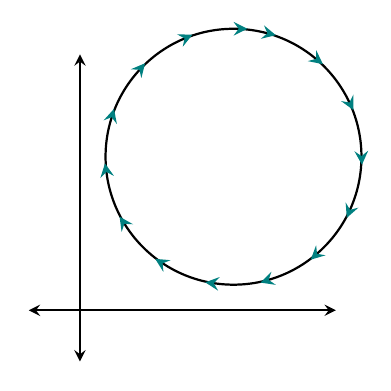
\begin{tikzpicture}[scale=0.65]
    \draw[<->,thick] (-1,0)--(5,0);
	\draw[<->,thick] (0,-1)--(0,5);
    \begin{scope}
        \draw[use Hobby shortcut,closed=true,wise arrows,thick]
	(3,5.5) .. (0.5,3) .. (3,0.5) .. (5.5,3);
    \end{scope}
\end{tikzpicture}\]

\item[(3)] The line segment from $z_0$ to $z_1$ in $\cc$ has as a parametrisation
\[z(t) = z_0 + (z_1 - z_0)t = (1-t)z_0 + tz_1,\quad t \in [0,1]\]\\[-1em]
\[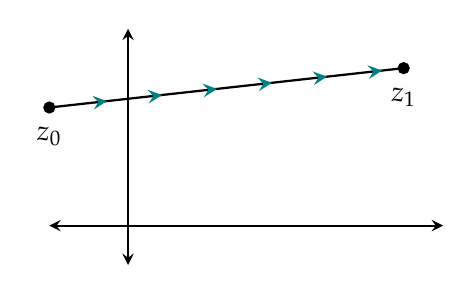
\begin{tikzpicture}
    \draw[<->,thick] (-1,1.5)--(4,1.5);
	\draw[<->,thick] (0,1)--(0,4);
	\begin{scope}
        \draw[use Hobby shortcut,clockwise arrows,thick]
	(3.5,3.5) .. (-1,3);
    \end{scope}    
    \node[label=below:$z_0$](A) at (-1,3) {};
    \node[label=below:$z_1$](B) at (3.5,3.5){};
	\draw [fill=black] (A) circle (2pt);
    \draw [fill=black] (B) circle (2pt);
\end{tikzpicture}\]
\end{itemize}
\end{example}

\medskip

\begin{definition}[Reparametrisation of an arc]
Suppose an arc $C$ is parametrised by $z:[a,b] \to \cc$. A map
\[w:[c,d] \to \cc\]
is called an \cdef{orientation\text{-}preserving\ reparametrisation} of $C$ if there exists a surjective function
\[\phi:[c,d] \to [a,b]\]
with continuous derivative such that $\phi(c) = a$ (preserves initial point), $\phi(d) = b$ (preserves final point), $\phi'(s) > 0$ and $w(s) = z(\phi(s))$ ($w$ and $z$ trace out the same arc $C$).
\end{definition}

\medskip

\begin{example}
Note that $z(t) = e^{it}$ for $t \in [0,2\pi]$ is a parametrisation of the unit circle. Now, consider
\[w:[0,\pi] \to \cc,\ s \mapsto e^{2is},\]
this is, in fact, an orientation-preserving reparametrisation of the unit circle. To conclude this, we produce the following surjective map
\[\phi:[0,\pi] \to [0,2\pi],\ s \mapsto 2s,\]
we note that $\phi(0) = 0$ and $\phi(\pi) = 2\pi$, furthermore $\phi'(s) = 2 > 0$ which is clearly continuous. Lastly, $z(\phi(s)) = z(2s) = e^{2is} = w(s)$.
\end{example}

\medskip

\begin{remark}
Suppose an arc $C$ is parametrised by $z:[a,b] \to \cc$, a map $w:[c,d] \to \cc$ 
is called an \cdef{orientation\text{-}reversing\ reparametrisation} of $C$ if there exists a surjective function
\[\psi:[c,d] \to [a,b]\]
with continuous derivative such that $\psi(c) = b$ and $\psi(d) = b$ (swaps initial and final points), $\psi'(s) < 0$ and $w(s) = z(\psi(s))$ ($w$ and $z$ trace out the same arc $C$).\\
\\
Consider the unit circle, which has parametrisation $z(t) = e^{it},\ t \in [0,2\pi]$. Then $w(t) = e^{-it}$ for $0 \leq t \leq 2\pi$ is an orientation-reversing parametrisation. To see this, we consider the surjective function
\[\psi:[0,2\pi] \to [0,2\pi],\ s \mapsto 2\pi - s;\]
we note that $\psi(0) = 2\pi$ and $\psi(2\pi) = 0$, furthermore $\psi'(s) = -1 < 0$ and \[z(\psi(s)) = z(2\pi - s) = e^{2\pi i - is} = e^{-is} = w(s),\] since $e^{2\pi i} = 1$.
\end{remark}

\medskip

\begin{definition}[Arc length and Smooth arcs]\hfill
\begin{itemize}
\item[(1)] If $C$ is parametrised by $z(t) = x(t) + iy(t)$ and $x'(t),\,y'(t)$ exist and are continuous on $[a,b]$, then $C$ is called a \cdef{differentiable\ arc}.
\item[(2)] The \cdef{arc\ length} of such a differentiable arc $C$ is
\[L(C) = \int_a^b \abs{z'(t)}\,dt = \int_a^b\sqrt{x'(t)^2 + y'(t)^2}\,dt\]
\item[(3)] A differentiable curve parametrised by $z(t)$ is called \cdef{smooth} if $z'(t) \neq 0$ on $[a,b]$.
\end{itemize}
\end{definition}

\medskip

\begin{definition}[Contours]
A \cdef{contour} is an arc consisting of a finite number of smooth arcs joined end to end.\\[0.5em]
A \cdef{simple\ closed\ contour} is a contour that does not cross itself except that the initial and final points are the same.
\end{definition}

\medskip

\begin{discussion}[Jordan Curve Theorem]
A deep theorem known as the \emph{Jordan Curve theorem} tells us that every simple closed contour $C$ is the boundary of two distinct domains called the \cdef{interior\ of} {\color{darkred}$C$}, which is bounded, and the \cdef{exterior\ of} {\color{darkred}$C$}, which is unbounded.
\[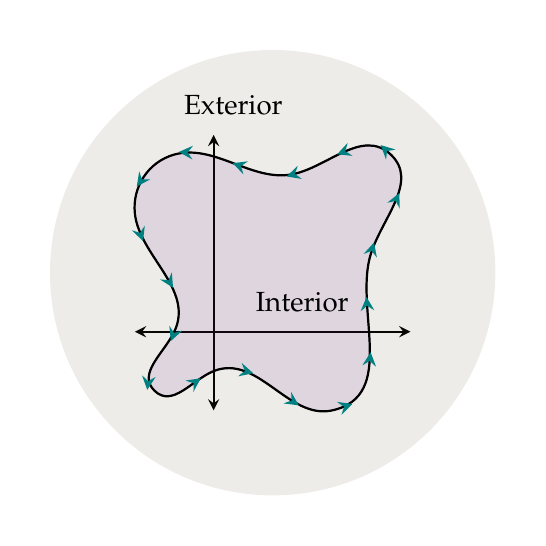
\begin{tikzpicture}[scale=0.5]
    \draw[<->,thick] (-2,0)--(5,0);
	\draw[<->,thick] (0,-2)--(0,5);
    \begin{scope}
    \draw[use Hobby shortcut,closed=true,fill=dirt,fill opacity=0.1,draw opacity=0]
	(5.5,5.5) .. (-2.5,5.5) .. (-2.5,-2.5) .. (5.5,-2.5) .. (5.5,5.5);
    \draw[use Hobby shortcut,closed=true,wise arrows,fill=indigo,fill opacity=1/10]
	(4.5,4.5) .. (4,2) .. (3,-2) .. (0,-1) .. (-1.5,-1.5) .. (-1,0) .. (-2,3) .. (-1,4.5) .. (2,4) .. (4.5,4.5);
    \draw[use Hobby shortcut,closed=true,wise arrows,thick]
	(4.5,4.5) .. (4,2) .. (3,-2) .. (0,-1) .. (-1.5,-1.5) .. (-1,0) .. (-2,3) .. (-1,4.5) .. (2,4) .. (4.5,4.5);
    \end{scope}
    \node[label=below:{Interior}](A) at (2.25,1.5) {};
    \node[label=below:{Exterior}](B) at (0.5,6.5) {};
\end{tikzpicture}\]

The theorem is geometrically evident but the proof is not easy. We will assume its truth so that we can refer to the interior of a simple closed contour.
\end{discussion}

\bigskip

\subsection{Contour Integration}
%\begin{mdframed}
%\begin{center}
%{\Large Contour Integration}
%\end{center}
%\end{mdframed}

\begin{definition}[Contour Integral]
Suppose $f:G \to \cc$ is a complex function and $C$ is a contour lying in $G$. If $z(t)$, $t \in [a,b]$, is a parametrisation of $C$ and $f(z(t))$ is piecewise continuous, then the \cdef{contour\ integral\ of} {\color{darkred}$f$} \cdef{over} {\color{darkred}$C$} is
\[\int_C\, f(z)\ dz \coloneqq \int_a^b f(z(t))\,z'(t)\ dt\]
\begin{remark}
As $C$ is a contour, $z'(t)$ is piecewise continuous and thus the above integral exists.
\end{remark}
\end{definition}

\medskip

\begin{proposition}[Integral is parametrisation-independent]
Suppose $z:[a,b] \to \cc$ parametrises $C$ and $w:[c,d] \to \cc$ is an orientation-preserving reparametrisation of $C$, then
\[\int_C\,f(z)\ dz = \int_C\, f(w)\ dw\]
\end{proposition}
\begin{proof}
By definition of an orientation-preserving reparametrisation, there exists a surjective map $\phi:[c,d] \to [a,b]$ such that $\phi(c) = a,\,\phi(d) = b,\, \phi'(s) > 0$ and $w(s) = \phi(z(s))$. Then
\begin{align*}
\int_C\, f(w)\ dw &= \int_c^d f(w(s))\,w'(s)\ ds\\[0.5em]
 &= \int_c^d f(z(\phi(s)))\,\phi'(z(s))\,z'(s)\ ds && \text{apply chain rule to $w(s) = \phi(z(s))$}\\[0.5em]
 &= \int_a^b f(z(t))\,z'(t)\ dt && \text{set $t = \phi(s)$}\\[0.5em]
 &= \int_C\, f(z)\ dz
\end{align*}
\end{proof}

\medskip

\begin{discussion}[Notation for Contours]\hfill\lecmargin{21}
\begin{itemize}[itemsep=2em]
\item[(1)] Suppose $C$ is a contour, then $-C$ denotes the same set of points as $C$ but with opposite orientation. If $z:[a,b] \to \cc$ is a parametrisation of $C$, then $w:[-b,-a] \to \cc$ defined as $w(t) \coloneqq z(-t)$ is a parametrisation of $-C$.
\[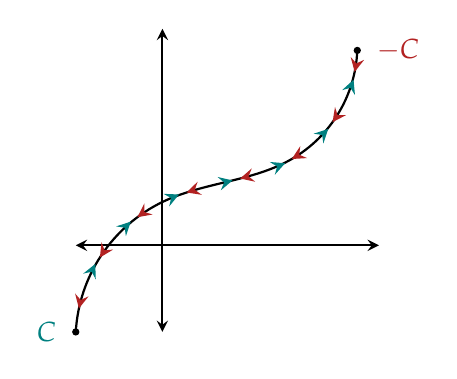
\begin{tikzpicture}[scale=0.55]
    \draw[<->,thick] (-2,0)--(5,0);
	\draw[<->,thick] (0,-2)--(0,5);
    \begin{scope}
        \node[label=left:{\color{teal}$C$}](A) at (-2,-2) {};
        \node[label=right:{\color{firebrick}$-C$}](B) at (4.5,4.5) {};
        \draw[use Hobby shortcut,counterclockwise arrows,clockwise arrows,thick]
	(4.5,4.5) .. (3,2) .. (0,1) .. (-2,-2);
    \end{scope}
    \draw [fill=black] (A) circle (2pt);
    \draw [fill=black] (B) circle (2pt);
\end{tikzpicture}\]
\item[(2)] If $C_1$ is a contour from $z_1$ to $z_2$ and $C_2$ is a contour from $z_2$ to $z_3$, then their \cdef{sum} $C = C_1 + C_2$ is the contour obtained by transversing $C_1$ and then $C_2$.

\begin{center}
\begin{minipage}{0.4\textwidth}
\[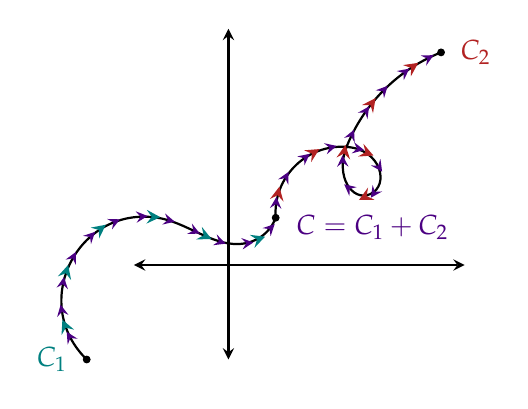
\begin{tikzpicture}[scale=0.6]
    \draw[<->,thick] (-2,0)--(5,0);
	\draw[<->,thick] (0,-2)--(0,5);
    \begin{scope}
        \node[label=left:{\color{teal}$C_1$}](A) at (-3,-2) {};
        \node[label={[xshift=3.5em,yshift=-1.5em]\color{indigo}$C = C_1 + C_2$}](B) at (1,1){};
        \node[label=right:{\color{firebrick}$C_2$}](C) at (4.5,4.5){};
        \draw[use Hobby shortcut,clockwise arrows, clockwise arrowsmore,thick]
	(1,1) .. (0.5,0.5) .. (-1.5,1) .. (-3,-2);
        \draw[use Hobby shortcut,clockwise arrowsnew, clockwise arrowsmore,thick]
	(4.5,4.5) .. (2.5,2.5) .. (3,1.5) .. (2.5,2.5) .. (1,1);
    \end{scope}
    \draw [fill=black] (A) circle (2pt);
    \draw [fill=black] (B) circle (2pt);
    \draw [fill=black] (C) circle (2pt);
\end{tikzpicture}\]
\end{minipage} \hspace*{2em} 
\begin{minipage}{0.4\textwidth}
\[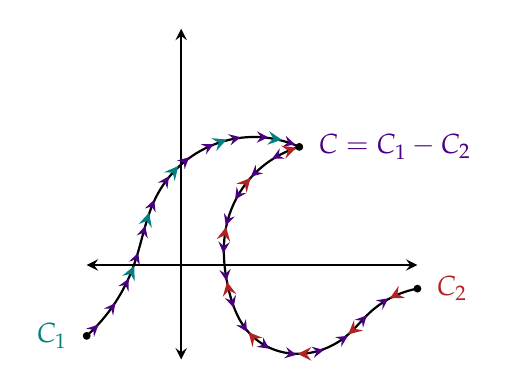
\begin{tikzpicture}[scale=0.6]
    \draw[<->,thick] (-2,0)--(5,0);
	\draw[<->,thick] (0,-2)--(0,5);
    \begin{scope}
        \node[label=left:{\color{teal}$C_1$}](A) at (-2,-1.5) {};
        \node[label=right:{\color{indigo}$C = C_1 - C_2$}](B) at (2.5,2.5){};
        \node[label=right:{\color{firebrick}$C_2$}](C) at (5,-0.5){};
        \draw[use Hobby shortcut,clockwise arrows, clockwise arrowsmore,thick]
	(2.5,2.5) .. (-0.5,1.5) .. (-1,0) .. (-2,-1.5);
        \draw[use Hobby shortcut,counterclockwise arrows2, clockwise arrowsmorenew,thick]
	(5,-0.5) .. (4,-1) .. (3.5,-1.5) .. (1.5,-1.5) .. (1,-0.5) .. (1,1) .. (2.5,2.5);
    \end{scope}
    \draw [fill=black] (A) circle (2pt);
    \draw [fill=black] (B) circle (2pt);
    \draw [fill=black] (C) circle (2pt);
\end{tikzpicture}\]
\end{minipage}
\end{center}

If $C_1$ and $C_2$ have the same final point, then we can consider the sum of $C_1$ and $-C_2$ and is written as $C_1 - C_2 \coloneqq C_1 + (-C_2)$.
\end{itemize}
\end{discussion}

\medskip

\begin{proposition}[Properties of Contour Integral]\label{contprop}
Assume $f,\,g$ are piecewise continuous on the contours we consider below.
\begin{itemize}[itemsep=1em]
\item[(1)] $\displaystyle \int_C\,z_0 f(z)\ dz = z_0\int_C\, f(z)\ dz$, for any $z_0 \in \cc$.
\item[(2)] $\displaystyle \int_C\, f(z) + g(z)\ dz = \int_C\, f(z)\ dz + \int_C g(z)\ dz$.
\item[(3)] $\displaystyle \int_{-C}\, f(z)\ dz = -\int_C\,f(z)\ dz$.
\item[(4)] $\displaystyle \int_C\, f(z)\ dz = \int_{C_1}\, f(z)\ dz + \int_{C_2}\, f(z)\ dz$ if $C = C_1 + C_2$.
\end{itemize}
\end{proposition}
\begin{proof}\hfill
\begin{itemize}
\item[(1)] Suppose $C$ is parametrised by $z:[a,b] \to \cc$
\begin{align*}
\int_C\,z_0 f(z)\ dz &=  \int_C\,z_0 f(z(t))\,z'(t)\ dz\\[0.5em]
&=  z_0\int_a^b\, f(z(t))\,z'(t)\ dz && \text{by Proposition \ref{paraint} (1)}\\[0.5em]
&=  z_0\int_C\, f(z)\ dz
\end{align*}
\item[(2)] This will follow from Proposition \ref{paraint} (2).
\item[(3)] Suppose $C$ is parametrised by $z:[a,b] \to \cc$, then, as we note before, a parametrisation of $-C$ is $w:[-b,-a] \to \cc$ where $w(t) = z(-t)$. Then
\begin{align*}
\int_{-C}\,f(w)\ dw &= \int_{-b}^{-a}\, f(w(t))\,w'(t)\ dt\\[0.5em]
 &= -\int_{-b}^{-a}\, f(z(-t))\,z'(-t)\ dt && \text{apply chain rule to $w(t) = z(-t)$}\displaybreak\\[0.5em]
 &= -\int_{-a}^{-b}\, f(z(-t))\,z'(-t)\ dt && \text{by Proposition \ref{paraint} (4)}\\[0.5em]
 &= \int_{a}^{b}\, f(z(s))\,z'(s)\ ds && \text{set $s=-t$}\\[0.5em]
 &= \int_C\, f(z)\ dz
\end{align*}
\item[(4)] We leave this as an exercise for the motivated student.
\end{itemize}
\vspace*{-\baselineskip}
\end{proof}

\medskip

\begin{example}\hfill
\begin{itemize}[itemsep=1.5em]
\item[(1)] Integrate $f(z) = \dfrac{1}{z}$ over the following contours:
\begin{itemize}
\item[$\bullet$] $C_1$: upper semicircle of the unit circle, from $1$ to $-1$.
\item[$\bullet$] $C_2$: lower semicircle of the unit circle, from $1$ to $-1$.
\item[$\bullet$] $C_3$: $C_1 - C_2$.
\end{itemize}
\begin{minipage}{0.6\textwidth}
For $C_1$, parametrise $C_1$ as $z(t) = e^{it},\ 0 \leq t \leq \pi$. Then
\[\int_{C_1}\,\frac{1}{z}\ dz = \int_0^\pi \frac{1}{e^{it}}\, ie^{it}\ dt = i\int_0^\pi\,dt = \pi i\]
\end{minipage}
\begin{minipage}{0.3\textwidth}
\[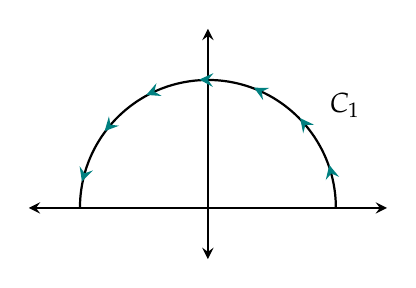
\begin{tikzpicture}[scale=1.3]
    \draw[<->,thick] (-1.75,0)--(1.75,0);
	\draw[<->,thick] (0,-0.5)--(0,1.75);
    \begin{scope}
        \node[label=right:{$C_1$}](A) at (1,1) {};
        \draw[use Hobby shortcut,clockwise arrows,thick]
	(-1.25,0) .. (0,1.25) .. (1.25,0);
    \end{scope}
\end{tikzpicture}\]
\end{minipage}

\medskip

\begin{minipage}{0.6\textwidth}
For $C_2$, parametrise $C_2$ as $z(t) = e^{-it},\ 0 \leq t \leq \pi$. Then
\[\int_{C_1}\,\frac{1}{z}\ dz = \int_0^\pi \frac{1}{e^{-it}}\, (-ie^{-it})\ dt = -i\int_0^\pi\,dt = -\pi i\]
\end{minipage}
\begin{minipage}{0.3\textwidth}
\[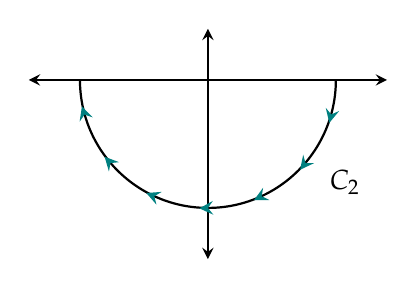
\begin{tikzpicture}[scale=1.3]
    \draw[<->,thick] (-1.75,0)--(1.75,0);
	\draw[<->,thick] (0,-1.75)--(0,0.5);
    \begin{scope}
        \node[label=right:{$C_2$}](A) at (1,-1) {};
        \draw[use Hobby shortcut,clockwise arrows,thick]
	(-1.25,0) .. (0,-1.25) .. (1.25,0);
    \end{scope}
\end{tikzpicture}\]
\end{minipage}

\medskip

\begin{minipage}{0.6\textwidth}
Note
\begin{align*}
\int_{C_3}\,\frac{1}{z}\ dz = \int_{C_1 - C_2}\,\frac{1}{z}\ dz &= \int_{C_1}\,\frac{1}{z}\ dz + \int_{- C_2}\,\frac{1}{z}\ dz\\[0.5em]
 &= \int_{C_1}\,\frac{1}{z}\ dz - \int_{C_2}\,\frac{1}{z}\ dz\\[0.5em]
 &= \pi i - (-\pi i)\\[0.5em]
 &= 2\pi i
\end{align*}
\end{minipage}
\begin{minipage}{0.3\textwidth}
\[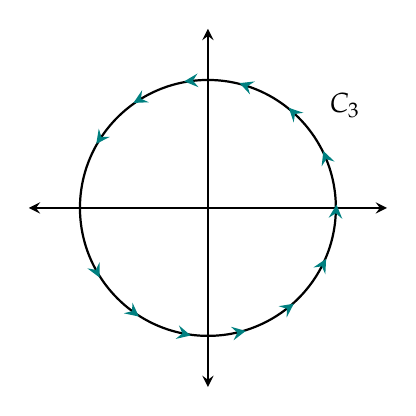
\begin{tikzpicture}[scale=1.3]
    \draw[<->,thick] (-1.75,0)--(1.75,0);
	\draw[<->,thick] (0,-1.75)--(0,1.75);
    \begin{scope}
        \node[label=right:{$C_3$}](A) at (1,1) {};
        \draw[use Hobby shortcut,clockwise arrows,thick]
	(-1.25,0) .. (0,1.25) .. (1.25,0) .. (0,-1.25) .. (-1.25,0);
    \end{scope}
\end{tikzpicture}\]
\end{minipage}

\emph{This example shows that the integral may depend on the path taken and not just on the endpoints. Also, the integral over a closed contour may be non-zero.}

\item[(2)] Integrate $f(z) = z$ over \emph{any} contour $C$ connecting a point $w_1$ to a point $w_2$.\\[0.5em]
First, suppose $C$ is a smooth arc joining $w_1$ and $w_2$ with parametrisation $z:[a,b] \to \cc$.
\[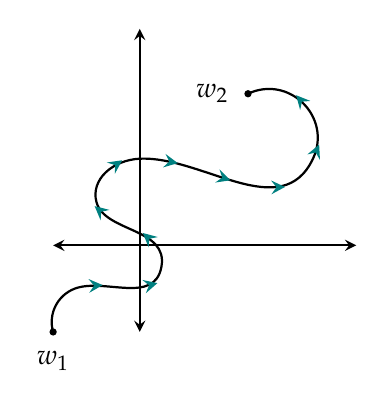
\begin{tikzpicture}[scale=0.55]
    \draw[<->,thick] (-2,0)--(5,0);
	\draw[<->,thick] (0,-2)--(0,5);
    \begin{scope}
        \node[label=below:{$w_1$}](A) at (-2,-2) {};
        \node[label=left:{$w_2$}](B) at (2.5,3.5) {};
        \draw[use Hobby shortcut,clockwise arrows,thick]
	(2.5,3.5) .. (4,2) .. (0,2) .. (-1,1) .. (0.5,-0.5) .. (-1.5,-1) .. (-2,-2);
    \end{scope}
    \draw [fill=black] (A) circle (2pt);
    \draw [fill=black] (B) circle (2pt);
\end{tikzpicture}\]
Since,\[\left(\frac{z(t)^2}{2}\right)' = \frac{z'(t)z(t) + z(t)z'(t)}{2} = z(t)z'(t).\]
Therefore,
\begin{align*}
\int_C\,f(z)\ dz = \int_C\,z\ dz &= \int_a^b\,z(t)\,z'(t)\ dt\\[0.5em]
 &= \frac{z(b)^2}{2} - \frac{z(a)^2}{2},\ \text{by Proposition \ref{pathftc}}\\[0.5em]
 &= \frac{w_2^2 - w_1^2}{2}
\end{align*}

%\begin{minipage}{0.6\textwidth}
%Since,\[\left(\frac{z(t)^2}{2}\right)' = \frac{z'(t)z(t) + z(t)z'(t)}{2} = z(t)z'(t).\]
%Therefore,
%\begin{align*}
%\int_C\,f(z)\ dz = \int_C\,z\ dz &= \int_a^b\,z(t)\,z'(t)\ dt\\[0.5em]
% &= \frac{z(b)^2}{2} - \frac{z(a)^2}{2},\ \text{by Proposition \ref{pathftc}}\\[0.5em]
% &= \frac{w_2^2 - w_1^2}{2}
%\end{align*}
%\end{minipage}\hspace*{1em}
%\begin{minipage}{0.3\textwidth}
%\[\begin{tikzpicture}[scale=0.5]
%    \draw[<->,thick] (-2,0)--(5,0);
%	\draw[<->,thick] (0,-2)--(0,5);
%    \begin{scope}
%        \node[label=below:{$w_1$}](A) at (-2,-2) {};
%        \node[label=left:{$w_2$}](B) at (2.5,3.5) {};
%        \draw[use Hobby shortcut,clockwise arrows,thick]
%	(2.5,3.5) .. (4,2) .. (0,2) .. (-1,1) .. (0.5,-0.5) .. (-1.5,-1) .. (-2,-2);
%    \end{scope}
%    \draw [fill=black] (A) circle (2pt);
%    \draw [fill=black] (B) circle (2pt);
%\end{tikzpicture}\]
%\end{minipage}

\medskip

Now, if $C$ is a contour, we can write $C = C_1 + \cdots + C_n$, where $C_i$ is a smooth arc joining $z_i$ to $z_{i+ 1}$ with $z_1 = w_1$ and $z_{n+1} = w_2$. Then,
\begin{align*}
\int_C\,z\ dz &= \sum_{i=1}^n\int_{C_i}\,z\ dz,\ \text{by Proposition \ref{contprop} (4)}\\[0.5em]
 &= \sum_{i=1}^n \frac{z_{i+1}^2 - z_i^2}{2}\\[0.5em]
 &= \frac{z_{n+1}^2 - z_1^2}{2}\\[0.5em]
 &= \frac{w_2^2 - w_1^2}{2}
\end{align*}

\emph{This example shows that some integrals do depend only on the end points and not the path taken. Also, for any contour $C$ is closed, that is, when $w_2 = w_1$, we have shown hence that
\[\int_C z\ dz = 0.\]}

\item[(3)] Integrate $f(z) = z^m\overline{z}^n$, for $m,n \in \zz$, over the unit circle $C$.
\[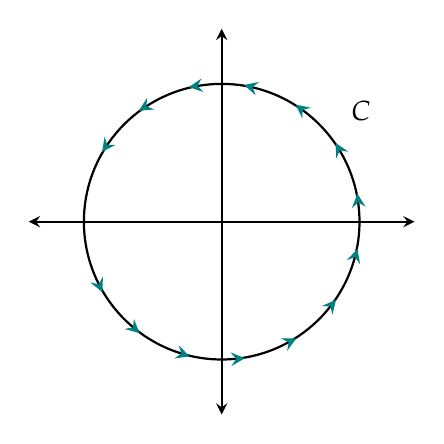
\begin{tikzpicture}[scale=1.4]
    \draw[<->,thick] (-1.75,0)--(1.75,0);
	\draw[<->,thick] (0,-1.75)--(0,1.75);
    \begin{scope}
        \node[label=right:{$C$}](A) at (1,1) {};
        \draw[use Hobby shortcut,clockwise arrows,thick]
	(-1.25,0) .. (0,1.25) .. (1.25,0) .. (0,-1.25) .. (-1.25,0);
    \end{scope}
\end{tikzpicture}\]
Parametrise $C$ as $z(t) = e^{it},\ 0 \leq t \leq 2\pi$. Then,
\begin{align*}
\int_C\,f(z)\ dz &= \int_C\,z^m\overline{z}^n\ dz\\[0.5em]
 &= \int_0^{2\pi}\,(e^{it})^m(\overline{e^{it}})^n\,ie^{it}\ dt\\[0.5em]
 &= i\int_0^{2\pi}\,(e^{it})^m(e^{-it})^n\,e^{it}\ dt\\[0.5em]
 &= i\int_0^{2\pi}\,e^{imt}e^{-int}e^{it}\ dt\\[0.5em]
 &= i\int_0^{2\pi}\,e^{(m - n + 1)it}\ dt
\end{align*}

\medskip
\noindent
Case I.\ $m = n-1$
\[\int_C\,f(z)\ dz = i\int_0^{2\pi}\,e^{(m - n + 1)it} = i\int_0^{2\pi}\ dt = 2\pi i\]\\
Case II.\ $m \neq n-1$
\begin{align*}
\int_C\,f(z)\ dz = i\int_0^{2\pi}\,e^{(m - n + 1)it} &= i\Bigg[\frac{e^{(m - n + 1)it}}{i(m - n + 1)}\Bigg]_0^{2\pi}\\[0.5em]
 &= \frac{1}{m - n + 1}\left(e^{2(m - n + 1)\pi i} - e^0\right)\\[0.5em]
 &= \frac{1}{m - n + 1}\,(1 - 1)\\[1em]
 &= 0
\end{align*}
%\begin{minipage}{0.6\textwidth}
%Parametrise $C$ as $z(t) = e^{it},\ 0 \leq t \leq 2\pi$. Then,
%\begin{align*}
%\int_C\,f(z)\ dz = \int_C\,z^m\overline{z}^n\ dz &= \int_0^{2\pi}\,(e^{it})^m(\overline{e^{it}})^n\,ie^{it}\ dt\\[0.5em]
% &= i\int_0^{2\pi}\,(e^{it})^m(e^{-it})^n\,e^{it}\ dt\\[0.5em]
% &= i\int_0^{2\pi}\,e^{imt}e^{-int}e^{it}\ dt\\[0.5em]
% &= i\int_0^{2\pi}\,e^{(m - n + 1)it}\ dt\\[1em]
%\text{Case I.\ $m = n-1$}\\[0.5em]
% &= i\int_0^{2\pi}\ dt\\[0.5em]
% &= 2\pi i\\[1em]
%\text{Case II.\ $m \neq n-1$}\\[0.5em]
% &= i\Bigg[\frac{e^{(m - n + 1)it}}{i(m - n + 1)}\Bigg]_0^{2\pi}\\[0.5em]
% &= \frac{1}{m - n + 1}\left(e^{2(m - n + 1)\pi i} - e^0\right)\\[0.5em]
% &= \frac{1}{m - n + 1}\,(1 - 1)\\[0.5em]
% &= 0
%\end{align*}
%\end{minipage}\hspace*{1em}
%\begin{minipage}{0.3\textwidth}
%
%\end{minipage}
\end{itemize}

\medskip

Some examples involving a branch of a multi-valued function.\lecmargin{22}
\begin{itemize}[itemsep=1.5em]
\item[(4)] Integrate the branch of square root \[f(z) = z^{1/2} = e^{(1/2)\log z},\quad \abs{z}>0,\ 0 < \arg z < 2\pi\] over the contour
\[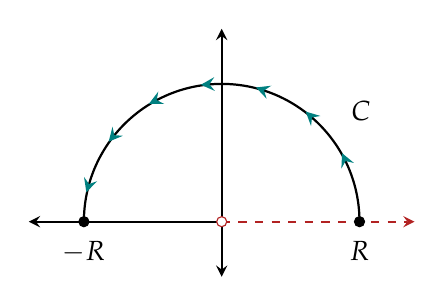
\begin{tikzpicture}[scale=1.4]
    \draw[<-,thick] (-1.75,0)--(0,0);
	\draw[<->,thick] (0,-0.5)--(0,1.75);
    \begin{scope}
        \node[label=right:{$C$}](A) at (1,1) {};
        \node[label=below:{$-R$}](B) at (-1.25,0) {};
        \node[label=below:{$R$}](C) at (1.25,0) {};
        \draw[use Hobby shortcut,clockwise arrows,thick]
	(-1.25,0) .. (0,1.25) .. (1.25,0);
    \end{scope}
	\draw[->,thick,dashed,firebrick] (0,0)--(1.75,0);
    \draw [firebrick,fill=white] (0,0) circle (1.3pt);
    \draw [fill=black] (B) circle (1.3pt);
    \draw [fill=black] (C) circle (1.3pt);
\end{tikzpicture}\]
\[C:\ z(t) = Re^{it},\quad R>0,\ 0 \leq t \leq \pi\]
Note that $f(z)$ is not defined at the initial point $z = R$ of the contour $C$ as $\arg R = 0$, that is, $f(z(t))$ is not defined for $t = 0$. The integral
\[\int_C\,f(z)\ dz = \int_0^{\pi}\,f(z(t))\,z'(t)\ dt\]
nevertheless exists as the integrand $f(z(t))\,z'(t)$ is piecewise continuous on $[0,\pi]$. To see this, we note that for $0 < t \leq \pi$
\allowdisplaybreaks
\begin{align*}
f(z(t))\,z'(t) = e^{(1/2)\log Re^{it}}Rie^{it} &= iRe^{(\ln R + it)/2}e^{it}\\[0.5em]
 &= iR(R^{1/2}e^{it/2})e^{it}\\[0.5em]
 &= iR^{3/2}e^{3it/2}\\[0.5em]
 &= iR^{3/2}\left(\cos\frac{3t}{2} + i\sin\frac{3t}{2}\right) = R^{3/2}\left(-\sin\frac{3t}{2} + i\cos\frac{3t}{2}\right)
\end{align*}
The right hand limits of the real and imaginary parts of $f(z(t))\,z'(t)$ at $t = 0$ exist, and equal $0$ and $R^{3/2}$. Therefore, $f(z(t))\,z'(t)$ is continuous on $[0,\pi]$ with its value at $t = 0$ defined as $iR^{3/2}$. Hence, 
\begin{align*}
\int_C\,f(z)\ dz = \int_0^{\pi}\,f(z(t))\,z'(t)\ dt &= \int_0^{\pi}\,iR^{3/2}e^{3it/2}\ dt\\[0.5em]
&= iR^{3/2}\int_0^{\pi}\,e^{3it/2}\ dt\\[0.5em]
&= iR^{3/2}\Bigg[\frac{e^{3it/2}}{3i/2}\Bigg]_0^{\pi}\\[0.5em]
&= \frac{2}{3}R^{3/2}\left(e^{3\pi i/2} - e^0\right)\\[0.5em]
&= \frac{2}{3}R^{3/2}\left(-i - 1\right)\\[0.5em]
&= -\frac{2}{3}R^{3/2}\left(1 + i\right)
\end{align*}

\item[(5)] Integrate the principal branch of \[f(z) = z^{i-1} = e^{(i - 1)\plog z},\quad \abs{z}>0,\ -\pi < \parg z < \pi\] over the contour
\[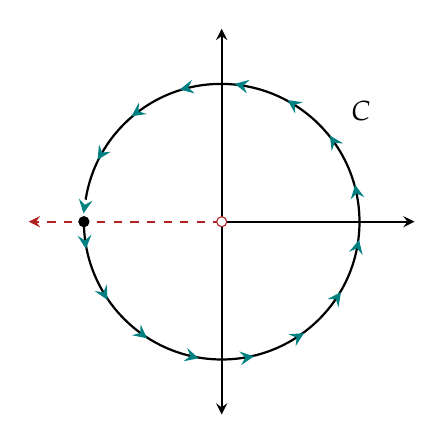
\begin{tikzpicture}[scale=1.4]
    \draw[<-,thick] (1.75,0)--(0,0);
	\draw[<->,thick] (0,1.75)--(0,-1.75);
    \begin{scope}
        \node[label=right:{$C$}](A) at (1,1) {};
        \draw[use Hobby shortcut,clockwise arrowsend,thick]
	(-1.234,0.2) .. (0,1.25) .. (1.25,0) .. (0,-1.25) .. (-1.25,0);
    \end{scope}
	\draw[->,thick,dashed,firebrick] (0,0)--(-1.75,0);
    \draw [fill=black] (-1.25,0) circle (1.3pt);
    \draw [firebrick,fill=white] (0,0) circle (1.3pt);
\end{tikzpicture}\]
\[C:\ z(t) = e^{it},\quad R>0,\ -\pi \leq t \leq \pi\]
Since the curve crosses the branc cut, we need to check if integrand $f(z(t))\,z'(t)$ is piecewise continuous on $[-\pi,\pi]$. To see this, we note that for $-\pi < t \leq \pi$
\begin{align*}
f(z(t))\,z'(t) = e^{(i - 1)\plog e^{it}}ie^{it} &= ie^{(i-1)(\ln 1 + it)}e^{it}\\[0.5em]
 &= ie^{(i-1)it}e^{it}\\[0.5em]
 &= ie^{(i - 1)it + it}\\[0.5em]
 &= ie^{i^2t} = ie^{-t}
\end{align*}
The right hand limits of the real and imaginary parts of $f(z(t))\,z'(t)$ at $t = \pi$ exist, and equal $0$ and $e^{-\pi}$. Therefore, $f(z(t))\,z'(t)$ is continuous on $[-\pi,\pi]$ with its value at $t = -\pi$ defined as $ie^{-\pi}$. Hence, 
\begin{align*}
\int_C\,f(z)\ dz = \int_{-\pi}^{\pi}\,f(z(t))\,z'(t)\ dt &= \int_{-\pi}^{\pi}\,ie^{-t}\ dt\\[0.5em]
&= i\int_{-\pi}^{\pi}\,e^{-t}\ dt\\[0.5em]
&= i\Big[-e^{-t}\Big]_{-\pi}^{\pi}\\[0.5em]
&= i\left(-e^{-\pi} - (-e^{-(-\pi)})\right)\\[0.5em]
&= i\left(e^{\pi}-e^{-\pi}\right)
\end{align*}
\end{itemize}
\end{example}

\bigskip

\subsection{Estimating Contour Integrals}
%\begin{mdframed}
%\begin{center}
%{\Large Estimating Contour Integrals}
%\end{center}
%\end{mdframed}

\begin{lemma}[Triangle Inequality for Integrals]\label{intriineq}
Suppose $\gamma:[a,b] \to \cc$ is piecewise continuous. Then
\[\abs{\int_a^b\,\gamma(t)\ dt} \leq \int_a^b\abs{\gamma(t)}dt\]
\end{lemma}
\begin{proof}
Let's first assume 
\[\int_a^b\,\gamma(t)\ dt = 0,\]
then the lemma holds as $\abs{\gamma(t)} \geq 0$ for all $t \in [a,b]$ and so its integral is non-negative. Otherwise, let \[r_0e^{it_0} = \int_a^b\,\gamma(t)\ dt \neq 0.\] Then,
\begin{align*}
\abs{\int_a^b\,\gamma(t)\ dt} = |r_0e^{it_0}| = r_0 = \Re r_0 &= \Re (r_0e^{it_0}e^{-it_0})\\[0.5em]
&= \Re \left(e^{-it_0}\int_a^b\,\gamma(t)\ dt\right)\\[0.5em]
&= \Re \left(\int_a^b\,e^{-it_0}\gamma(t)\ dt\right)\\[0.5em]
&= \int_a^b\,\Re (e^{-it_0}\gamma(t))\ dt\\[0.5em]
&\leq \int_a^b\,|e^{-it_0}\gamma(t)|\ dt,\ \text{using Discussion \ref{cmplxnorm}}\\[0.5em]
&= \int_a^b\,|e^{-it_0}|\abs{\gamma(t)}\ dt\\[0.5em]
&= \int_a^b\abs{\gamma(t)} dt\\[-3em]
\end{align*}
\end{proof}

\medskip

\begin{theorem}[Bound for Contour Integrals]\label{contourtriineq}
Suppose that $C$ is a contour of length $L$ and $f$ is piecewise continuous on $C$. Then
\[\abs{\int_C\,f(z)\ dz} \leq \max_{z \in C}\abs{f(z)} \cdot L(C)\]
\end{theorem}
\begin{proof}
Suppose $z:[a,b] \to \cc$ parametrises $C$. By assumption $f(z(t))$ is piecewise continuous on $[a,b]$. Hence, $\max_{z \in C}\abs{f(z)} = \max_{t \in [a,b]}\abs{f(z(t))}$ is finite as $f(z(t))$ is continuous on a closed and bounded interval. Thus,
\begin{align*}
\abs{\int_C\,f(z)\ dz} &= \abs{\int_a^b\,f(z(t))\,z'(t)\ dz}\\[0.5em]
 &\leq \int_a^b\abs{f(z(t))\,z'(t)}\, dz,\ \text{by Lemma \ref{intriineq}}\\[0.5em]
 &= \int_a^b\abs{f(z(t))}\abs{z'(t)}\, dz\\[0.5em]
 &\leq \int_a^b\max_{t \in [a,b]}\abs{f(z(t))}\abs{z'(t)}\, dz\\[0.5em]
 &= \max_{t \in [a,b]}\abs{f(z(t))}\int_a^b\abs{z'(t)}\, dz = \max_{t \in [a,b]}\abs{f(z(t))}\cdot L(C) = \max_{z \in C}\abs{f(z)}\cdot L(C)\\[-3em]
\end{align*}
\end{proof}

\medskip

\begin{example}\lecmargin{23}\hfill
\begin{itemize}
\item[(1)] Finding a bound for
\[\int_C\frac{z^2 + 1}{z^3 + 2}\ dz,\]
where $C$ is the semicircle $z(t) = 2e^{it},\ 0 \leq t \leq \pi$.\\
\\
All we need to find is an $M > 0$ such that, for all $z \in C$
\[\abs{\frac{z^2 + 1}{z^2 + 3}} \leq M,\qquad \text{because then}\quad\max_{z \in C}\abs{\frac{z^2 + 1}{z^2 + 3}} \leq M\]
Suppose $z \in C$, then $\abs{z} = 2$, and therefore
\[|z^2 + 1| \leq \abs{z}^2 + 1 = 5;\]
also,
\[|z^3 + 2| \geq |\abs{z}^3 - 2| = |2^3 - 2| = 6.\]
Together, we get, for any $z \in C$
\[\abs{\frac{z^2 + 1}{z^2 + 3}} \leq \frac{5}{6}.\]
Hence, 
\[\abs{\int_C\frac{z^2 + 1}{z^3 + 2}\ dz} \leq \max_{z \in C}\abs{\frac{z^2 + 1}{z^2 + 3}}\cdot L(C) \leq \frac{5}{6}\cdot L(C) = \frac{5}{6}\cdot 2\pi = \frac{5\pi}{3}\]

\item[(2)] Show that
\[\lim_{R \to \infty}\int_{C_R}\frac{z^2 + z}{z^4 + 2z^2 + 1}\ dz = 0,\]
where $C_R$ is the semicircle $z(t) = Re^{it},\ 0 \leq t \leq 2\pi$. Note that $L(C) = 2\pi R$.\\
\\
Let $z \in C_R$, then $\abs{z} = R$, and therefore
\[|z^2 + z| \leq \abs{z}^2 + z = R^2 + R;\]
also,
\[|z^4 + 2z^2 + 1| \geq |(z^2 + 1)| = |z^2 + 1|^2 \geq ||z|^2 - 1|^2 = |R^2 - 1|^2 = (R^2 - 1)^2.\]
Together, we get, for any $z \in C$ and $R > 1$
\[\abs{\frac{z^2 + z}{z^4 + 2z^2 + 1}} \leq \frac{R^2 + R}{(R^2 - 1)^2}.\]
Hence, 
\[\abs{\int_{C_R}\frac{z^2 + z}{z^4 + 2z^2 + 1}\ dz} \leq \frac{R^2 + R}{(R^2 - 1)^2}\cdot 2\pi R  \to 0,\ \text{as } R \to \infty\]
Therefore,
\[\lim_{R \to \infty}\int_{C_R}\frac{z^2 + z}{z^4 + 2z^2 + 1}\ dz = 0,\]
by the Sandwich theorem.
\end{itemize}
\end{example}

\medskip

\begin{example}
Finding a bound for
\[\int_C\frac{z^2 - 1}{z^4 + 2}\ dz,\]
where $C$ is the sector $z(t) = 5e^{it},\ \pi/4 \leq t \leq 3\pi/4$.
\end{example}
\begin{proof}[Answer]
Let's first compute $L(C)$. We first note that $z'(t) = i5e^{it}$, therefore,
\begin{align*}
L(C) &= \int_{\pi/4}^{3\pi/4}\,\abs{z'(t)}\ dt\\[1em] 
 &= \int_{\pi/4}^{3\pi/4}\,\abs{5ie^{it}}\ dt\\[1em]
 &= \int_{\pi/4}^{3\pi/4}\,5\ dt\\[1em]
 &= 5\int_{\pi/4}^{3\pi/4}\,dt = 5\left(\frac{3\pi}{4} - \frac{\pi}{4}\right) = \frac{5\pi}{2}
\end{align*}
Now, suppose $z \in C$, then $\abs{z} = 5$, and therefore
\[|z^2 - 1| \leq \abs{z^2} + \abs{-1} = \abs{z}^2 + 1 = 26;\]
also,
\[|z^4 + 2| \geq |\abs{z^4} - \abs{2}| = |\abs{z}^4 - 2| = 623.\]
Together, we get, for any $z \in C$
\[\abs{\frac{z^2 - 1}{z^4 + 2}} \leq \frac{26}{623},\quad \text{hence }\max_{z \in C}\abs{\frac{z^2 - 1}{z^4 + 2}} \leq \frac{26}{623}\]
Hence, 
\[\abs{\int_C\frac{z^2 - 1}{z^4 + 2}\ dz} \leq \max_{z \in C}\abs{\frac{z^2 - 1}{z^4 + 2}}\cdot L(C) \leq \frac{26}{623}\cdot L(C) = \frac{26}{623}\cdot \frac{5\pi}{2} = \frac{65\pi}{623}\]
\end{proof}

\bigskip

\subsection{Antiderivatives \& Fundamental Theorem of Contour Integrals}
%\begin{mdframed}
%\begin{center}
%{\Large Antiderivatives \& Fundamental Theorem of Contour Integrals}
%\end{center}
%\end{mdframed}

\begin{discussion}
Suppose $C$ is a contour joining $z_1$ to $z_2$. In general, the value of the integral
\[\int_C\, f(z)\ dz\]
depends on $C$. For example, we have seen that
\[\int_{C_1} \frac{1}{z}\,dz = \pi i \quad \text{and} \quad \int_{C_2}\frac{1}{z}\,dz = -\pi i\]
\[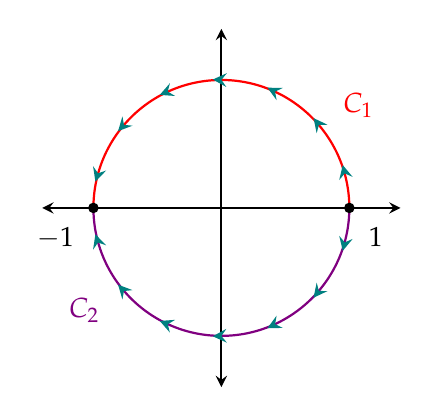
\begin{tikzpicture}[scale=1.3]
    \draw[<->,thick] (-1.75,0)--(1.75,0);
	\draw[<->,thick] (0,-1.75)--(0,1.75);
	\node[label=below left:{$-1$}](A) at (-1.25,0) {};
	\node[label=below right:{$1$}](B) at (1.25,0) {};
    \begin{scope}
        \node[label=right:{\color{red}$C_1$}](C) at (1,1) {};
        \draw[use Hobby shortcut,clockwise arrows,thick,red]
	(-1.25,0) .. (0,1.25) .. (1.25,0);
        \node[label=left:{\color{violet}$C_2$}](D) at (-1,-1) {};
        \draw[use Hobby shortcut,clockwise arrows,thick,violet]
	(-1.25,0) .. (0,-1.25) .. (1.25,0);
    \end{scope}
    \draw [fill=black] (A) circle (1.3pt);
    \draw [fill=black] (B) circle (1.3pt);
\end{tikzpicture}\]
But on the other hand we have also seen that
\[\int_C\,z\ dz = \frac{z_2^2 - z_1^2}{2}\]
for any contour $C$ with initial point $z_1$ and end point $z_2$.\\
\\
The difference between these functions turns out to be that $f(z) = z$ has an antiderivative on $\cc$ while $g(z) = 1/z$ does not any domain containing $C_1$ and $C_2$. 
\end{discussion}

\medskip

\begin{definition}[Antiderivative]
Suppose that $f$ is a continuous function on a domain $G$. Any holomorphic function $F:G \to \cc$ is called an \cdef{antiderivative} of $f$ if $F'(z) = f(z)$ for every $z \in G$. 
\end{definition}

\medskip

\begin{definition}[Independence of Path]
Let $f: G \to \cc$ be a continuous function on a domain $G$ and fix $z_1,\,z_2 \in G$. If
\[\int_{C_1}\,f(z)\ dz = \int_{C_2}\,f(z)\ dz\]
for any pair of contours $C_1$ and $C_2$ joining $z_1$ to $z_2$, then the integral of $f$ from $z_1$ to $z_2$ is \emph{independent of path} and we denote the unique value by
\[\int_{z_1}^{z_2}\,f(z)\ dz.\]
So, for instance, we would write
\[\int_{z_1}^{z_1}\,z\ dz = \frac{z_2^2 - z_1^2}{2},\]
since we have already proved the integral of $f(z) = z$ from $z_1$ to $z_2$, for any $z_1,\,z_2 \in \cc$, is independent of path. 
\end{definition} 

\medskip

\begin{theorem}[Fundamental Theorem of Contour Integrals]\label{FTCoCI}
Suppose $f$ is continuous on a domain $G$. The following are equivalent. 
\begin{itemize}
\item[(1)] $f$ has an antiderivative $F: G \to \cc$. 
\item[(2)] For all $z_1,\,z_2 \in G$, the integral of $f$ from $z_1$ to $z_2$ are independent of path.
\item[(3)] If $C$ is any closed contour lying in $G$, then
\[\int_C\,f(z)\ dz = 0\]
\end{itemize}
If any of these conditions hold, then the unique value of the integral in (2) is given as
\[\int_{z_1}^{z_2}\,f(z)\ dz = F(z_2) - F(z_1)\]
where $F$ is the antiderivative given in (1).
\end{theorem}
\begin{proof}\hfill
\begin{itemize}[leftmargin=4.5em,itemsep=1.5em]
\item[(1) $\Rightarrow$ (2)] Suppose $f$ has an antiderivative $F: G \to \cc$. Let $z_1,\,z_2 \in G$ and let $C$ be any contour with initial point $z_1$ to $z_2$ and lying in $G$.\\[0.5em]
First assume $C$ is a smooth arc parametrised by $z:[a,b] \to \cc$; therefore, in particular, $z(a) = z_1$ and $z(b) = z_2$. Then we first note
\[(F\circ z)'(t) = F'(z(t))z'(t) = f(z(t))z'(t)\]
That is, we have found an antiderivative of $f(z(t))z'(t)$, the function $F\circ z$. Hence, 
\begin{align*}
\int_C\,f(z)\ dz &= \int_a^b\,f(z(t))z'(t)\ dt\\[1em]
&= F(z(a)) - F(z(b)),\quad \text{by Proposition \ref{pathftc}}\\[0.5em]
&= F(z_2) - F(z_1)
\end{align*}
Now, assume $C$ is a contour; that is, we can write $C = C_1 + \cdots + C_n$, where $C_i$'s are smooth arcs with initial point $w_i$ and end point $w_{i + 1}$. In particular, $w_1 = z_1$ and $w_{n+1} = z_2$. Then,
\begin{align*}
\int_C\,f(z)\ dz &= \sum_{i=1}^n\int_{C_i}\,f(z)\ dz\\[1em]
 &= \sum_{i=1}^n F(w_{i+1}) - F(w_i)\\[0.5em]
 &= F(w_{n+1}) - F(w_1)\\[0.5em]
 &= F(z_2) - F(z_1)
\end{align*}
Since $F(z_2) - F(z_1)$ only depends on $z_1$ and $z_2$ and note the contour itself, we have proved the claim.

\item[(2) $\Rightarrow$ (3)] Let $C$ be any closed contour lying in $G$, and choose two distinct point $z_1$ and $z_2$ on $C$. Let $C_1$ and $C_2$ be contours from $z_1$ to $z_2$ such that $C = C_1 - C_2$.
\[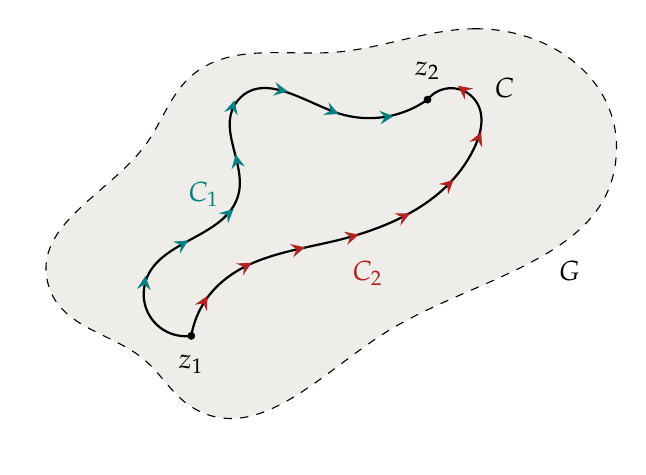
\begin{tikzpicture}[scale=0.6]
%    \draw[<->,thick] (-2,0)--(5,0);
%	\draw[<->,thick] (0,-2)--(0,5);
    \begin{scope}
    \draw[use Hobby shortcut,closed=true,fill=dirt,fill opacity=1/10,dashed]
	(5,5.5) .. (8,3) .. (3,-1) .. (-1,-2.5) .. (-2,-1.5) .. (-4,0) .. (-2,3) .. (-1,4.5) .. (2,5);
    \end{scope}
    \node[label=below:{$G$}](A) at (7,1) {};
\begin{scope}
        \node[label=left:{$C$}] at (6.25,4.25) {};
        \node[label=left:{\color{teal}$C_1$}](A) at (0,2) {};
        \node[label=below right:{\color{firebrick}$C_2$}](B) at (2,1) {};
        \node[label=above:{$z_2$}](C) at (4,4) {};
        \node[label=below:{$z_1$}](D) at (-1,-1) {};
        \draw[use Hobby shortcut,clockwise arrows,thick]
	(4,4) .. (2,3.75) .. (0,4) .. (0,2) .. (-2,0) .. (-1,-1);
        \draw[use Hobby shortcut,clockwise arrowsnew,thick]
	(4,4) .. (5,4) .. (5,3) .. (2,1) .. (-0.5,0) .. (-1,-1);
    \end{scope}
    \draw [fill=black] (C) circle (2pt);
    \draw [fill=black] (D) circle (2pt);
\end{tikzpicture}\]
By assumption, the integral of $f$ from $z_1$ to $z_2$ is independent of path, therefore
\[\int_{C_1}\,f(z)\ dz = \int_{C_2}\,f(z)\ dz\]
Hence,
\begin{align*}
\int_C\,f(z)\ dz &= \int_{C_1 - C_2}\,f(z)\ dz = \int_{C_1}\,f(z)\ dz - \int_{C_2}\,f(z)\ dz = 0,
\end{align*}
as claimed.

\item[(3) $\Rightarrow$ (2)] Suppose
\[\int_C\,f(z)\ dz = 0\]
for any closed contour $C$ lying in $G$. Let $z_1,\,z_2 \in G$ and $C_1$ and $C_2$ are two contour with initial point $z_1$ and end point $z_2$. Then $C_1  - C_2$ is a closed contour, and therefore by assumption
\begin{align*}
0 &= \int_{C_1 - C_2}\,f(z)\ dz = \int_{C_1}\,f(z)\ dz - \int_{C_2}\,f(z)\ dz
\end{align*}
Hence, 
\[\int_{C_1}\,f(z)\ dz = \int_{C_2}\,f(z)\ dz,\]
as claimed.

\item[(2) $\Rightarrow$ (1)] Assume (2) (and also (3), since we've shown them to be equivalent). We need to show that $f$ has an antiderivative on $G$. Fix any point $z_0 \in G$ and define
\[F(w) = \int_{z_0}^w\,f(z)\ dz,\]
which is well defined by (2). We need to show $F'(w) = f(w)$ for any $w \in G$. That is, 
\[\lim_{h \to 0}\frac{F(w + h) - F(w)}{h} = f(w)\]
Let $\epsilon > 0$ and consider an $z \in G$. Since $f$ is continuous at $z$, we can find $\delta > 0$ such that 
\[\text{if }\abs{z - w} < \delta,\quad \text{then }\abs{f(z) - f(w)} < \epsilon\]
For $w \in G$, since $G$ is a domain and so in particular an open set, we can find a $d>0$ such that $D_d(w) \subseteq G$. Pick a $h \in \cc$ such that $0< \abs{h} < \min\set{d,\delta}$. Then $0 < \abs{h} < d$ and $0 < \abs{h} < \delta$. In particular, $w + h \in D_d(w) \subseteq G$; then,
\begin{align*}
F(w + h) - F(w) &= \int_{z_0}^{w+h}\,f(z)\ dz - \int_{z_0}^w\,f(z)\ dz = \int_{w}^{w+h}\,f(z)\ dz
\end{align*}
Since our integrals are path-independent, we assume that the integral above is over a line segment from $w$ to $w + h$, which lies in $G$, since $D_d(w)$ is convex. Also, 
\begin{align*}
f(w) &= \frac{f(w)h}{h} = \frac{1}{h}\,f(w)\,\int_{w}^{w+h}\,dz = \frac{1}{h}\,\int_{w}^{w+h}\,f(w)\ dz
\end{align*}
Also, since $\abs{h} < \delta$, then $\abs{z - w} < \delta$ for any point $z$ lying on $\ell$, the line segment joining $w$ to $w + h$. Therefore, $\abs{f(z) - f(w)} < \epsilon$ for any $z \in \ell$, that is, $\max_{z \in \ell}\abs{f(z) - f(w)} < \epsilon$.\\[0.5em]
\[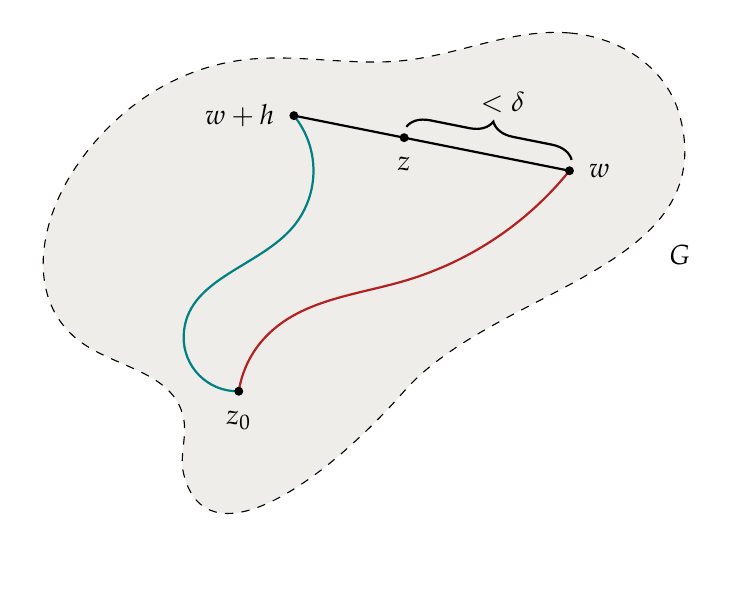
\begin{tikzpicture}[scale=0.7]
%    \draw[<->,thick] (-2,0)--(5,0);
%	\draw[<->,thick] (0,-2)--(0,5);
    \begin{scope}
    \draw[use Hobby shortcut,closed=true,fill=dirt,fill opacity=1/10,dashed]
	(5,5.5) .. (7,4) .. (2,-1) .. (-2,-2.5) .. (-2,-1.5) .. (-4,0) .. (-4,3) .. (-1,5) .. (2,5);
    \end{scope}
    \node[label=below:{$G$}](A) at (7,2) {};
\begin{scope}
%        \node[label=left:{$C$}] at (6.25,4.25) {};
%        \node[label=left:{\color{teal}$C_1$}](A) at (0,2) {};
%        \node[label=below right:{\color{firebrick}$C_2$}](B) at (2,1) {};
        \node[label=right:{$w$}](C) at (5,3) {};
        \node[label=left:{$w + h$}](D) at (0,4) {};
        \node[label=below:{$z_0$}](E) at (-1,-1) {};
        \node[label=below:{$z$}](F) at (2,3.6) {};
        \draw[use Hobby shortcut,thick,teal]
	(0,4) .. (0,2) .. (-2,0) .. (-1,-1);
        \draw[use Hobby shortcut,thick,firebrick]
	(5,3) .. (2,1) .. (-0.5,0) .. (-1,-1);
    \end{scope}
    \draw[thick] (0,4)--(5,3);
    \draw [fill=black] (C) circle (2pt);
    \draw [fill=black] (D) circle (2pt);
    \draw [fill=black] (E) circle (2pt);
    \draw [fill=black] (F) circle (2pt);
    \draw [decorate,decoration={brace,amplitude=8pt,mirror,raise=4pt},yshift=0pt,thick]
(5,3) -- (2,3.6) node [black,midway,above,xshift=0.2cm,yshift=0.4cm] {$\footnotesize <\delta$};
\end{tikzpicture}\]
Using the preceding computations we have
\begin{align*}
\abs{\frac{F(w + h) - F(w)}{h} - f(w)} &= \abs{\frac{1}{h}\,\int_{w}^{w+h}\,f(z)\ dz - \frac{1}{h}\,\int_{w}^{w+h}\,f(w)\ dz}\\[1em]
 &= \frac{1}{h}\,\abs{\int_{w}^{w+h}\,f(z) - f(w)\ dz}\\[1em]
 &\leq \frac{1}{h}\,\max_{z \in \ell}\abs{f(z) - f(w)}\cdot L(\ell)\\[1em]
 &< \frac{\epsilon}{h}\cdot L(\ell)\\[1em]
 &= \epsilon,\quad \text{since $L(\ell) = h$}
\end{align*}
We have shown that given an $\epsilon > 0$, there exists a $\delta > 0$ such that
\[\text{if }\abs{h} < \delta,\quad \text{then }\abs{\frac{F(w + h) - F(w)}{h} - f(w)} < \epsilon\]
That is, $F'(w) = f(w)$, for all $w \in G$.
\end{itemize}
\vspace*{-\baselineskip}
\end{proof}

\medskip

\begin{example}\lecmargin{24}\hfill
\begin{itemize}
\item[(1)] The function $f(z) = 1/z$ has no antiderivative on $\cc^*$. In fact, it has no antiderivative on any domain $G$ containing a deleted neighbourhood of $0$. Take a circle $C_\epsilon = C_\epsilon(0)$ with radius $\epsilon > 0$ such that it lies in our domain $G$.
\[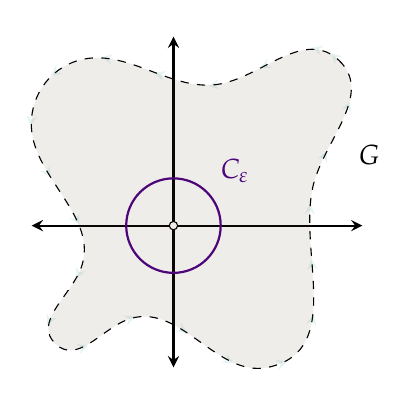
\begin{tikzpicture}[scale=0.6]
    \draw[<->,thick] (-2,1)--(5,1);
	\draw[<->,thick] (1,-2)--(1,5);
    \draw [fill=white] (1,1) circle (2.5pt);
	\draw[indigo,thick](1,1) circle (1);
    \node[label={\color{indigo}$C_\epsilon$}] at (2.3,1.5) {};
    \node[label=right:{$G$}] at (4.5,2.5) {};
	\begin{scope}
    \draw[use Hobby shortcut,closed=true,wise arrows,fill=dirt,fill opacity=1/10,dashed]
	(4.5,4.5) .. (4,2) .. (3,-2) .. (0,-1) .. (-1.5,-1.5) .. (-1,0) .. (-2,3) .. (-1,4.5) .. (2,4) .. (4.5,4.5);
    \end{scope}
\end{tikzpicture}\]
Then,
\begin{align*}
\int_{C_\epsilon}\,\frac{1}{z}\ dz &= \int_{0}^{2\pi}\,\frac{1}{\epsilon e^{it}}\,i\epsilon e^{it}\ dt\\[1em]
 &= \int_{0}^{2\pi}\,i\ dt\\[1em]
 &= 2\pi i
\end{align*}
By Theorem \ref{FTCoCI}, $f(z)$ does not have an antiderivative on such a domain, as the integral over the closed contour $C_\epsilon$ was non-zero. The problem is as follows: it is true that that a branch of the logarithm $F(z) = \log z$ is such that 
\[F'(z) = \frac{1}{z},\]
but it is only holomorphic on the complement of the branch cut. Since our domain contains a deleted neighbourhood of $0$, it has a non-empty intersection with any branch cut we take, and therefore $F$ is not holomorphic on $G$. This argument, in particular, holds for the domain $\cc^*$.

\item[(2)] The function $f(z) = \cos z$ is entire on $\cc$, so is $F(z) = \sin z$. Moreover $F'(z) = \cos z = f(z)$, so $f$ has an antiderivative on $\cc$. So, for instance
\begin{align*}
\int_0^{\pi i}\,\cos z\ dz &= \sin\pi i - \sin 0 = \sin\pi i
\end{align*}

\item[(3)] Although $f(z) = 1/z$ has no antiderivative on any domain containing a deleted neighbourhood of $0$, we can integrate $f$ over a circle $C$ by using two different antiderivatives.\\
\\
Let $C_1$ be parametrised by $z(t) = e^{it},\, t \in [-\pi/2,\pi/2]$, a contour from $-i$ to $i$.
\[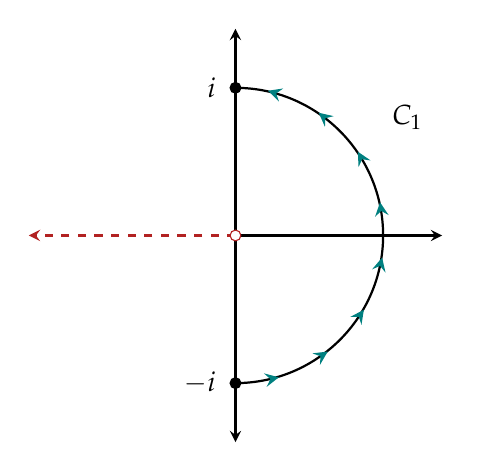
\begin{tikzpicture}[scale=1.5]
    \draw[<-,thick] (1.75,0)--(0,0);
	\draw[<->,thick] (0,-1.75)--(0,1.75);
    \begin{scope}
        \node[label=left:{$C_1$}](A) at (1.75,1) {};
        \node[label=left:{$-i$}](B) at (0,-1.25) {};
        \node[label=left:{$i$}](C) at (0,1.25) {};
        \draw[use Hobby shortcut,clockwise arrows,thick]
	(0,1.25) .. (1.25,0) .. (0,-1.25);
    \end{scope}
	\draw[->,thick,dashed,firebrick] (0,0)--(-1.75,0);
    \draw [firebrick,fill=white] (0,0) circle (1.3pt);
    \draw [fill=black] (B) circle (1.3pt);
    \draw [fill=black] (C) circle (1.3pt);
\end{tikzpicture}\]
On $\cc\setminus \rr_{\leq 0}$, $f(z)$ has an antiderivative, namely the principal branch of the logarithm
\[\plog z = \ln\abs{z} + i\parg z,\quad -\pi < \parg z < \pi\]
Then, by Theorem \ref{FTCoCI}
\begin{align*}
\int_{C_1}\,\frac{1}{z}\ dz &= \plog i - \plog(-i)\\[0.5em]
&= \left(\ln\abs{i} + i\parg i\right) - \left(\ln\abs{-i} + i\parg (-i)\right)\\[0.5em]
&= \left(\ln 1 + i\frac{\pi}{2}\right) - \left(\ln 1 - i\frac{\pi}{2}\right)\\[0.5em]
&= \pi i
\end{align*}

\medskip

Let $C_2$ be parametrised by $z(t) = e^{it},\, t \in [\pi/2,3\pi/2]$, a contour from $i$ to $-i$.
\[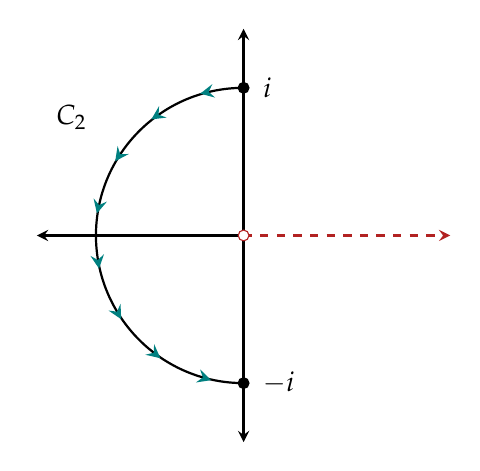
\begin{tikzpicture}[scale=1.5]
    \draw[<-,thick] (-1.75,0)--(0,0);
	\draw[<->,thick] (0,-1.75)--(0,1.75);
    \begin{scope}
        \node[label=right:{$C_2$}](A) at (-1.75,1) {};
        \node[label=right:{$-i$}](B) at (0,-1.25) {};
        \node[label=right:{$i$}](C) at (0,1.25) {};
        \draw[use Hobby shortcut,clockwise arrows,thick]
	(0,-1.25) .. (-1.25,0) .. (0,1.25);
    \end{scope}
	\draw[->,thick,dashed,firebrick] (0,0)--(1.75,0);
    \draw [firebrick,fill=white] (0,0) circle (1.3pt);
    \draw [fill=black] (B) circle (1.3pt);
    \draw [fill=black] (C) circle (1.3pt);
\end{tikzpicture}\]
On $\cc\setminus \rr_{\geq 0}$, $f(z)$ has an antiderivative, namely the following branch of the logarithm
\[\log z = \ln\abs{z} + i\arg z,\quad 0 < \arg z < 2\pi\]
Then, by Theorem \ref{FTCoCI}
\begin{align*}
\int_{C_2}\,\frac{1}{z}\ dz &= \log (-i) - \log i\\[0.5em]
&= \left(\ln\abs{i} + i\arg (-i)\right) - \left(\ln\abs{-i} + i\arg i\right)\\[0.5em]
&= \left(\ln 1 + i\frac{3\pi}{2}\right) - \left(\ln 1 + i\frac{\pi}{2}\right)\\[0.5em]
&= \pi i
\end{align*}
Hence, 
\[\int_C\,\frac{1}{z}\ dz = \int_{C_1}\,\frac{1}{z}\ dz + \int_{C_2}\,\frac{1}{z}\ dz = \pi i + \pi i = 2\pi i\]
\end{itemize}
\end{example}

\bigskip

\subsection{Cauchy-Goursat Theorem}
%\begin{mdframed}
%\begin{center}
%{\Large Cauchy-Goursat Theorem}
%\end{center}
%\end{mdframed}

\begin{discussion}
The Cauchy-Goursat theorem gives a sufficient condition for the integral of a function over a simple closed curve to be zero. The theorem has powerful implications, ultimately it leads to
\begin{itemize}
\item The Cauchy Integral formula.
\item The theory of residues for computing contour integrals.
\item A method to evaluate real-valued functions in a real variable, using contour integration.
\end{itemize}
Historically, a weaker version of the theorem was first proved by Cauchy. We prove this first.\\
\\
We first note the following.
\begin{itemize}
\item[(1)] Contour integrals are related to line (or path) integrals. We note this by writing our function $f(z) = f(x + iy) = u(x,y) + i\,v(x,y)$ and formally writing $dz = dx + i\,dy$. Then formally,
\begin{align*}
\int_C\,f(z)\ dz &= \int_C\, (u + iv)(dx + idy)\\[1em]
&= \int_C\, u\,dx - v\,dy + i\int_C\,u\,dy + v\,dx
\end{align*}

\item[(2)] \textbf{Green's Theorem.} Suppose $C$ is a simple closed contour in $\rr^2$ and let $R$ be the region enclosed by $C$ and including $C$. If $P(x,y)$ and $Q(x,y)$ have continuous partial derivatives on $R$. Then
\[\int_C\,P\,dx + Q\,dy = \iint_R\,\frac{\partial Q}{\partial x} - \frac{\partial P}{\partial y}\ dA = \iint_R\,(Q_x - P_y)\ dA\]
\end{itemize}
\end{discussion}

\medskip

\begin{theorem}[Weak Cauchy Integral Theorem]
Let $C$ be a simple closed contour, and let $R$ denote the region consisting of $C$ and its interior. If $f$ is holomorphic on $R$ and $f'$ continuous on $R$, then
\[\int_C\,f(z)\ dz = 0.\]
\end{theorem}
\begin{proof}
If $f(z) = u(x,y) + i\,v(x,y)$ is holomorphic on $R$, then the Cauchy-Riemann equations hold, and so $u_x = v_y$ and $u_y = -v_x$ on $R$, and $f'(z) = u_x + i\,v_x = v_y - i\,u_y$.\\[0.5em]
Since $f'$ is continuous, so are $u_x,\,u_y,\,v_x$ and $v_y$. Hence, 
\begin{align*}
\int_C\,f(z)\ dz &= \int_C\, u\,dx - v\,dy + i\int_C\,u\,dy + v\,dx\\[1em]
 &= \iint_R (-v_x-u_y)\ dA + i\iint_R (u_x - v_y)\ dA,\quad \text{by Green's theorem}\\[1em]
 &= 0,\quad \text{using Cauchy-Riemann equations}\\[-3em]
\end{align*}
\end{proof}

\medskip

Goursat was the first to prove that the assumption on the continuity of $f'$ can be omitted. This turns out to be essential for the theory of holomorphic functions. The problem is that it may be difficult to prove the derivative of holomorphic function is continuous. 

\begin{theorem}[Cauchy-Goursat Theorem]\label{cgthm}
Let $C$ be a simple closed contour, and let $R$ denote the region consisting of $C$ and its interior. If $f$ is holomorphic on $R$, then
\[\int_C\,f(z)\ dz = 0.\]
\end{theorem}
\begin{proof}[Proof (skipped in class)]
\textbf{For simplicity, we will assume $\mathbold{C}$ is a square.} The idea is to ``divide and conquer". We break the curve into a finite number of smaller squares on which we can estimate the integral. We first construct a sequence of positively oriented curves $S^{(k)}$, each of which is the boundary of a square region $R^{(k)}$.\\
\\
To begin with, set $S^{(0)} = C$. Then, inductively, after the first $k$ squares have been chosen, we define $(k+1)^{\text{th}}$ square as follows. Divide $S^{(k)}$ into four congruent squares with positive orientation: $S^{(k)}_1,\,S^{(k)}_2,\,S^{(k)}_3,\,S^{(k)}_4$.
\[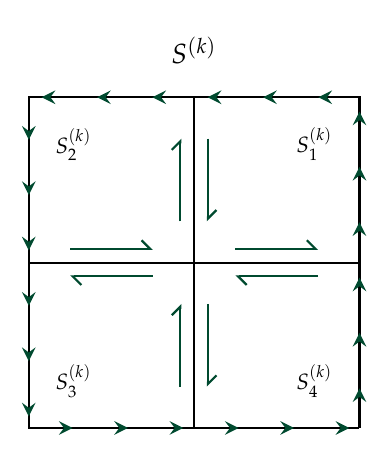
\begin{tikzpicture}[scale=0.7]
    \begin{scope}
    \draw[clockwise arrowsnewsquare,thick]
	(3,-3) -- (3,3) -- (-3,3) -- (-3,-3) -- (3,-3);
	\draw[thick]
	(0,-3) -- (0,3);
	\draw[thick]
	(-3,0) -- (3,0);
	\draw[-{Straight Barb[left]},forest,thick]
	(-2.25,0.25) -- (-0.75,0.25);	
	\draw[-{Straight Barb[left]},forest,thick]
	(0.75,0.25) -- (2.25,0.25);	
	\draw[-{Straight Barb[left]},forest,thick]
	(-0.75,-0.25) -- (-2.25,-0.25);	
	\draw[-{Straight Barb[left]},forest,thick]
	(2.25,-0.25) -- (0.75,-0.25);	
	\draw[-{Straight Barb[left]},forest,thick]
	(0.25,2.25) -- (0.25,0.75);	
	\draw[-{Straight Barb[left]},forest,thick]
	(-0.25,0.75) -- (-0.25,2.25);	
	\draw[-{Straight Barb[left]},forest,thick]
	(0.25,-0.75) -- (0.25,-2.25);	
	\draw[-{Straight Barb[left]},forest,thick]
	(-0.25,-2.25) -- (-0.25,-0.75);	
    \end{scope}
    \node[label=above:{$S^{(k)}$}] at (0,3.25) {};
    \node[label=below right:{\footnotesize$S_4^{(k)}$}](A) at (1.5,-1.5) {};
    \node[label=below left:{\footnotesize$S_3^{(k)}$}](A) at (-1.5,-1.5) {};
    \node[label=above right:{\footnotesize$S_1^{(k)}$}](A) at (1.5,1.5) {};
    \node[label=above left:{\footnotesize$S_2^{(k)}$}](A) at (-1.5,1.5) {};
\end{tikzpicture}\]\\
Note that the integral of $f$ along the shared boundaries of these squares cancel. Hence, 
\[\sum_{i=1}^4\int_{S^{(k)}_i}f(z)\ dz = \int_{S^{(k)}}f(z)\ dz\]
We choose $S^{(k+1)}$ to be one of the squares $S^{(k)}_j$ such that 
\[\abs{\int_{S^{(k+1)}}f(z)\ dz} = \abs{\int_{S^{(k)}_j}f(z)\ dz} = \abs{\max_{i=1}^4\int_{S^{(k)}_i}f(z)\ dz}\]
At this point, we have a sequence $S^{(0)},\ldots,S^{(k)},\ldots$. Note that, by triangle inequality
\begin{align*}
\abs{\int_{S^{(k)}}f(z)\ dz} & \leq \sum_{i=1}^4\abs{\int_{S^{(k)}_i}f(z)\ dz} \leq 4\abs{\int_{S^{(k+1)}}f(z)\ dz}
\end{align*}
So, inductively we get
\[\abs{\int_{C}\,f(z)\ dz} = \abs{\int_{S^{(0)}}f(z)\ dz} \leq 4^n\abs{\int_{S^{(n)}}f(z)\ dz} \tag{$*$}\]
We record some more facts. Denote by $d^{(n)}$ the length of the diagonal of the $n^{\text{th}}$ square $S^{(n)}$ and denote by $P^{(n)}$ its perimeter. Then,
\begin{align*}
d^{(n)} &= \frac{1}{2^n}\cdot d^{(0)}\\[0.5em]
p^{(n)} &= \frac{1}{2^n}\cdot p^{(0)}
\end{align*}
Also, $d^{(n)},\,p^{(n)} \to 0$, as $n \to \infty$.\\
\\
Next, consider the associated sequence of regions
\[R = R^{(0)} \supseteq R^{(1)} \supseteq \cdots \supseteq R^{(k)} \supseteq \cdots.\]
Each $R^{(k)}$ is compact (closed and bounded) and hence, using a fact from topology, there exists a unique point
\[z_0 \in \bigcap_{i\geq 0}R^{(i)}.\]
Since $z_0 \in R^{(0)} = R$, $f$ is holomorphic at $z_0$. So, we define the following function on $R$
\[\psi(z) = \begin{cases} \dfrac{f(z) - f(z_0)}{z - z_0} - f'(z_0) & \text{if $z \neq z_0$}\\[1em] 0 & \text{if $z = z_0$} \end{cases}\]
and we note
\[\lim_{z \to z_0}\psi(z) = f'(z_0) - f'(z_0) = 0 = \psi(z_0),\]
and therefore $\psi$ is continuous at $z_0$. We can write
\[f(z) = f(z_0) + (z-z_0)(\psi(z) + f'(z_0)) = f(z_0) + f'(z_0)(z - z_0) + \psi(z)(z - z_0)\]
Note that $f(z_0)$ and $f'(z_0)(z - z_0)$ have antiderivatives on $\cc$, hence, by Theorem \ref{FTCoCI}, we have
\begin{align*}
\int_{S^{(n)}}f(z)\ dz &= \int_{S^{(n)}}f(z_0)\ dz + \int_{S^{(n)}}f'(z_0)(z - z_0)\ dz + \int_{S^{(n)}}\psi(z)(z - z_0)\ dz\\[1em]
&= 0 + 0 + \int_{S^{(n)}}\psi(z)(z - z_0)\ dz\\[1em]
&= \int_{S^{(n)}}\psi(z)(z - z_0)\ dz
\end{align*}
Consider $\epsilon > 0$. Since $\psi$ is continuous at $z_0$ with $\psi(z_0) = 0$, choose $\delta > 0$ such that
\[\text{if } \abs{z - z_0} < \delta,\quad \text{then } \abs{\psi(z)} < \epsilon\]
Since $d^{(n)} \to 0$, as $n \to \infty$, we choose an $N \in \zz_{>0}$ such that $|d^{(n)}|< \delta$ for every $n \geq N$. Thus, if $z \in S^{(N)}$, then $\abs{z - z_0} < |d^{(N)}| < \delta$ and therefore $\abs{\psi(z)} < \epsilon$ for every $z \in S^{(N)}$. Hence, 
\[\max_{z \in S^{(N)}} \abs{z - z_0} < d^{(N)} \quad \text{and} \quad \max_{z \in S^{(N)}} \abs{\psi(z)} < \epsilon\]
Hence, we obtain
\begin{align*}
\abs{\int_{S^{(N)}}f(z)\ dz} &= \abs{\int_{S^{(N)}}\psi(z)(z - z_0)\ dz}\\[1em]
 &\leq \max_{z \in S^{(N)}}\abs{\psi(z)}\abs{z - z_0}\cdot L(S^{(N)})\\[0.5em]
 &< \epsilon\cdot d^{(N)}\cdot L(S^{(N)})\\[0.5em]
 &= d^{(N)}p^{(N)}\epsilon\\[0.5em]
 &= \frac{1}{4^N}\,d^{(0)}p^{(0)}\epsilon
\end{align*}
By ($*$), we have
\begin{align*}
\abs{\int_C\,f(z)\ dz} &\leq 4^N\abs{\int_{S^{(N)}}f(z)\ dz}\\[1em]
 &< 4^N\cdot \frac{1}{4^N}\,d^{(0)}p^{(0)}\epsilon\\[1em]
 &= d^{(0)}p^{(0)}\epsilon
\end{align*}
Since $\epsilon > 0$ is arbitrary, we necessarily get that
\[\abs{\int_C\,f(z)\ dz} \leq 0\]
Thus, 
\[\int_C\,f(z)\ dz = 0\]
\end{proof}

\bigskip

\subsection{Simply Connected Domains}
%\begin{mdframed}
%\begin{center}
%{\Large Simply Connected Domains}
%\end{center}
%\end{mdframed}

\begin{definition}[Simply Connected Domain]
A domain $G$ is called \cdef{simply\ connected} if it has the following property: if $C$ is any simple closed contour lying in $G$ and $z$ is interior to $C$, then $z \in G$.\\[0.5em]
Intuitively, a simply connected domain is a domain that has no ``holes".\\
\\
Open disks, complex plane, interior of any simple closed contour etc. are all examples of simply connected domains. While deleted open disks, $\cc\setminus\set{p}$ etc. are examples of non-simply connected domains.
\end{definition}

\medskip

A result similar to Theorem \ref{cgthm} holds for closed contours, not necessarily simple, provided they lie in a simply connected domain.
\begin{theorem}[Cauchy-Goursat Theorem for Simply Connected Domain]\label{cgthmsc}
Suppose $f$ is holomorphic on a simply connected $G$. If $C$ is any closed contour lying in $G$, then
\[\int_C\, f(z)\ dz = 0.\]
\end{theorem}
\begin{proof}
We are presented with two cases: $C$ has finitely many self-intersections, or infinitely many self-intersections. Let's focus on the first cases, where the proof is a consequence of Theorem \ref{cgthm}.
\[\begin{tikzpicture}[scale=1.2]
    \begin{scope}
    \draw[use Hobby shortcut,closed=true,fill=dirt,fill opacity=1/10,dashed]
	(7.75,0) .. (5,-1.5) .. (3,-1) .. (1,-1.5) .. (-1,-1.25) .. (-1.5,-1.5) .. (-3.75,0) .. (-1.5,1) .. (-1,1) .. (1,1.5) .. (3,1) .. (5,1.5) .. (7.75,0);
    \end{scope}
    \node[label=below:{$G$}] at (3,-1.25) {};
\begin{scope}
        \node[label=above:{$C$}] at (1.75,0.5) {};
        \node[label=below:{\color{teal}$C_1$}](A) at (-2,-0.5) {};
        \node[label=below:{\color{firebrick}$C_2$}](B) at (0,-0.5) {};
        \node[label=below:{\color{indigo}$C_{n+1}$}](B) at (6,-0.5) {};
        \draw[use Hobby shortcut,clockwise arrows,thick]
	(-1,0) .. (-2,-0.5) .. (-3,0) .. (-2,0.5) .. (-1,0);
        \draw[use Hobby shortcut,clockwise arrowsnew,thick]
	(-1,0) .. (0,0.5) .. (1.5,0);
        \draw[use Hobby shortcut,clockwise arrowsnew,thick]
	(1.5,0) .. (0,-0.5) .. (-1,0);
        \draw[use Hobby shortcut,thick]
	(2.5,0.5) .. (2,0.35) .. (1.5,0);
        \draw[use Hobby shortcut,thick]
	(1.5,0) .. (2,-0.35) .. (2.5,-0.5);
        \draw[use Hobby shortcut,thick]
	(5,0) .. (4.5,0.325) .. (4,0.5);
        \draw[use Hobby shortcut,thick]
	(4,-0.5) .. (4.5,-0.325) .. (5,0);
        \draw[use Hobby shortcut,clockwise arrowsmult,thick]
	(5,0) .. (6,-0.5) .. (7,0) .. (6,0.5) .. (5,0);
	\draw[loosely dotted,thick]
	(2.75,0.5)  -- (3.75,0.5);
	\draw[loosely dotted,thick]
	(2.75,-0.5)  -- (3.75,-0.5);
    \end{scope}
\end{tikzpicture}\]
Suppose $C$ has $n$-many self-intersections, then those points of self-intersections allow us to write \[C = C_1 + C_2 + \cdots + C_{n+1},\] where each $C_i$ is a simple closed contour that all, necessarily, lie in $G$.\\
\\
Therefore $f$ is holomorphic at each point interior of and on $C_i$, hence by Theorem \ref{cgthm} we get
\[\int_{C_i}\,f(z)\ dz = 0\]
Finally, we have\\
\[\int_C\,f(z)\ dz = \sum_{i=1}^n\int_{C_i}\,f(z)\ dz = 0\]
as claimed.\\
\\
The proof in the case the contour has infinitely many self-intersections is subtle , so we assume validity without a proof. 
\end{proof}

\medskip

\begin{corollary}[Antiderivatives of Holomorphic Functions]\label{holantisc}
If $f$ is holomorphic on a simply connected domain $G$, then $f$ has an antiderivative on $G$.
\end{corollary}
\begin{proof}
By Theorem \ref{cgthmsc}, 
\[\int_C\,f(z)\ dz = 0\]
for any closed contour $C$ lying in $G$. By Theorem \ref{FTCoCI}, this is equivalent to $f$ having an antiderivative on $G$.
\end{proof}

\medskip

\begin{corollary}[Entire Functions have Antiderivatives]
Suppose $f$ is entire, then $f$ has an antiderivative on $\cc$ which is necessarily also entire.
\end{corollary}
\begin{proof}
$\cc$ is simply connected, the result follows from Corollary \ref{holantisc}.
\end{proof}

\bigskip

\subsection{Multiply Connected Domains}
%\begin{mdframed}
%\begin{center}
%{\Large Multiply Connected Domains}
%\end{center}
%\end{mdframed}

\begin{definition}[Multiply Connected Domain]
A domain $G$ is called \cdef{multiply\ connected} if it not simply connected.
\end{definition}

\medskip

We can generalise Theorem \ref{cgthmsc} to a multiply connected domain with finitely many holes.
\begin{theorem}[Generalised Cauchy-Goursat Theorem]\label{cgthmgen}
\lecmargin{25}
Suppose that
\begin{itemize}
\item[(1)] $C$ is a simple closed positively oriented contour.
\item[(2)] $C_1,\ldots,C_n$ are simple closed negatively oriented contours enclosing regions $R_1,\ldots,R_n$. Further assume that the regions are pairwise disjoint and interior to $C$.
\end{itemize}
If $f$ is holomorphic on each contour and the region consisting of all points interior to $C$ but exterior to each $C_i$, then
\[\int_C\,f(z)\ dz + \sum_{i=1}^n\int_{C_i}f(z)\ dz = 0\]\\
\[\begin{tikzpicture}[scale=1]
    \begin{scope}
    \draw[use Hobby shortcut,closed=true,fill=forest,fill opacity=1/10,draw opacity=0]
	(10,0) .. (6,-1.5) .. (3,-1.25) .. (1,-1.5) .. (-1,-1.25) .. (-1.5,-1.5) .. (-3.75,-0.5) .. (-3.5,-0.5) .. (-3.75,0.5) .. (-1.5,1) .. (-1,1) .. (1,1.5) .. (3,1.25) .. (6,1.5) .. (10,0);
    \draw[use Hobby shortcut,closed=true,clockwise arrowsnewbound,thick]
	(10,0) .. (6,-1.5) .. (3,-1.25) .. (1,-1.5) .. (-1,-1.25) .. (-1.5,-1.5) .. (-3.75,-0.5) .. (-3.5,-0.5) .. (-3.75,0.5) .. (-1.5,1) .. (-1,1) .. (1,1.5) .. (3,1.25) .. (6,1.5) .. (10,0);
    \end{scope}
    \node[label=above:{$C$}] at (3,1.25) {};
\begin{scope}
        \node[label=below left:{$C_1$}](A) at (-2,-0.85) {};
        \node[label=below:{$C_2$}](B) at (1,-0.5) {};
        \node[label=below:{$C_{n-1}$}](C) at (5,-0.45) {};
        \node[label=below:{$C_n$}](D) at (8,-0.65) {};
        \draw[use Hobby shortcut,closed=true,clockwise arrowsmulthole,fill=white,thick]
	(4,0) .. (5,1) .. (6,0) .. (5,-0.5) .. (4,0);
        \draw[use Hobby shortcut,closed=true,clockwise arrowsmulthole,fill=white,thick]
	(-0.5,0) .. (0,0.75) .. (0.5,0.5) .. (1,0.5) .. (2,0) .. (1,-0.5) .. (0.5,-0.5) .. (0,-0.75) .. (-0.5,0);
		\draw[use Hobby shortcut,closed=true,clockwise arrowsmulthole,fill=white,thick]
	(-2.75,-0.25) .. (-2,0.5) .. (-1.25,-0.25) .. (-2,-1) .. (-2.75,-0.25);
        \draw[use Hobby shortcut,closed=true,clockwise arrowsmulthole,fill=white,thick]
	(7,-0.05) .. (8.5,0.95) .. (9,-0.05) .. (8.5,-0.55) .. (7,-0.05);
	\draw[loosely dotted,very thick]
	(2.5,0)  -- (3.5,0);
	\end{scope}
\end{tikzpicture}\qquad\quad\]\\[-4.5em]
\end{theorem}
\begin{proof}
We prove this using induction.\\
\\
\emph{Base Case. $n=1$.} Assume $C$ and $C_1$ are contour satisfying the hypotheses. Let $z_1,\,z_2$ be points on $C$ while $w_1,\,w_2$ be points on $C_1$. Join $z_1$ to $w_1$ with a polygon line $L_1$, and also join $z_2$ to $w_2$ with a polygon line $L_2$.\\
\\
Define contour $\Gamma_1$ and $\Gamma_2$ as follows.
\begin{itemize}
\item[$\Gamma_1$:] Start with $z_1$ and follow to $w_1$ along $L_1$, then $w_1$ to $w_2$ along $C_1$ (we'll call this $C_{11}$), then $w_2$ to $z_2$ along $L_2$, and finally $z_2$ to $z_1$ along $C$ (we'll call this $C'$). So, 
\[\Gamma_1 = L_1 + C_{11} + L_2 + C'\]
\item[$\Gamma_2$:] Start with $z_2$ and follow to $w_2$ along $-L_2$, then $w_2$ to $w_1$ along $C_1$ (we'll call this $C_{12}$), then $w_1$ to $z_1$ along $-L_1$, and finally $z_1$ to $z_2$ along $C$ (we'll call this $C''$). So, 
\[\Gamma_2 = -L_2 + C_{12} - L_1 + C''\]
\end{itemize}
\begin{center}
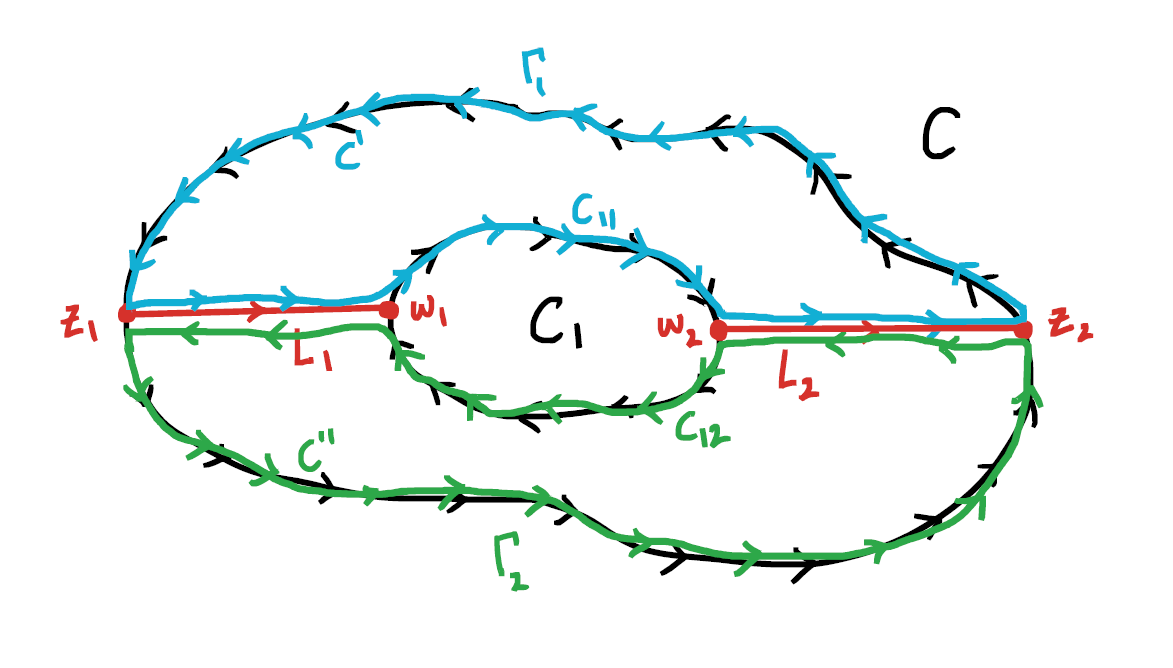
\includegraphics[scale=0.4]{Sections/Illustrations/CG-MCD-Base.png}
\end{center}
We note $C' + C'' = C$ and $C_{11} + C_{12} = C$.\\
\\
Then $f$ is holomorphic in the interior of and on the simple closed curves $\Gamma_1$ and $\Gamma_2$, so by Theorem \ref{cgthm} we have
\[\int_{\Gamma_1}f(z)\ dz = \int_{\Gamma_2}f(z)\ dz = 0\]
So, this gives us
\begin{align*}
0 &= \int_{\Gamma_1}f(z)\ dz + \int_{\Gamma_2}f(z)\ dz\\[1em]
 &= \left(\int_{L_1}f(z)\ dz + \int_{C_{11}}f(z)\ dz + \int_{L_2}f(z)\ dz + \int_{C'}f(z)\ dz\right)\\[1em]
 &\qquad + \left(-\int_{L_2}f(z)\ dz + \int_{C_{12}}f(z)\ dz - \int_{L_1}f(z)\ dz + \int_{C''}f(z)\ dz\right)\\[1em]
 &= \int_{C'}f(z)\ dz + \int_{C''}f(z)\ dz + \int_{C_{11}}f(z)\ dz + \int_{C_{12}}f(z)\ dz\\[1em]
 &= \int_{C}f(z)\ dz + \int_{C_1}f(z)\ dz
\end{align*}
\emph{Inductive Step.} Assume the statement holds for $n = k$, that is
\[\int_C\,f(z)\ dz + \sum_{i=1}^k\int_{C_i}f(z)\ dz = 0\]
for any $k$-many contours satisfying the hypotheses.\\
\\
Now, let $C_1,\ldots,C_k,C_{k+1}$ be any $k+1$-many contours. Introduce a polygon line $L$ that separates $C_1,\ldots,C_k$ from $C_{k+1}$, say with end points $z_1$ and $z_2$. We define $\Gamma_1$ and $\Gamma_2$ as follows.
\begin{itemize}
\item[$\Gamma_1$:] Start with $z_1$ and follow to $z_2$ along $C$ (we'll call this $C'$), then $z_2$ to $z_1$ along $-L$. So, 
\[\Gamma_1 = C' - L\]
\item[$\Gamma_2$:] Start with $z_1$ and follow to $z_2$ along $L$, then $z_2$ to $z_1$ along $C$ (we'll call this $C''$). So, 
\[\Gamma_2 = C'' + L\]
\end{itemize}
We note $C' + C'' = C$.
\begin{center}
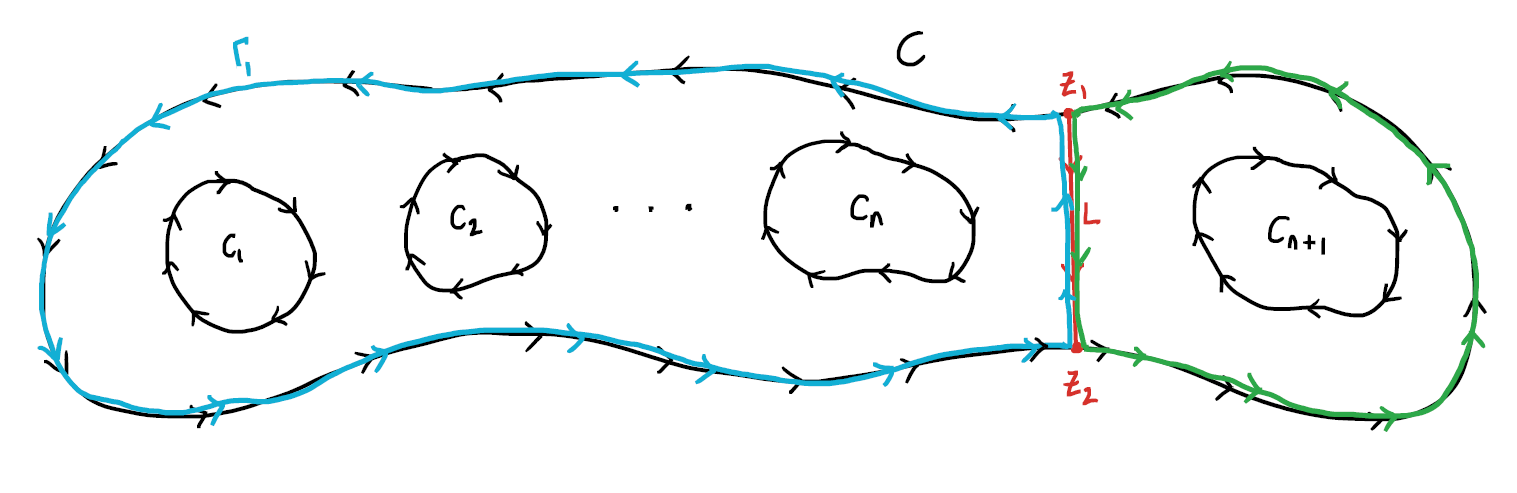
\includegraphics[scale=0.5]{Sections/Illustrations/CG-MCD-Induction.png}
\end{center}
We note that
\begin{align*}
\int_{\Gamma_1}f(z)\ dz + \int_{\Gamma_2}f(z)\ dz &= \left(\int_{C'}f(z)\ dz - \int_{L}\,f(z)\ dz\right) + \left(\int_{C''}f(z)\ dz + \int_{L}\,f(z)\ dz\right)\\[1em]
 &= \int_{C'}f(z)\ dz + \int_{C''}f(z)\ dz\\[1em]
 &= \int_C\,f(z)\ dz \tag{$\dagger$}
\end{align*}
By the inductive hypothesis
\[\int_{\Gamma_1}\,f(z)\ dz + \sum_{i=1}^k\int_{C_i}f(z)\ dz = 0\tag{1}\]
and by the computation in the base case we have
\[\int_{\Gamma_2}\,f(z)\ dz + \int_{C_{k+1}}f(z)\ dz = 0\tag{2}\]
Adding (1) and (2) and using ($\dagger$) we have
\[0 = \int_{\Gamma_1}\,f(z)\ dz + \sum_{i=1}^k\int_{C_i}f(z)\ dz + \int_{\Gamma_2}\,f(z)\ dz + \int_{C_{k+1}}f(z)\ dz = \int_C\,f(z)\ dz + \sum_{i=1}^{k+1}\int_{C_i}f(z)\ dz\]
Thus, we have proved our result using the principle of mathematical induction. 
\end{proof}

\medskip

\begin{corollary}[Principle of Deformation of Paths]\label{deformation}
Suppose $C_1$ and $C_2$ are positively oriented simple closed contours with $C_1$ interior to $C_2$.
\[\begin{tikzpicture}[scale=0.6]
    \begin{scope}
    \draw[use Hobby shortcut,closed=true,fill=indigo,fill opacity=1/15,draw opacity=0]
	(3,3) .. (6,3) .. (3,-1) .. (-1,-2.5) .. (-2,-1.5) .. (-4,0) .. (-2,3) .. (-1,4.5) .. (2,5);
    \draw[use Hobby shortcut,closed=true,clockwise arrowsend,thick]
	(3,3) .. (6,3) .. (3,-1) .. (-1,-2.5) .. (-2,-1.5) .. (-4,0) .. (-2,3) .. (-1,4.5) .. (2,5);
	\draw[use Hobby shortcut,closed=true,fill=white,clockwise arrowsend,thick]
	(0,-1.5) .. (-1.75,0) .. (0,2.5) .. (2,0);
    \end{scope}
    \node[label=below:{$C_2$}](A) at (6.5,1) {};
    \node[label=below:{$C_1$}](A) at (0,0) {};
\end{tikzpicture}\]
If $f$ is holomorphic on the region consisting of $C_1$ and $C_2$ and all the points between them, then
\[\int_{C_1}f(z)\ dz = \int_{C_2}f(z)\ dz\]
\end{corollary}
\begin{proof}
Applying Theorem \ref{cgthmgen} to $C_2$ and $-C_1$, we get
\[\int_{C_2}f(z)\ dz + \int_{-C_1}f(z)\ dz = 0.\]
Therefore, 
\[\int_{C_1}f(z)\ dz = \int_{C_2}f(z)\ dz\]\\[-2em]
\end{proof}

\medskip

Among other things, the principle of deformation of paths is useful for integrating over complicated contours. Often, we can just replace this contour with a circle.
\begin{example}
Let $C$ be any simple closed contour whose interior contains $0$. We show that
\[\int_C\frac{1}{z}\ dz = 2\pi i.\]
Since $0$ is interior to $C$, we can choose an $\epsilon > 0$ small enough such that $C_\epsilon = C_\epsilon(0)$ is contained in the interior of $C$. The region containing $C$ and $C_\epsilon$ and points between them does not contain $0$, so $1/z$ is holomorphic there. By Corollary \ref{deformation},
\begin{align*}
\int_C\,f(z)\ dz &= \int_{C_\epsilon}f(z)\ dz\\[1em]
 &= \int_0^{2\pi}\frac{1}{\epsilon e^{it}}\,ie^{it}\ dt = \int_0^{2\pi}\,i\ dt = 2\pi i
\end{align*}
\end{example}

\medskip

\begin{definition}[Singularities]
Suppose $f$ is not holomorphic at $z_0$, but every neighbourhood of $z_0$ contains a point at which $f$ is holomorphic, then $z_0$ is called a \cdef{singular\ point} (or \cdef{singularity}) \emph{of $f$}.\\[1em]
\[\begin{tikzpicture}[scale=0.65]
    \draw[<->,thick] (-1,0)--(5,0);
	\draw[<->,thick] (0,-1)--(0,5);
	\filldraw[firebrick,fill opacity=1/10,dashed](3,3) circle (2.5);
    \fill (3,3) circle (2pt);
    \node[] at (2.65,2.65) {$z_0$};
	\filldraw[indigo,fill opacity=1/10,dashed](3.9,3.9) circle (0.95);
    \fill (3.9,3.9) circle (2pt);
    \node[] at (3.45,3.9) {\footnotesize$w$};
    \node[] (3) at (8.5,1) {\footnotesize\color{firebrick}$f$ is not holomorphic here};
    \node[] (1) at (7.75,5) {\footnotesize\color{indigo}$f$ is holomorphic here};
    \node[] (2) at (4.1,3.9) {};
    \node[] (4) at (4.5,2.3) {};
	\path[every node/.style={font=\sffamily\small},<-,>=stealth, thick,indigo]
    (2) edge[bend right] node [left] {} (1);
    \path[every node/.style={font=\sffamily\small},->,>=stealth, thick,firebrick]
    (3) edge[bend right] node [left] {} (4);
  \end{tikzpicture}\]
\end{definition}

\medskip

\begin{example}\hfill
\begin{itemize}
\item[(1)] $f(z) = \dfrac{1}{z}$ has a singularity at $0$.
\item[(2)] $f(z) = \abs{z}^2$ has no singular points, as $f$ is only differentiable at $0$ but is nowhere holomorphic.
\item[(3)] $f(z) = \dfrac{z^2 + 3}{(z + 1)(z^2 + 5)}$ has singularities at those $z$ where
\[(z + 1)(z^2 + 5) = 0.\]
That is, at $-1,\, i\sqrt{5}$ and $-i\sqrt{5}$.
\end{itemize}
\end{example}

\medskip

\begin{remark}
More generally, the generalised Generalised Cauchy-Goursat Theorem (Theorem \ref{cgthmgen}) and its Corollary \ref{deformation} provide a technique for integrating functions over contours whose interior contains singularities of that function. The idea is to introduce small circles around the singular points, and apply the theorem (or corollary). It is usually easy to integrate over a circle. 
\end{remark}

\bigskip

\subsection{Cauchy's Integral Formula}
%\begin{mdframed}
%\begin{center}
%{\Large Cauchy's Integral Formula}
%\end{center}
%\end{mdframed}

\begin{discussion}
Cauchy's Integral Formula is a remarkable theorem. It asserts that if a function is holomorphic inside and on $C$, a simple closed contour, then its values interior to $C$ are completely determined by its values on $C$. 
\end{discussion}

\medskip

\begin{theorem}[Cauchy's Integral Formula]\label{cintform}
Let $C$ be a simple closed contour, with positive orientation, and let $f$ be a function that is holomorphic at all points on and interior to $C$. The for any $z_0 \in \mathrm{int}(C)$, we have
\[f(z_0) = \frac{1}{2\pi i}\int_C\,\frac{f(z)}{z - z_0}\,dz\]
\end{theorem}
\begin{proof}
Our strategy is to show that for all $\epsilon > 0$, we get
\[\abs{\int_C\,\frac{f(z)}{z - z_0}\,dz - f(z)\cdot 2\pi i} < \epsilon\]
because then
\[\int_C\,\frac{f(z)}{z - z_0}\,dz - f(z)\cdot 2\pi i = 0\]
Let $\epsilon > 0$, and since, by assumption, $f$ is holomorphic on $z_0$, it's continuous on $z_0$. So, there exists a $\delta > 0$ such that
\[\text{if }\ \abs{z - z_0} < \delta,\quad \text{then }\ \abs{f(z) - f(z_0)} < \frac{\epsilon}{2\pi}\]
Let $\rho > 0$ be small enough such that the circle $C_\rho = C_\rho(z_0)$ centered at $z_0$ of radius $\rho$ lies in the interior of $C$; assume $C_\rho$ has positive orientation. 
\[\begin{tikzpicture}[scale=0.6]
    \begin{scope}
    \draw[use Hobby shortcut,closed=true,fill=indigo,fill opacity=1/15,draw opacity=0]
	(3,3) .. (6,3) .. (3,-1) .. (-1,-2.5) .. (-2,-1.5) .. (-4,0) .. (-2,3) .. (-1,4.5) .. (2,5);
    \draw[use Hobby shortcut,closed=true,clockwise arrowsend]
	(3,3) .. (6,3) .. (3,-1) .. (-1,-2.5) .. (-2,-1.5) .. (-4,0) .. (-2,3) .. (-1,4.5) .. (2,5);
	\draw[use Hobby shortcut,closed=true,fill=white,clockwise arrowsend]
	(0,-1.5) .. (-1.5,0) .. (0,1.5) .. (1.5,0);
    \end{scope}
    \node[label=below:{$C$}](A) at (6.5,1) {};
    \draw [fill=black] (0,0) circle (2pt);
    \node[label=below:{$z_0$}](A) at (0,0) {};
    \draw[](0,0)--(1.3,0.748) node[sloped,midway,above]{\footnotesize $\rho$};
\end{tikzpicture}\]
We may assume $\rho < \delta$, then for every point $z \in C_\rho$, since $\abs{z - z_0} = \rho < \delta$, we have
\[\abs{f(z) - f(z_0)} < \frac{\epsilon}{2\pi},\quad \text{therefore }\ \max_{z \in C_\rho}\abs{f(z) - f(z_0)} < \frac{\epsilon}{2\pi}\]
Now, note that 
\[\frac{f(z)}{z - z_0}\]
is holomorphic on the region consisting of $C,\,C_\rho$ and all points that are interior to $C$ but exterior to $C_\rho$. So, by Corollary \ref{deformation}, we have
\[\int_C\,\frac{f(z)}{z - z_0}\,dz = \int_{C_\rho}\,\frac{f(z)}{z - z_0}\,dz\]
and then
\begin{align*}
\abs{\int_C\,\frac{f(z)}{z - z_0}\,dz - f(z)\cdot 2\pi i} &= \abs{\int_{C_\rho}\frac{f(z)}{z - z_0} - f(z)\cdot 2\pi i}\\[1em]
 &= \abs{\int_{C_{\rho}}\frac{f(z)}{z - z_0} - f(z)\int_{C_{\rho}}\,\frac{1}{z - z_0}\,dz}\\[1em]
 &= \abs{\int_{C_{\rho}}\frac{f(z) - f(z_0)}{z - z_0}\,dz}\\[1em]
 &\leq \max_{z \in C_{\rho}}\abs{\frac{f(z) - f(z_0)}{z - z_0}}\cdot L(C_{\rho})\\[1em]
 &= \max_{z \in C_{\rho}}\frac{\abs{f(z) - f(z_0)}}{\rho}\cdot (2\pi\rho)\\[1em]
 &= \frac{1}{\rho}\max_{z \in C_{\rho}}\abs{f(z) - f(z_0)}\cdot (2\pi\rho)\\[1em]
 &< \frac{\epsilon}{2\pi}\cdot 2\pi\\[1em]
 &= \epsilon
\end{align*}
and the claim follows.
\end{proof}

\medskip

Among other things, Cauchy's Integral formula is useful for computing integrals. 
\begin{example}\lecmargin{26}\hfill
\begin{itemize}[itemsep=2em]
\item[(1)] Let's compute $\displaystyle \int_C\, \frac{\cos z}{z(z^2 + 2)}\, dz$, where $C$ is the unit circle, positively oriented.\\
\\
Consider
\[f(z) = \frac{\cos z}{z^2 + 2}\]
Then $f$ is holomorphic on all points on and interior to $C$, as they don't include $\pm 2i$ and $0$ is in the interior or $C$. Therefore, by Cauchy's Integral Formula (Theorem \ref{cintform}) we have
\[\int_C\, \frac{\cos z}{z(z^2 + 2)}\, dz = \int_C\, \frac{f(z)}{z - 0}\, dz = 2\pi i\cdot f(0) = \pi i.\]

\item[(2)] Let's compute $\displaystyle \int_C\, \frac{e^{z^2}}{z - 1}\, dz$, where $C$ is a positively oriented circle with radius $2$.\\
\\
Consider $f(z) = e^{z^2}$, then $f$ is entire, and therefore holomorphic on all points on and interior to $C$. Therefore, by Cauchy's Integral Formula (Theorem \ref{cintform}) we have
\[\int_C\, \frac{e^{z^2}}{z - 1}\, dz = 2\pi if(1) = 2\pi ie.\]

\item[(3)] Let's compute $\displaystyle \int_C\, \frac{z^2 + 1}{z^2 - 1}\, dz = \int_C\, \frac{z^2 + 1}{(z - 1)(z + 1)}\, dz$, where $C$ is as follows
\begin{center}
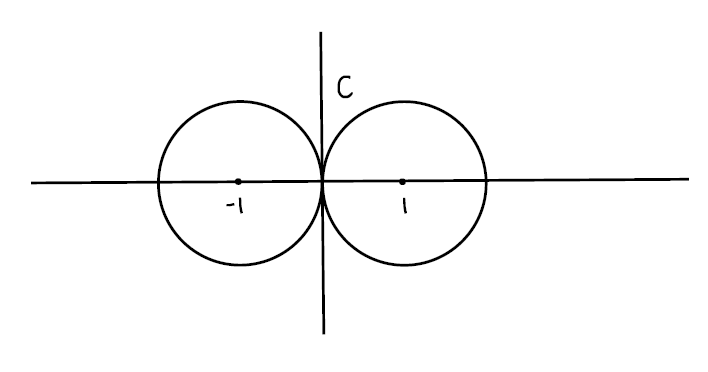
\includegraphics[scale=0.75]{Sections/Illustrations/Example-3.10.3-3-curve.png}
\end{center}
The contour $C$ is not simple but it can be decomposed as a sum of simple closed contours $C = C_1 - C_2$
\begin{center}
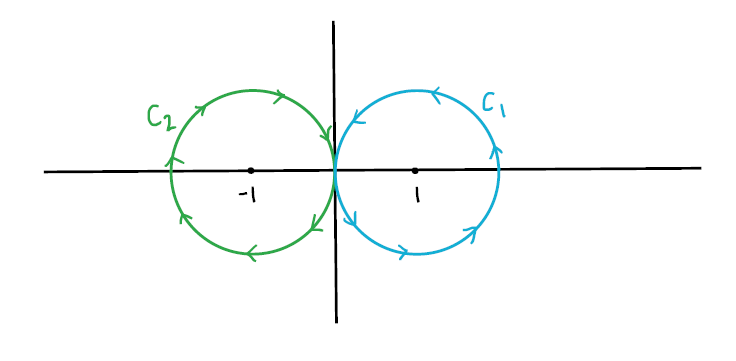
\includegraphics[scale=0.75]{Sections/Illustrations/Example-3.10.3-3-contour.png}
\end{center}
So, 
\[\int_C\, \frac{z^2 + 1}{(z - 1)(z + 1)}\,dz = \int_{C_1}\, \frac{z^2 + 1}{(z - 1)(z + 1)}\,dz - \int_{C_2}\, \frac{z^2 + 1}{(z - 1)(z + 1)}\,dz\]
For $C_1$, consider
\[f(z) = \frac{z^2 + 1}{z + 1},\]
then $f$ is holomorphic on all points on and interior to $C_1$, as they don't include $-1$, and $1$ is in the interior or $C_1$. Therefore by Cauchy's Integral Formula (Theorem \ref{cintform}) we have
\[\int_{C_1}\, \frac{z^2 + 1}{(z - 1)(z + 1)}\,dz = \int_{C_1}\, \frac{f(z)}{z - 1}\,dz = 2\pi i\cdot f(1) = 2\pi i\]
For $C_2$, consider
\[g(z) = \frac{z^2 + 1}{z - 1},\]
then $g$ is holomorphic on all points on and interior to $C_2$, as they don't include $1$, and $-1$ is in the interior or $C_2$. Therefore by Cauchy's Integral Formula (Theorem \ref{cintform}) we have
\[\int_{C_2}\, \frac{z^2 + 1}{(z - 1)(z + 1)}\,dz = \int_{C_2}\, \frac{g(z)}{z + 1}\,dz = 2\pi i\cdot g(-1) = -2\pi i\]
Hence, 
\[\int_C\, \frac{z^2 + 1}{(z - 1)(z + 1)}\,dz = \int_{C_1}\, \frac{z^2 + 1}{(z - 1)(z + 1)}\,dz - \int_{C_2}\, \frac{z^2 + 1}{(z - 1)(z + 1)}\,dz = 2\pi i + 2\pi i = 4\pi i.\]
\end{itemize}
\end{example}

\medskip

\begin{theorem}[Generalised Cauchy's Integral Formula]\label{gencintform}
Let $C$ be a simple closed contour, with positive orientation, and let $f$ be a function that is holomorphic at all points on and interior to $C$. The for any $z_0 \in \mathrm{int}(C)$, we have that $f^{(n)}(z_0)$ exists and
\[f^{(n)}(z_0) = \frac{n!}{2\pi i}\int_C\,\frac{f(z)}{(z - z_0)^{n+1}}\,dz\]
\end{theorem}
\begin{proof}
We prove by induction, with the base case $n = 0$ being just Theorem \ref{cintform}. Assume the statements holds for $n = k$, we need to prove  that
\[f^{(k+1)}(z_0) \coloneqq \lim_{h \to 0}\frac{f^{(k)}(z_0 + h) - f^{(k)}(z_0)}{h} = \frac{(k+1)!}{2\pi i}\int_C\,\frac{f(z)}{(z - z_0)^{(k+1)+1}}\,dz\]
We assume $\abs{h}$ is small enough such that $z + h \in \mathrm{int}(C)$, then by the inductive hypothesis
\begin{align*}
f^{(k)}(z_0 + h) &= \frac{k!}{2\pi i}\int_C\,\frac{f(z)}{(z - (z_0 + h))^{k+1}}\,dz\\[1em]
f^{(k)}(z_0) &= \frac{k!}{2\pi i}\int_C\,\frac{f(z)}{(z - z_0)^{k+1}}\,dz
\end{align*}
Recall the algebraic identity, that for $a,\,b \in \cc$ we have
\[a^{k+1} - b^{k+1} = (a - b)(a^k + a^{k-1}b + \cdots + ab^{k-1} + b^k),\]
We will apply this to $a = \dfrac{1}{z - z_0 - h}$ and $b = \dfrac{1}{z - z_0}$, and we also note $\lim_{h \to 0}a = b$. Then,
\begin{align*}
\lim_{h \to 0}&\,\frac{f^{(k)}(z_0 + h) - f^{(k)}(z_0)}{h}\\[1em]
&= \lim_{h \to 0}\,\frac{k!}{2\pi i}\int_C\,\frac{f(z)}{h}\left(\frac{1}{(z - z_0 - h)^{k+1}} - \frac{1}{(z - z_0)^{k+1}}\right)\,dz\\[1em]
 &= \lim_{h \to 0}\,\frac{k!}{2\pi i}\int_C\,\frac{f(z)}{h}\left(\frac{1}{z - z_0 - h} - \frac{1}{z - z_0}\right)(a^k + a^{k-1}b + \cdots + ab^{k-1} + b^k)\,dz \\[1em]
 &= \lim_{h \to 0}\,\frac{k!}{2\pi i}\int_C\,\frac{f(z)}{h}\left(\frac{h}{(z - z_0 - h)(z - z_0)}\right)(a^k + a^{k-1}b + \cdots + ab^{k-1} + b^k)\,dz%\\[1em]
\end{align*}
\begin{align*}
 \phantom{\lim_{h \to 0}} &= \lim_{h \to 0}\,\frac{k!}{2\pi i}\int_C\,\left(\frac{f(z)}{(z - z_0 - h)(z - z_0)}\right)(a^k + a^{k-1}b + \cdots + ab^{k-1} + b^k)\,dz \\[1em]
 &= \frac{k!}{2\pi i}\int_C\,\lim_{h \to 0}\,\left(\frac{f(z)}{(z - z_0 - h)(z - z_0)}\right)(a^k + a^{k-1}b + \cdots + ab^{k-1} + b^k)\,dz \\[1em]
 &= \frac{k!}{2\pi i}\int_C\,\left(\frac{f(z)}{(z - z_0)^2}\right)(b^k + b^{k-1}b + \cdots + b\cdot b^{k-1} + b^k)\,dz\\[1em]
 &= \frac{k!}{2\pi i}\int_C\,\frac{f(z)}{(z - z_0)^2}\cdot(k+1)\cdot b^k\,dz \\[1em]
 &= \frac{(k+1)!}{2\pi i}\int_C\,\frac{f(z)}{(z - z_0)^2}\cdot\frac{1}{(z - z_0)^k}\,dz \\[1em]
 &= \frac{(k+1)!}{2\pi i}\int_C\,\frac{f(z)}{(z - z_0)^{(k+1)+1}}\,dz 
\end{align*}
Thus we have our result by the principle of mathematical induction. 
\end{proof}

\medskip

\begin{example}
Compute the integral
\[\frac{1}{2\pi i}\int_C\,\frac{(1 + z)^n}{z^{k+1}}\,dz\]
where $C$ is any simple closed positively oriented contour whose interior contains $0$ and $0 \leq k \leq n$.\\
\\
Let $f(z) = (1 + z)^n$, since $f$ is entire, $f$ is holomorphic on all points on and interior to $C$. Since $0$ is in the interior of $C$, then generalised Cauchy's Integral formula (Theorem \ref{gencintform}) gives us
\begin{align*}
\frac{1}{2\pi i}\int_C\,\frac{(1 + z)^n}{z^{k+1}}\,dz &= \frac{1}{k!}\left(\frac{k!}{2\pi i}\int_C\,\frac{(1 + z)^n}{(z - 0)^{k+1}}\,dz\right) = \frac{1}{k!}\cdot f^{(k)}(0)
\end{align*}
We have, 
\[f^{(k)}(z) = n(n-1)\cdots (n-(k-1))(1 + z)^{n-k},\]
and therefore
\[f^{(k)}(0) = n(n-1)\cdots (n-(k-1)) = \frac{n!}{(n-k)!}\]
Hence, 
\[\frac{1}{2\pi i}\int_C\,\frac{(1 + z)^n}{z^{k+1}}\,dz = \frac{1}{k!}\cdot f^{(k)}(0) = \frac{n!}{k!(n-k)!} = \binom{n}{k}\]
\end{example}

\medskip

\begin{theorem}[Derivatives of Holomorphic functions are Holomorphic]\label{holsmooth}
Suppose that $f$ is holomorphic at $z_0 \in \cc$, then for all $n\in \zz_{>0}$, $f^{(n)}$ is also holomorphic at $z_0$. 
\end{theorem}
\begin{proof}
Suppose $f$ is holomorphic at $z_0 \in \cc$. Choose an open disk $D_\epsilon(z_0)$ on which $f$ is differentiable. To conclude $f'$ exists and is holomorphic at $z_0$, it's enough to find a neighbourhood of $z_0$ where $f''(w)$ exists for all $w$ in that neighbourhood. Let $C$ be the positive oriented circle of radius $\epsilon/2$ centered at $z_0$, then $f$ is holomorphic on all points on and interior to $C$. So, by generalised Cauchy's Integral formula (Theorem \ref{gencintform}),
\[f''(w) = \frac{2!}{2\pi i}\int_C\,\frac{f(z)}{(z - w)^3}\,dz\]
for any $w$ in the interior of $C$. Thus, $f'$ is differentiable in the open set $D_{\epsilon/2}(z_0)$, and hence $f'$ is holomorphic at $z_0$. Induction then gives us that $f^{(n)}$ is holomorphic at $z_0$ for any $n\in \zz_{>0}$.
\end{proof}

\medskip

\begin{corollary}
If $f(z) = u(x,y) + iv(x,y)$ is holomorphic at $z = x + iy$, then $u$ and $v$ have continuous partial derivatives of all orders at $(x,y)$. 
\end{corollary}

\medskip

\begin{theorem}[Morera's Theorem]\label{morera}\lecmargin{27}
Suppose $f$ is continuous on a domain $G$. If
\[\int_C\,f(z)\,dz = 0\]
for every closed contour $C \subseteq G$, then $f$ is holomorphic on $G$. 
\end{theorem}
\begin{proof}
By Theorem \ref{FTCoCI}, there exists a holomorphic function $F:G \to \cc$ such that $F'(z) = f(z)$ for all $z \in G$. But by Theorem \ref{holsmooth}, $F'$ is holomorphic on $G$, and therefore so is $f$. 
\end{proof}

\medskip

\begin{remark}
When $G$ is simply connected, Morera's theorem (Theorem \ref{morera}) is just the converse of Cauchy-Goursat Theorem for simply connected domains (Theorem \ref{cgthmsc}).
\end{remark}

\medskip

\begin{theorem}[Cauchy's Inequalities]\label{cauchyineq}
Suppose that $f$ is holomorphic on all points on and interior to $C_R = C_R(z_0)$, a positively oriented circle of radius $R$ centered at some $z_0 \in \cc$. Then,
\[|f^{(n)}(z_0)| \leq \frac{n!}{R^n}\,\max_{z \in C_R(z_0)}\abs{f(z)}\]
\end{theorem}
\begin{proof}
By Theorem \ref{gencintform}, 
\[f^{(n)}(z_0) = \frac{n!}{2\pi i}\int_{C_R}\,\frac{f(z)}{(z - z_0)^{n+1}}\,dz\]
Hence, 
\begin{align*}
|f^{(n)}(z_0)|= \abs{\frac{n!}{2\pi i}\int_{C_R}\,\frac{f(z)}{(z - z_0)^{n+1}}\,dz} &= \frac{n!}{2\pi i}\abs{\int_{C_R}\,\frac{f(z)}{(z - z_0)^{n+1}}\,dz}\\[1em]
&\leq \frac{n!}{2\pi i}\max_{z \in C_R}\,\abs{\frac{f(z)}{(z - z_0)^{n+1}}}\cdot L(C_R)\\[1em]
&= \frac{n!}{2\pi i}\max_{z \in C_R}\,\frac{\abs{f(z)}}{R^{n+1}}\cdot 2\pi R\\[1em]
&= \frac{n!}{R^n}\,\max_{z \in C_R}\abs{f(z)}\\[-2.5em]
\end{align*}
\end{proof}

\bigskip

\subsection{Liouville's Theorem and the Fundamental Theorem of Algebra}
%\begin{mdframed}
%\begin{center}
%{\Large Liouville's Theorem and the Fundamental Theorem of Algebra}
%\end{center}
%\end{mdframed}
As an application, we will prove that every non-constant polynomial with complex coefficients has a root in $\cc$. In the language of algebra, we will provide a proof for the fact that $\cc$ is \emph{algebraically closed}. Thus, the the statement is ``purely algebraic" while no ``purely algebraic" proof exists. The proof relies on the following wonderful theorem. 

\medskip

\begin{theorem}[Liouville's Theorem]\label{liouville}
Every bounded entire function is constant. 
\end{theorem}
\begin{proof}
We show that $f'(z) = 0$ for all $z \in \cc$, then it follows that $f$ is constant since $\cc$ is a domain by Theorem \ref{der0const}.\\
\\
Consider any $z_0 \in \cc$. Since $f$ is bounded, we can find a $M>0$ such that $\abs{f(z)} \leq M$ for all $z \in \cc$. Let $C_R(z_0)$ be a circle of radius $R$ centered at $z_0$, then $f$ is holomorphic at all points on and interior to $C_R(z_0)$. Hence, by Theorem \ref{cauchyineq},
\begin{align*}
\abs{f'(z_0)} &\leq \frac{1}{R}\max_{z \in C_R(z_0)}\abs{f(z)}\\[0.5em]
&\leq \frac{M}{R} \to 0,\ \text{ as } R \to \infty
\end{align*}
Thus $\abs{f'(z_0)} = 0$, giving us $f'(z_0) = 0$. Since $z_0$ was arbitrary, the result follows. 
\end{proof} 

\medskip

\begin{theorem}[Fundamental Theorem of Algebra]
For any polynomial $p(z) = a_0 + a_1z + \cdots + a_nz^n$ where $a_n \neq 0,\ a_i \in \cc$ and $n \geq 1$, there exists an $\alpha \in \cc$ such that $p(\alpha) = 0$. That is, every non-constant polynomial $p(z)$ has at least one root in $\cc$. 
\end{theorem}
\begin{proof}
Suppose otherwise that $p(z)$ has no root in $\cc$, then $p(z) \neq 0$ for every $z \in \cc$. Hence $1/p(z)$ is an entire function. We show that $1/p(z)$ is bounded.\\
\\
For a non-zero $z \in \cc$, consider the complex number
\[w_z \coloneqq \frac{a_0}{z^n} + \frac{a_1}{z^{n-1}} + \cdots + \frac{a_{n-1}}{z}\]
Note that $p(z) = (w_z + a_n)\ z^n$, and by triangle inequality we have
\[\abs{w_z} \leq \frac{\abs{a_0}}{\abs{z}^n} + \frac{\abs{a_1}}{\abs{z}^{n-1}} + \cdots + \frac{\abs{a_{n-1}}}{\abs{z}} = \sum_{k=0}^{n-1}\frac{\abs{a_k}}{\abs{z}^{n-k}}\]
For each $0 \leq k \leq n-1$ we note that $\dfrac{\abs{a_k}}{\abs{z}^{n-k}} \to 0$ as $z \to \infty$.\\[0.5em]
Then, for $\epsilon = \dfrac{\abs{a_n}}{2n} > 0$, we can find an $R > 0$ such that whenever $\abs{z} > R$, we get
\[\frac{\abs{a_k}}{\abs{z}^{n-k}} = \abs{\frac{\abs{a_k}}{\abs{z}^{n-k}} - 0} < \epsilon = \frac{\abs{a_n}}{2n}\]
for any $k = 0,\ldots,n-1$. This then gives us
\[\abs{w_z} \leq \sum_{k=0}^{n-1}\frac{\abs{a_k}}{\abs{z}^{n-k}} < \sum_{k=0}^{n-1}\frac{\abs{a_n}}{2n} = n\cdot \frac{\abs{a_n}}{2n} = \frac{\abs{a_n}}{2}\]
Now, by the reverse triangle inequality we have
\[\abs{a_n + w_z} \geq \abs{\abs{a_n} - \abs{w_z}} > \abs{\abs{a_n} - \frac{\abs{a_n}}{2}} = \frac{\abs{a_n}}{2}\]
Thus, 
\begin{align*}
\abs{p(z)} &= \abs{(w_z + a_n)\ z^n}\\[0.5em]
&= \abs{w_z + a_n}\abs{z^n} > \frac{\abs{a_n}}{2}R^n
\end{align*}
Therefore, for any $z \in \cc$ such that $\abs{z} > R$, we have
\[\abs{\frac{1}{p(z)}} \leq \frac{2}{R^n\abs{a_n}}\]
So, $1/p(z)$ is bounded outside the closed disk $\overline{D}_R(0)$.\\[0.5em]
Now, the closed disk $\overline{D}_R(0)$ is compact (closed and bounded) and $1/p(z)$ is continuous on $\overline{D}_R(0)$. Hence $1/p(z)$ is bounded on $\overline{D}_R(0)$ by Theorem \ref{evt}.\\
\\
Thus, $1/p(z)$ is bounded on all of $\cc$. Hence, by Theorem \ref{liouville}, $1/p(z)$ is constant, and therefore so is $p(z)$. We have arrived a contradiction, since $p(z)$ was non-constant by assumption. 
\end{proof}

\medskip

\begin{lemma}[Maximum Modulus Principle]
Suppose that $\abs{f(z)} \leq \abs{f(z_0)}$ at each point $z$ in a neighbourhood $D_\epsilon(z_0)$ where $f$ is holomorphic. Then $f(z) = f(z_0)$ on $D_\epsilon(z_0)$. That is, if a holomorphic function on an open disk achieves its maximum on it, then it is constant on the open disk.
\end{lemma}
\begin{proof}
Let $z_1 \in D_\epsilon(z_0)$ such that $z_1 \neq z_0$. Set $\rho \coloneqq \abs{z_1 - z_0} > 0$, and consider $C_\rho = C_\rho(z_0)$, the circle of radius $\rho > 0$ centered at $z_0$, which is interior to $D_\epsilon(z_0)$. We parametrise $C_\rho$ as $z(t) = z_0 + \rho e^{it}$ for $0 \leq t \leq 2\pi$.
\begin{center}
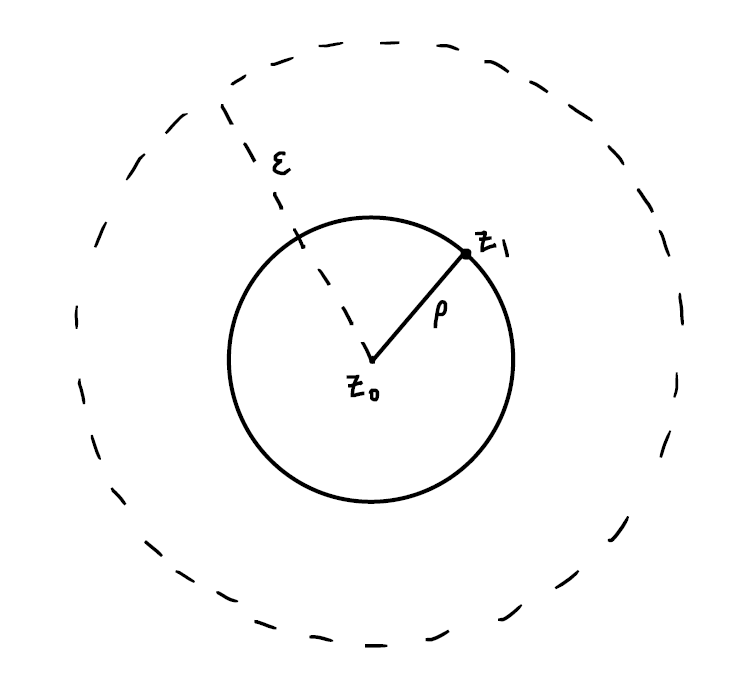
\includegraphics[scale=0.55]{Sections/Illustrations/MMP.png}
\end{center}
By Theorem \ref{cintform},
\begin{align*}
\abs{f(z_0)} = \abs{\frac{1}{2\pi i}\int_{C_\rho}\,\frac{f(z)}{z - z_0}\, dz} &= \frac{1}{2\pi}\abs{\int_{C_\rho}\,\frac{f(z)}{z - z_0}\, dz}\\[1em]
 &= \frac{1}{2\pi}\abs{\int_0^{2\pi}\,\frac{f(z_0 + \rho e^{it})}{\rho e^{it}}\,i\rho e^{it}\ dt}\\[1em]
 &= \frac{1}{2\pi}\abs{\int_0^{2\pi}\,f(z_0 + \rho e^{it})\ dt}\\[1em]
 &\leq \frac{1}{2\pi}\int_0^{2\pi}\,|f(z_0 + \rho e^{it})|\ dt\\[1em]
 &\leq \frac{1}{2\pi}\int_0^{2\pi}\,\abs{f(z_0)}\ dt,\quad \text{by assumption}\\[1em]
 &\leq \abs{f(z_0)}
\end{align*} 
This tells us that
\[\abs{f(z_0)} = \frac{1}{2\pi}\int_0^{2\pi}\,|f(z_0 + \rho e^{it})|\ dt \tag{$\dagger$}\]
Since, $\displaystyle f(z_0) =  \frac{1}{2\pi}\int_0^{2\pi}\,\abs{f(z_0)}\ dt$. Rewriting ($\dagger$), we have
\[\frac{1}{2\pi}\int_0^{2\pi}\, \abs{f(z_0)} - |f(z_0 + \rho e^{it})|\ dt = 0\]
By assumption $\abs{f(z_0)} - |f(z_0 + \rho e^{it})| \geq 0$; suppose $\abs{f(z_0)} - |f(z_0 + \rho e^{it})| > 0$, then necessarily 
\[\frac{1}{2\pi}\int_0^{2\pi}\, \abs{f(z_0)} - |f(z_0 + \rho e^{it})|\ dt > 0\tag{$*$}\]
since the integrand in ($*$) is continuous in the variable $t$, giving us a contradiction. Thus, 
\[\abs{f(z_0)} - |f(z_0 + \rho e^{it})| = 0\]
Therefore $\abs{f(z)} = \abs{f(z_0)}$ for every $z \in C_\rho(z_0)$. Varying the radius $\rho > 0$, we may then obtain $\abs{f(z)} = \abs{f(z_0)}$ for every $z \in D_\epsilon(z_0)$.\\
\\
Thus, $\abs{f}$ is a holomorphic function on $D_\epsilon(z_0)$, and thus by Corollary \ref{absholconst}, we have $f$ is constant on $D_\epsilon(z_0)$ and $f(z) = f(z_0)$ for every $z \in D_\epsilon(z_0)$.
\end{proof}
\newpage

%\section{Lecture 1 (4/03)}
%\input{Lectures/Lecture 1}
%\newpage
%
%\section{Lecture 2 (4/05)}
%\input{Lectures/Lecture 2}
%\newpage
%
%\section{Lecture 3 (4/07)}
%\input{Lectures/Lecture 3}
%\newpage
%
%\section{Lecture 4 (4/10)}
%\input{Lectures/Lecture 4}
%\newpage
%
%\section{Lecture 5 (4/12)}
%\input{Lectures/Lecture 5}
%\newpage
%
%\section{Lecture 6 (4/14)}
%\input{Lectures/Lecture 6}
%\newpage
%
%\section{Lecture 7 (4/17)}
%\input{Lectures/Lecture 7}
%\newpage
%
%\section{Lecture 8 (4/19)}
%\input{Lectures/Lecture 8}
%\newpage
%
%\section{Lecture 9 (4/21)}
%\input{Lectures/Lecture 9}
%\newpage
%
%\section{Lecture 10 (4/24)}
%\input{Lectures/Lecture 10}
%\newpage
%
%\section{Lecture 11 (4/26)}
%\input{Lectures/Lecture 11}
%\newpage
%
%\section{Lecture 12 (4/28)}
%\input{Lectures/Lecture 12}
%\newpage
%
%\section{Lecture 13 (5/01)}
%\input{Lectures/Lecture 13}
%\newpage
%
%\section{Lecture 14 (5/03)}
%\input{Lectures/Lecture 14}
%\newpage
%
%\section{Lecture 15 (5/05)}
%\input{Lectures/Lecture 15}
%\newpage
%
%\section{Lecture 16 (5/08)}
%\input{Lectures/Lecture 16}
%\newpage
%
%\section{Lecture 17 (5/10)}
%\input{Lectures/Lecture 17}
%\newpage
%
%\section{Lecture 18 (5/12)}
%\input{Lectures/Lecture 18}
%\newpage
%
%\section{Lecture 19 (5/15)}
%\input{Lectures/Lecture 19}
%\newpage
%
%\section{Lecture 20 (5/17)}
%\input{Lectures/Lecture 20}
%\newpage
%
%\section{Lecture 21 (5/19)}
%\input{Lectures/Lecture 21}
%\newpage
%
%\section{Lecture 22 (5/22)}
%\input{Lectures/Lecture 22}
%\newpage
%
%\section{Lecture 23 (5/24)}
%\input{Lectures/Lecture 23}
%\newpage
%
%\section{Lecture 24 (5/26)}
%\input{Lectures/Lecture 24}
%\newpage
%
%\section{Lecture 25 (5/31)}
%\input{Lectures/Lecture 25}
%\newpage
%
%\section{Lecture 26 (6/02)}
%\input{Lectures/Lecture 26}
%\newpage
%
%\section{Lecture 27 (6/05)}
%\input{Lectures/Lecture 27}
%\newpage
%
%\section{Lecture 28 (6/07)}
%\input{Lectures/Lecture 28}
%\newpage
%
%\section{Lecture 29 (6/09)}
%\input{Lectures/Lecture 29}
%\newpage

%\section*{References}
%\vspace{0.1in}

\appendix
\section{Problems}
\begin{problem}[]\label{prob 1.1a}
Consider the set of matrices
\[X \coloneqq \setp{\begin{pmatrix}x & -y\\ y & x \end{pmatrix}}{x,y \in \rr}.\]
One can check (and you should if you're unconvinced) straightforwardly that $X$ is closed under matrix addition and matrix multiplication; that is, if $A,B \in X$, then $A+B,\, AB \in X$.
\begin{itemize}[itemsep=1em]
\item[(a)] Let $\cc$ denote the set of complex numbers. Show that the map $\phi: X \to \cc$ defined by 
\[\phi:X \to \cc,\quad \begin{pmatrix}x & -y\\ y & x \end{pmatrix} \mapsto x + iy\]
is a bijection. 
\item[(b)] Let $I = \begin{pmatrix}1 & 0\\ 0 & 1\end{pmatrix}$ be the identity matrix. Consider $A,B \in X$, show that $\phi$ has the following properties.
\begin{itemize}[itemsep=1em]
\item[(i)] $\phi(A+B) = \phi(A)+\phi(B)$
\item[(ii)] $\phi(AB) = \phi(A)\phi(B)$
\item[(iii)] $\phi(I) = 1$
\end{itemize}
\item[(c)] Find a matrix $J$ satisfying $J^2 = -I$ and show that $\phi(J) = i$.
\end{itemize}
\vspace*{0.05in}
\begin{remark}
This indicates that one could very well define $\cc$ to be $X$. The algebraic operations on $\cc$ then seem less artificial, since product and sum of complex numbers correspond to the corresponding operations of matrices. Even taking the inverse and modulus is captured by $X$ as taking inverse and the determinant of matrices. The copy of $\rr$ corresponds to the set of diagonal matrices in $X$. One obtains $X$ by considering the linear operator of multiplying by $x + iy$ on the $\rr$-vector space $\cc$ with basis $1$ and $i$.
\end{remark}
\end{problem}

\medskip

\begin{problem}\label{prob 1.1}
Using the definition of complex multiplication prove that
\[(a,0)\cdot (x,y) = (ax,ay).\]
That is, $a(x + iy) = ax + iay$.
\end{problem}

\vspace*{0.1in}

\begin{problem}\label{prob 1.2}
Consider complex numbers $z_1 = (x_1,y_1) = x_1(1,0) + y_1(0,1)$ and $z_2 = (x_2,y_2) = x_2(1,0) + y_2(0,1)$. Using the identity $(0,1)^2 = (-1,0)$. Prove that \[(x_1(1,0) + y_1(0,1))\cdot (x_2(1,0) + y_2(0,1)) = (x_1x_2 - y_1y_2, x_1y_2 + x_2y_1),\] where the former is computed distributively.
\end{problem}

\newpage
%\medskip

\begin{problem}\label{prob 1.3}
Prove properties (1) - (7) and (9) listed in Proposition \ref{cafield}.
\end{problem}

\medskip

\begin{problem}\label{prob 1.3a}
Prove that if $z_1z_2 = 0$, then $z_1 = 0$ or $z_2 = 0$.
\end{problem}

\medskip

\begin{problem}\label{prob 1.4}
Show that
%\begin{multicols}{2}
\begin{itemize}
\item[(a)] $\Re iz = - \Im z$;
\item[(b)] $\Im iz = \Re z$
\end{itemize}
%\end{multicols}
\end{problem}

\medskip

\begin{problem}\label{prob 1.5}\hfill
\begin{itemize}
\item[(a)] Verify that $z = 1 \pm i$ satisfies the equation \[z^2 - 2z + 2 = 0.\]
\item[(b)] Solve the equation \[z^2 + z + 1 = 0\] for $z = x + iy$ by solving a pair of simultaneous equations in $x$ and $y$.
\end{itemize}
\end{problem}

\medskip

\begin{problem}\label{prob 1.5a}
Let $p(z) = az^2 + bz + c$ be a polynomial with complex coefficients ($a\neq 0$). 
\begin{itemize}
\item[(a)] By completing the square, show that the solution to $p(z) = 0$ is
\[z = \frac{-b \pm \Delta^{1/2}}{2a},\]
where $\Delta \coloneqq b^2 - 4ac$ is called the discriminant.\\[0.5em]
{\footnotesize Remark. There's a subtlety with taking roots that we will address later in class.}
\item[(b)] Consider the polynomial $p(z) = iz^2 -1$
\begin{itemize}
\item[(i)] Compute $\Delta$.
\item[(ii)] For the $\Delta$ obtained in (b), compute $\Delta^{1/2}$ by solving a pair of simultaneous equations in $x$ and $y$ obtained by considering the equation \[x^2 - y^2 + 2ixy = (x + iy)^2 = \Delta.\]
\item[(iii)] Finally, write down the roots of $p(z)$ in the form $u + iv$.
\end{itemize}
\end{itemize}
\end{problem}

\medskip

\begin{problem}\label{prob 1.6}
Suppose $\cc$ had total ordering that extends the ordering on $\rr$, arrive at a contradiction by comparing $i$ and $0$.
\end{problem}

\medskip

\begin{problem}\label{prob 1.7}
Locate the numbers $z_1 + z_2,\, z_1 - z_2$ and $z_1z_2$ in the complex plane when
\begin{multicols}{2}
\begin{itemize}
\item[(a)] $z_1 = 2i,\, z_2 = \dfrac{2}{3} - i$.
\item[(b)] $z_1 = (-3,1),\,z_2 = (1,4)$.
\item[(c)] $z_1 = (-\sqrt{3},1),\,z_2 = (\sqrt{3},0)$.
\item[(d)] $z_1 = x_1 + iy_1,\,z_2 = x_1 - iy_1$.
\end{itemize}
\end{multicols}
\end{problem}

\medskip

\begin{problem}\label{prob 1.8}
Verify that $\sqrt{2}\abs{z} \geq \abs{\Re z} + \abs{\Im z}$.
\end{problem}

\medskip

\begin{problem}\label{prob 1.9}
Let $z_0\neq z_1 \in \cc$ and let $\lambda >0$.
\begin{itemize}[itemsep=1em]
\item[(a)] Show that if $\lambda \neq 1$, then the set of points
\begin{equation*}\label{par}
\abs{z-z_0} = \lambda \abs{z-z_1}\tag{$\bigstar$}
\end{equation*}
is a circle of radius $R = \dfrac{\lambda}{\abs{1-\lambda^2}} \abs{z_0 - z_1}$ centered at $w = \dfrac{z_0 - \lambda^2 z_1}{1-\lambda^2}$.\\[0.5em]
\item[(b)] Show that every circle in the complex plane can be written in the form of (\ref{par}) for some $\lambda >0,\, \lambda \neq 1$ and $z_0 \neq z_1 \in \cc$. 
\item[(c)] If $\lambda = 1$, show that (\ref{par}) defines a line. In fact, argue that the resulting line is perpendicular to and bisects the line segment joining $z_0$ and $z_1$, by producing the equation of this line as a subset of $\rr^2$.
\item[(d)] Characterise points on the real (resp. imaginary) axis using (c). That is, find $z_0 \neq z_1 \in \cc$ such that the points on the real (resp. imaginary) axis satisfy (\ref{par}) for $\lambda = 1$.
\item[(e)] Consider the map \[M(z) = \dfrac{z-3}{1 - 2z}.\] For which values of $c \in \rr$ is the image of the circle $\abs{z - 1} = c$ under $M$ a line? What is the equation of the line when considered as a subset of the plane $\rr^2$?
\end{itemize}
\end{problem}

\medskip

\begin{problem}\label{prob 2.1a}
Prove Proposition \ref{normmult} (1).
\end{problem}

\medskip

\begin{problem}\label{prob 2.1}
Prove the properties, other than (5), listed in Proposition \ref{conjprop}.
\end{problem}

\medskip

\begin{problem}\label{prob 2.2}
Prove that $z$ is either real or pure imaginary if and only if $z^2 = \overline{z}^2$.
\end{problem}

\medskip

\begin{problem}\label{prob 2.3}
Prove that $\abs{z} = 1$ if and only if $\overline{z} = \dfrac{1}{z}$. 
\end{problem}

\medskip

\begin{problem}\label{prob 2.4}
Follow the steps below to give an algebraic derivation of the triangle inequality (Proposition \ref{triangleineq} (a))
\begin{itemize}
\item[(a)] Show that
\[\abs{z_1 + z_2}^2 = (z_1 + z_2)(\overline{z}_1 + \overline{z}_2) = z_1\overline{z}_1 + (z_1\overline{z}_2 + \overline{z_1\overline{z}_2}) + z_2\overline{z}_2.\]
\item[(b)] Argue why
\[z_1\overline{z}_2 + \overline{z_1\overline{z}_2} = 2\Re(z_1\overline{z}_2) \leq 2\abs{z_1}\abs{z_2}.\]
\item[(c)] Use (a) and (b) to obtain $\abs{z_1 + z_2}^2 \leq (\abs{z_1} + \abs{z_2})^2$. Finally note how the triangle inequality follows from this.
\end{itemize}
\end{problem}

\medskip

\begin{problem}\label{prob 2.4a}
Let $z,w \in \cc$. 
\begin{itemize}[itemsep=1em]
\item[(a)] Prove the formula
\[\abs{z+w}^2 = \abs{z}^2 + 2 \Re z\overline{w} + \abs{w}^2\]
\item[(b)] Use (a) to deduce the \emph{parallelogram law}
\[\abs{z+w}^2 + \abs{z-w}^2 = 2\abs{z}^2 + 2\abs{w}^2\]
Give a geometric interpretation of this formula. 
\end{itemize}
\end{problem}

\medskip

\begin{problem}\label{prob 2.5}
Suppose $p$ is a polynomial with \emph{real coefficients}. Prove that
\begin{multicols}{2}
\begin{itemize}
\item[(a)] $\overline{p(z)} = p(\overline{z})$.
\item[(b)] $p(z) = 0$ if and only if $p(\overline{z}) = 0$.
\end{itemize}
\end{multicols}
\end{problem}

\medskip

\begin{problem}\label{prob 2.7}
Find the principal argument $\parg z$ when
\begin{multicols}{2}
\begin{itemize}
\item[(a)] $-i(3 + 3i)^{-1}$.
\item[(b)] $(1 - i\sqrt{3})^6$.
\end{itemize}
\end{multicols}
\end{problem}

\medskip

\begin{problem}\label{prob 3.1}
Prove that 
\[\arg z + \arg w = \setp{(\parg z + \parg w) + 2k\pi}{k \in \zz}\]
Combining this with Proposition \ref{prodarg} we get that $\parg zw = \parg z + \parg w + 2k\pi$ for some $k \in \zz$ such that $-\pi < \parg z + \parg w + 2k\pi \leq \pi$. That is, to find $\parg zw$, just add $\parg z$ and $\parg w$ and then add or subtract a suitable multiple of $2\pi$ to get it between $-\pi$ and $\pi$.
\end{problem}

\medskip

\begin{problem}\label{prob 3.2}
Prove that for any complex number $z$, we have $\parg \overline{z} = \parg z^{-1} = -\parg z$.
\end{problem}

\medskip

\begin{problem}\label{prob 3.3}\hfill
\begin{itemize}
\item[(a)] Show that if $\Re z_1 > 0$ and $\Re z_2 > 0$, then $\parg(z_1z_2) = \parg z_1 + \parg z_2$.
\item[(b)] Show that if $\Re z > 0$, then $\parg(-z) = -\pi + \parg z$ if $\Im z > 0$ or $\parg(-z) = \pi + \parg z$ if $\Im z< 0$.
\item[(c)] Using (a) and (b), find an expression for $\parg zw$ for any non-zero complex numbers $z$ and $w$, in terms of $\parg z,\,\parg w$ and specific multiples of $\pi$.
\end{itemize}
\end{problem}

\medskip

\begin{problem}\label{prob 3.4}
Compute the $6^{\text{th}}$ roots of unity, explicitly. Show that the principal $6^{\text{th}}$ root of unity is $\zeta_6 = -\omega$, where $\omega$ is as in Example \ref{cuberootofunity}.
\end{problem}

\medskip

\begin{problem}\label{prob 3.5}\hfill
\begin{itemize}
\item[(a)] Let $z\in \cc$. Using the principle of mathematical induction, show that the following formula holds for all integers $n\geq 1$
\[1 + z + z^2 + \cdots + z^n = \frac{1-z^{n+1}}{1-z}.\]	
\item[(b)] Use (a) to derive \emph{Lagrange's Trigonometric Identity}.
\[1 + \cos\theta + \cos^2\theta + \cdots + \cos^n\theta = \frac{2\sin((2n+1)\theta/2)}{2\sin(\theta/2)},\quad 0 < \theta < 2\pi.\]
\item[(c)] If $\zeta_1,\ldots,\zeta_n$ are the \emph{distinct} $n^{\text{th}}$ roots of unity, show that, using (a), $\displaystyle \sum_{i=1}^n \zeta_i = 0$.
\item[(d)] We compute the following sum of real numbers
\begin{equation*}\label{trigsum}
\cos \frac{\pi}{7} + \cos \frac{3\pi}{7} + \cos \frac{5\pi}{7} \tag{$\dagger$}
\end{equation*}
\begin{itemize}[itemsep=1em]
\item[(i)] Let $w = e^{\frac{\pi i}{7}}$. What is $\Re w$ and $w^7$? Furthermore, rewrite (\ref{trigsum}) as
\[\Re(w^{a_1} + w^{a_2} + w^{a_3}),\quad \text{for some $0 \leq a_i < 7$.}\]
\item[(ii)] Replacing $z$ by $-z$ in (a), find a formula for \[\dfrac{z^7 + 1}{z + 1}.\]
Use this to deduce an identity involving $w$ and its powers.
\item[(iii)] Using the identity you found in (iii), conclude that 
\[w^{a_1} + w^{a_2} + w^{a_3} = \frac{1}{1-w}\]
where the $a_i$'s are the numbers you found in (ii).
\item[(iv)] Finally compute (\ref{trigsum}).
\end{itemize}
\end{itemize}
\end{problem}

\medskip

\begin{problem}\label{prob 4.1}\hfill
\begin{itemize}
\item[(a)] Recall that a set is open if every point of the set is an interior point. Prove that a set $U \subseteq \cc$ is open if and only if it does not contain any of its boundary points; that is, $\partial U \cap U = \emptyset$. Then deduce that the complement of a closed set is open.
\item[(b)] Prove that an open disk $D_\epsilon(z_0) = \setp{z \in \cc}{\abs{z - z_0} < \epsilon}$ is a domain; that is, a non-empty open and connected subset of $\cc$.
\end{itemize}
\end{problem}

\vspace{0.1in}

\begin{problem}\label{prob 4.2}
Sketch the sets defined by the following constraints and determine whether they are open, closed, or neither; bounded; connected. What are their boundaries?
\begin{multicols}{2}
\begin{itemize}
\item[(a)] $\abs{z + 3} < 2$.
\item[(b)] $\abs{\Im(z)} < 1$.
\item[(c)] $0 < \abs{z - 1} < 2$.
\item[(d)] $\abs{z - 1} + \abs{z + 1} = 2$.
\item[(e)] $\abs{z - 1} + \abs{z + 1} < 3$.
\item[(f)] $\abs{z} \geq \Re(z) + 1$.
\end{itemize}
\end{multicols}
\end{problem}

\vspace{0.1in}

\begin{problem}\label{prob 4.3}
Let $G$ be the set of points $z \in \cc$ satisfying either $z$ is real and $-2 < z < -1$, or $\abs{z} < 1$, or $z = 1$ or $z = 2$.
\begin{itemize}
\item[(a)] Sketch the set $G$, being careful to indicate exactly the points that are in $G$.
\item[(b)] Determine the interior points of $G$.
\item[(c)] Determine the boundary points of $G$.
\item[(d)] Determine the isolated points of $G$.
\item[(e)] $G$ can be written in three diferent ways as the union of two disjoint nonempty disconnected subsets. Describe them.
\end{itemize}
\end{problem}

\medskip

\begin{problem}\label{prob 4.4}
For each of the functions below, describe the domain of definition that is understood.
\begin{multicols}{2}
\begin{itemize}
\item[(a)] $f(z) = \dfrac{1}{1 + z^2}$
\item[(b)] $f(z) = \parg\left(\dfrac{1}{z}\right)$
\item[(c)] $f(z) = \dfrac{z}{z + \overline{z}}$
\item[(d)] $f(z) = \dfrac{1}{1 - \abs{z}^2}$
\end{itemize}
\end{multicols}
\end{problem}

\vspace{0.1in}

\begin{problem}\label{prob 4.5}\hfill
\begin{itemize}
\item[(a)] Write the function $f(z) = z^3 + z + \overline{z} + 1$ in the form 
\[f(z) = u(x, y) + i\,v(x, y).\]
\item[(b)] Suppose that $f(z) = x^2 - y^2 - 2y + i(2x - 2xy)$, where $z = x + iy$. Use Proposition \ref{conjprop} (6) to write $f(z)$ in terms of $z$, and simplify the result.
\item[(c)] Write the function
\[f(z) = z + \frac{1}{z} \quad (z \neq 0)\]
in the form $f(z) = u(r,\theta) + i\,v(r,\theta)$.
\end{itemize}
\end{problem}

\vspace{0.1in}

\begin{problem}\label{prob 4.6}
Let $f : G \to \cc$ be a complex function, and suppose $z_0$ is an accumulation point of $G$. Show that 
\[\lim_{z \to z_0} f(z) = w_0 \quad \text{if and only if} \quad \lim_{z\to z_0}\abs{f(z) - w_0} = 0.\]
Thereby deduce that 
\[\lim_{z \to z_0} \bar{f}(z) = \overline{w}_0 \quad \text{if and only if} \quad \lim_{z \to z_0} f(z) = w_0.\]
\end{problem}

\vspace{0.1in}

\begin{problem}\label{prob 4.7}
Let $f : G \to \cc$ be a complex function, and suppose $z_0$ is an accumulation point of $G$. Show that 
\[\text{if }\lim_{z \to z_0} f(z) = w_0, \quad \text{then }\ \lim_{z\to z_0}\abs{f(z)} = \abs{w_0}.\]
{\footnotesize Hint. Use the reverse triangle inequality.}
\end{problem}

\vspace{0.1in}

\begin{problem}\label{prob 4.8}
Let $f : G \to \cc$ be a complex function, and suppose $z_0$ is an accumulation point of $G$. Writing $h = z - z_0$, show that 
\[\lim_{z \to z_0} f(z) = w_0 \quad \text{if and only if} \quad \lim_{h \to 0}f(z + h) = w_0.\]
\end{problem}

\vspace*{0.1in}

\begin{problem}\label{prob 5.1}
Compute the following limits and prove your claim by using only the $\epsilon$-$\delta$ definition.
\begin{multicols}{2}
\begin{itemize}
\item[(a)] $\displaystyle \lim_{z \to i}\,\overline{z}$
\item[(b)] $\displaystyle \lim_{z \to 1+i}\,z^2$
\item[(c)] $\displaystyle \lim_{z \to 1}\,z^3$
\item[(d)] $\displaystyle \lim_{z \to 1 - i}\,\overline{z}^2 - 1$
\item[(e)] $\displaystyle \lim_{z \to 1}\,z - \overline{z}$
\item[(f)] $\displaystyle \lim_{z \to i}\,\overline{z} + z$
\end{itemize}
\end{multicols}
\end{problem}

\vspace{0.1in}

\begin{problem}\label{prob 5.2}
Evaluate the following limits or explain why they don't exist.
\begin{multicols}{2}
\begin{itemize}
\item[(a)] $\displaystyle \lim_{z\to i}\frac{iz^3 - 1}{z + i}$
\item[(b)] $\displaystyle \lim_{z\to 1-i} (x + i(2x + y))$
\end{itemize}
\end{multicols}
\end{problem}

\vspace{0.1in}

\begin{problem}\label{prob 5.3}
Define
\[f(z) = \frac{x^2y}{x^4 + y^2} \quad \text{where }\  z = x + iy \neq 0.\]
Show that the limits of $f$ at $0$ along all straight lines through the origin exist and are equal, but $\lim_{z \to 0}f(z)$ does not exist.\\[0.5em]
{\footnotesize Hint: Consider the limit along the parabola $y = x^2$.}
\end{problem}

\vspace{0.1in}

\begin{problem}\label{prob 5.4}
Let $M(z) = \dfrac{z - 3}{1 - 2z}$. Prove that
\[\lim_{z\to \infty} M(z) = -\frac{1}{2} \quad \text{and} \quad \lim_{z \to 1/2} M(z) = \infty\]
\end{problem}

\vspace{0.1in}

\begin{problem}\label{prob 5.5}
Let \[M(z) = \dfrac{az + b}{cz + d},\quad ad-bc \neq 0.\] Prove that
\begin{itemize}
\item[(a)] $\displaystyle\lim_{z \to \infty} M(z) = \infty$ if $c = 0$.
\item[(b)] $\displaystyle\lim_{z \to \infty} M(z) = \dfrac{a}{c}$ and $\displaystyle\lim_{z \to -d/c}M(z) = \infty$, if $c \neq 0$.
\end{itemize}
\end{problem}

\medskip

\begin{problem}\label{prob 6.1}
Example \ref{polycts} tells us that polynomials are continuous. 
\begin{itemize}
\item[(a)] Prove that the complex conjugation function $\sigma(z) \coloneqq \overline{z}$ is continuous.
\item[(b)] Prove that a polynomial in $\overline{z}$ is continuous. That is, prove that a polynomial given as
\[p(\overline{z}) = a_n\overline{z}^n + \cdots + a_1\overline{z} + a_0,\quad a_i \in \cc,\ a_n \neq 0\]
is continuous.
\item[(c)] Prove that the following functions are continuous by writing them as a sum or product of polynomials $p(z)$ and $q(\overline{z})$
\begin{itemize}
\item[(i)] $R(z) \coloneqq \Re z$
\item[(ii)] $I(z) \coloneqq \Im z$
\item[(iii)] $N(z) \coloneqq \abs{z}^2$
\end{itemize}
\end{itemize}
\end{problem}

\vspace{0.1in}

\begin{problem}\label{prob 6.2}
Show that the function $f : \cc \to \cc$ given by
\[f(z) = \begin{cases} \dfrac{\overline{z}}{z} & \text{if }z \neq 0\\[1em] 1 & \text{if } z = 0 \end{cases}\]
is continuous on $\cc^*$.
\end{problem}

\vspace{0.1in}

\begin{problem}\label{prob 6.3}
Consider the function \[f : \cc^*\to \cc,\ z \mapsto \frac{1}{z}.\]
Apply the definition of the derivative to give a direct proof that $f'(z) = -\dfrac{1}{z^2}$.
\end{problem}

\vspace{0.1in}

\begin{problem}\label{prob 6.4}
Find the derivative of the function 
\[M(z) \coloneqq \frac{az + b}{cz + d},\quad ad-bc \neq 0.\]
When is $M'(z) = 0$?
\end{problem}

\vspace{0.1in}

\begin{problem}\label{prob 6.5}
Using Example \ref{limnotex} as an inspiration, show that $f'(z)$ does not exist for any $z$ for the functions
\begin{itemize}
\item[(a)] $f(z) = \Re z$
\item[(b)] $f(z) = \Im z$
\end{itemize}
\end{problem}

\vspace{0.1in}

\begin{problem}\label{prob 6.6}
Show that the function $f : \cc \to \cc$ given by
\[f(z) = \begin{cases} \dfrac{\overline{z}^2}{z} & \text{if }z \neq 0\\[1em] 0 & \text{if } z = 0 \end{cases}\]
is not differentiable at $0$.
\end{problem}

\vspace{0.1in}

\begin{problem}\label{prob 6.7}\hfill
\begin{itemize}
\item[(a)] Show that a polynomial of degree $n$, $p(z) = a_0 + a_1z + a_2z^2 + \cdots + a_nz^n$, where $a_n \neq 0$, is differentiable everywhere, with
\[p'(z) = a_1 + 2a_2z + \cdots + na_nz^{n-1}\]
\item[(b)] Furthermore, show that for $p(z)$, as given in (a), we have
\[a_i = \frac{p^{(i)}(0)}{i!}\]
for $i = 0,\ldots,n$. Where $p^{(0)}(z) = p(z)$ and $p^{(i)}(z)$, for $i>0$, is the $i^{\text{th}}$ derivative of $p(z)$.
\end{itemize}
\end{problem}

\vspace{0.1in}

\begin{problem}\label{prob 6.8}
Let $G$ be a domain and $f: G \to \cc$ a function that is differentiable at every point in $G$. Consider the domain
\[G^* = \setp{z \in \cc}{\overline{z} \in G}\]
and the function 
\[f^*:G^* \to \cc,\ z \mapsto \overline{f(\overline{z})}\]
Show that $f^*$ is differentiable at every point in $G^*$.
\end{problem}

\vspace{0.1in}

\begin{problem}\label{prob 6.9}
For each function, determine all points at which the derivative exists. When the derivative exists, find its value. Use Example \ref{normdiffexistence} as an inspiration.
\begin{itemize}
\item[(a)] $f(z) = z + i\overline{z}$
\item[(b)] $g(z) = (z + i\overline{z})^2$
\item[(b)] $h(z) = z\Im z$
\end{itemize}
\end{problem}

\vspace{0.1in}

\begin{problem}\label{prob 6.10}
By definition, a function $f : G \to \cc$ is differentiable at $z_0 \in G$ if the limit
\[f'(z_0) = \lim_{z\to z_0}\frac{f(z) - f(z_0)}{z - z_0}\]
exists. Unpacking the limit definition, we see that $f$ is differentiable at $z_0$ if and only if for every $\epsilon > 0$, there exists a $\delta > 0$ such that
\[\text{if }\ 0 < \abs{z - z_0} < \delta,\quad \text{then }\ \abs{\frac{f(z) - f(z_0)}{z - z_0} - f'(z_0)} < \epsilon.\]
\newpage
By appealing only to the definition, we show that $\sigma : \cc \to \cc$ defined by $\sigma(z) = \overline{z}$ is not differentiable anywhere by completing the following steps.
\begin{itemize}
\item[(i)] Let $z_0 \in \cc$ and assume that $f'(z_0)$ exists. Choose $\delta > 0$ according to the definition using $\epsilon = 1/2$ and write down the resulting statement.
\item[(ii)] Consider $z = z_0 + \delta/2$ and conclude from (a) that $\abs{1 - f'(z_0)} < \epsilon$.
\item[(iii)] Consider $z = z_0 + i\delta/2$ and conclude from (a) that $\abs{1 + f'(z_0)} < \epsilon$.
\item[(iv)] Using the triangle inequality together with (ii) and (iii), obtain a contradiction.
\end{itemize}
\end{problem}

\medskip

\begin{problem}\label{prob 7.1}
Define 
\[f(z) = \begin{cases} 0 & \text{if }\Re(z)\cdot \Im(z) = 0,\\[0.5em] 1 & \text{if } \Re(z)\cdot \Im(z) \neq 0\end{cases}.\]
Show that $f$ satisfies the Cauchy–Riemann equation at $z = 0$, yet $f$ is not diferentiable at $z = 0$.
\end{problem}

\vspace{0.1in}

\begin{problem}\label{prob 7.2}
Show that when $f(z) = x^3 + i(1 - y)^3$, it makes sense to write
\[f'(z) = u_x + iv_x = 3x^2\]
only when $z = i$.
\end{problem}

\vspace{0.1in}

\begin{problem}\label{prob 7.3}
Show that $f'(z)$ does not exist at any point if
\begin{itemize}
\item[(a)] $f(z) = z - \overline{z}$
\item[(b)] $f(z) = 2x + ixy^2$
\end{itemize}
\end{problem}

\vspace{0.1in}

\begin{problem}\label{prob 7.4}
Show that $f'(z)$ and its derivative $f''(z)$ exist everywhere, and find $f''(z)$ when
\begin{itemize}
\item[(a)] $f(z) = iz + 2$
\item[(b)] $f (z) = e^{-x}e^{-iy}$
\end{itemize}
\end{problem}

\vspace{0.1in}

\begin{problem}\label{prob 7.5}
Let $f: G \to \cc$ be a function, such that $G \subseteq \cc^*$, then we can write
\[f(z) = f(x + iy) = u(x,y) + i\,v(x,y)\quad \text{or}\quad f(z) = f(re^{i\theta}) = u(r,\theta) + i\,v(r,\theta)\]
Using the fact that $x = r\cos\theta$ and $y = r\sin\theta$ and the chain rule from calculus, write $u_r$ and $u_\theta$ in terms of $u_x$ and $u_y$. Assuming $f$ is differentiable, rewrite the \ref{creqex}-equations and $f'(z)$ in terms of $u_r$ and $u_\theta$.
\end{problem}

\vspace{0.1in}

\begin{problem}\label{prob 7.6}
Prove that the function
\[f(z) = e^{-\theta}\cos(\ln r) + ie^{-\theta}\sin(\ln r)\]
is differentiable when $r > 0$ and $0 < \theta < 2\pi$, and find $f'(z)$ in terms of $f(z)$.
\end{problem}

\medskip

\begin{problem}\label{prob 8.1}
Let $f = u + iv$ be a complex-valued function defined on an open set $G \subseteq \cc$. Suppose that the first-order partial derivatives of $\Re f = u$ and $\Im f = v$ exist and are continuous on $G$.
\begin{itemize}[itemsep = 1em]
\item[(a)] Recall that if $z = x + iy$, then
\[x = \frac{z + \overline{z}}{2} \quad \text{and} \quad y = \frac{z - \overline{z}}{2i}\]
Treat $f = f(x,y)$ as a function in two real-variables, and \emph{formally} apply the chain rule in Calculus to obtain the expressions
\[\frac{\partial f}{\partial z} = \frac{1}{2}\left(\frac{\partial f}{\partial x} - i\frac{\partial f}{\partial y}\right) \quad \text{and} \quad \frac{\partial f}{\partial \overline{z}} = \frac{1}{2}\left(\frac{\partial f}{\partial x} + i\frac{\partial f}{\partial y}\right)\]
\item[(b)] Define $\dfrac{\partial f}{\partial x} \coloneqq \dfrac{\partial u}{\partial x} + i\dfrac{\partial v}{\partial x}$, and similarly for $\dfrac{\partial f}{\partial y}$.\\[1em] Prove that $f$ is holomorphic on $G$ if and only if $\dfrac{\partial f}{\partial \overline{z}} = 0$.
\item[(c)] 
\begin{itemize}[itemsep=1em]
\item[(i)] If $f$ is holomorphic on $G$, prove that $f'(z) = \dfrac{\partial f}{\partial z}$.
\item[(ii)] The \emph{Jacobian} of $(x,y) \mapsto (u(x,y),v(x,y))$ is the determinant of the matrix
\[\begin{pmatrix}
\dfrac{\partial u}{\partial x} && \dfrac{\partial u}{\partial y}\\[1.5em]
\dfrac{\partial v}{\partial x} && \dfrac{\partial v}{\partial y}
\end{pmatrix}\]
If $f$ is holomorphic on $G$, prove that the Jacobian equals $\abs{f'(z)}^2 \geq 0$.
\end{itemize}
\end{itemize}
\end{problem}

\vspace{0.1in}

\begin{problem}\label{prob 8.2}
Suppose $f$ is entire and can be written as \[f(z) = u(x) + i\,v(y),\] that is, the
real part of $f$ depends only on $x = \Re(z)$ and the imaginary part of $f$ depends only on $y = \Im(z)$.\\[0.5em]
Prove that $f(z) = az + b$ for some $a \in \rr$ and $b \in \cc$.
\end{problem}

\vspace{0.1in}

\begin{problem}\label{prob 8.3}
Suppose $f$ is entire, with real and imaginary parts $u$ and $v$ satisfying
\[u(x, y)\, v(x, y) = 3\]
for all $z = x + i y$. Show that $f$ is constant.
\end{problem}

\vspace{0.1in}

\begin{problem}\label{prob 8.4}
Prove that, if $G \subseteq \cc$ is a domain and $f : G \to \cc$ is a complex-valued function with $f''(z)$ defined and equal to $0$ for all $z \in G$, then $f(z) = az + b$ for some $a, b \in \cc$. 
\end{problem}

\vspace{0.1in}

\begin{problem}\label{prob 8.5}
Show that
\begin{itemize}
\item[(a)] $\exp(2 \pm 3\pi i) = -e^2$
\item[(b)] $\exp\left(\dfrac{2 + \pi}{4}\right) = \sqrt{\dfrac{e}{2}}(1 + i)$
\item[(c)] $\exp(z + \pi i) = -\exp z$.
\end{itemize}
\end{problem}

\vspace{0.1in}

\begin{problem}\label{prob 8.6}
Prove that
\begin{itemize}
\item[(a)] $f(z) = \exp\overline{z}$ is nowhere holomorphic.
\item[(b)] $f(z) = \exp z^2$ is entire. What is its derivative?
\end{itemize}
\end{problem}

\vspace{0.1in}

\begin{problem}\label{prob 8.7}
Show that
\begin{itemize}
\item[(a)] $\abs{\exp(2z + i) + exp(iz^2)} \leq e^{2x} + e^{-2xy}$.
\item[(b)] $\abs{\exp(z^2)} \leq \exp(\abs{z}^2)$.
\item[(c)] $\abs{\exp(-2z)} < 1$ if and only if $\Re z > 0$.
\end{itemize}
\end{problem}

\vspace{0.1in}

\begin{problem}\label{prob 8.8}
Find all values of $z$ such that
\begin{itemize}
\item[(a)] $\exp z = -2$
\item[(b)] $\exp z = 1 + i\sqrt{3}$
\item[(c)] $\exp(2z - 1) = 1$.
\end{itemize}
\end{problem}

\vspace{0.1in}

\begin{problem}\label{prob 8.9}
Find all solutions to the equation $e^{2z} - 2ie^z = 1$.
\end{problem}

\vspace{0.1in}

\begin{problem}\label{prob 8.10}
Let $G \subseteq \cc^*$ be an open set and let $f$ be a function that is continuous on $G$ with the property
\[e^{f(z)} = z,\quad z \in G.\]
Show that $f$ is holomorphic on $G$.
\begin{remark}
This shows that a \emph{continuously} defined logarithm on an open set is immediately holomorphic.
\end{remark}
\end{problem}

\medskip

\begin{problem}\label{prob 9.1}
Find the all possible values of
\begin{multicols}{2}
\begin{itemize}
\item[(a)] $\log(-5)$
\item[(b)] $\log(-2 + 2i)$
\item[(c)] $\log(\sqrt{2} + i\sqrt{6})$
\item[(d)] $\log(-ei)$
\item[(e)] $\log(1 + i)$
\item[(f)] $\log(-\sqrt{3} + i)$
\end{itemize}
\end{multicols}
\end{problem}

\vspace{0.1in}

\begin{problem}\label{prob 9.2}
Compute
\begin{multicols}{2}
\begin{itemize}
\item[(a)] $\plog(6-6i)$
\item[(b)] $\plog(-e^2)$
\item[(c)] $\plog(-12 + 5i)$
\item[(d)] $\plog((1 + i\sqrt{3})^5)$
\item[(e)] $\plog(3 - 4i)$
\item[(f)] $\plog((1+i)^4)$
\end{itemize}
\end{multicols}
\end{problem}

\vspace{0.1in}

\begin{problem}\label{prob 9.3}\hfill
\begin{itemize}
\item[(a)] Show that if $\Re z_1 > 0$ and $\Re z_2 > 0$, then
\[\plog(z_1z_2) = \plog z_1 + \plog z_2.\]
\item[(b)] Show that for any two non-zero complex numbers $z_1$ and $z_2$,
\[\plog(z_1z_2) = \plog z_1 + \plog z_2 + 2N\pi i,\]
where $N \in \set{0,\pm 1}$.
\end{itemize}
\end{problem}

\vspace{0.1in}

\begin{problem}\label{prob 9.4}
Example \ref{logcalc} (4) tells us that it's not necessarily true that $\log z^n = n\log z$, for $n \in \zz_{>0}$.\\[0.5em]
Writing $z = re^{i\parg z}$, show that, where $n \in \zz_{>0}$
\[\log(z^{1/n}) = \frac{1}{n}\ln r + i\left(\frac{\parg z + 2(pn + k)\pi}{n}\right),\quad k = 0,\ldots,n-1.\]
Now, after writing 
\[\frac{1}{n}\log z = \frac{1}{n}\ln r + i\left(\frac{\parg z + 2qz}{n}\right),\quad q \in \zz,\]
show that we have equality of sets
\[\log(z^{1/n}) = \frac{1}{n}\log z\]
\end{problem}

\vspace{0.1in}

\begin{problem}\label{prob 9.5}
Find a domain in which the given function $f$ is holomorphic; then find the derivative $f'$.
\begin{itemize}
\item[(a)] $f(z) = 3z^2 - e^{2iz} + i\plog z$
\item[(b)] $f(z) = (z + 1)\plog z$
\item[(c)] $f(z) = \dfrac{\plog(2z-i)}{z^2 + 1}$
\item[(d)] $f(z) = \plog(z^2 + 1)$
\end{itemize}
\end{problem}

\medskip

\begin{problem}\label{prob 10.1}
Find the all possible values of
\begin{multicols}{2}
\begin{itemize}
\item[(a)] $(-1)^{3i}$
\item[(b)] $3^{2i/\pi}$
\item[(c)] $(1 + i)^{1-i}$
\item[(d)] $(1+i\sqrt{3})^i$
\item[(e)] $(-i)^i$
\item[(f)] $(ei)^{\sqrt{2}}$
\item[(g)] $(-1)^{1/\pi}$
\item[(h)] $i^{i/\pi}$
\end{itemize}
\end{multicols}
\end{problem}

\vspace{0.1in}

\begin{problem}\label{prob 10.2}
Compute the principal value of the given complex powers.
\begin{multicols}{2}
\begin{itemize}
\item[(a)] $(-1)^{3i}$
\item[(b)] $3^{2i/\pi}$
\item[(c)] $2^{4i}$
\item[(d)] $(1+i\sqrt{3})^{3i}$
\item[(e)] $i^{i/\pi}$
\item[(f)] $(1 + i)^{2 - i}$
\item[(g)] $\left(\dfrac{e}{2}(-1-i\sqrt{3})\right)^{3\pi i}$
\item[(h)] $(1 - i)^{4i}$
\end{itemize}
\end{multicols}
\end{problem}

\vspace{0.1in}

\begin{problem}\label{prob 10.3}\hfill
\begin{itemize}
\item[(a)] Verify that $(z^\alpha)^n = z^{n\alpha}$ for $z \neq 0$ and $n \in \zz$.
\item[(b)] Find a counterexample to the statement: $(z^{\alpha})^\beta = z^{\alpha\beta}$, where $z \neq 0$ and $\alpha,\beta \in \cc$.
\end{itemize}
\end{problem}

\vspace{0.1in}

\begin{problem}\label{prob 10.4}
Let $z^\alpha$ represent the principal value of the complex power. Find the derivative of the given function at the given point.
\begin{multicols}{2}
\begin{itemize}
\item[(a)] $z^{3/2};\quad z = 1 + i$
\item[(b)] $z^{1 + i};\quad z = 1 + i\sqrt{3}$
\item[(c)] $z^{2i};\quad z = i$
\item[(d)] $z^{\sqrt{2}};\quad z = -i$
\end{itemize}
\end{multicols}
\end{problem}

\vspace{0.1in}

\begin{problem}\label{prob 10.5}
Let $z \in \cc$.
\begin{itemize}
\item[(a)] Prove that $|1^{z}|$ is single-valued if and only if $\Im z = 0$.
\item[(b)] Find a necessary and sufficient condition for $|i^{iz}|$ to be single-valued.
\item[(c)] Find a counterexample to the statement: $1^z$ is single-valued if and only if $\Im z = 0$.
\end{itemize}
\end{problem}

\vspace{0.1in}

\begin{problem}\label{prob 10.6}
Express the value of the given trigonometric function in the form $x + iy$.
\begin{multicols}{2}
\begin{itemize}
\item[(a)] $\sin(4i)$
\item[(b)] $\cos(-3i)$
\item[(c)] $\cos(2-4i)$
\item[(d)] $\sin\left(\dfrac{\pi}{4} + i\right)$
\item[(e)] $\tan(2i)$
\item[(f)] $\cot(\pi + 2i)$
\item[(g)] $\sec\left(\dfrac{\pi}{2} - i\right)$
\item[(h)] $\csc(1 + i)$
\end{itemize}
\end{multicols}
\end{problem}

\vspace{0.1in}

\begin{problem}\label{prob 10.7}
Find all complex values $z$ satisfying the given equation.
\begin{multicols}{2}
\begin{itemize}
\item[(a)] $\sin z = i$
\item[(b)] $\cos z = 4$
\item[(c)] $\sin z = \cos z$
\item[(d)] $\cos z = i\,\sin z$
\end{itemize}
\end{multicols}
\end{problem}

\vspace{0.1in}

\begin{problem}\label{prob 10.8}
Prove the properties stated in Discussion \ref{trigid}.
\end{problem}

\vspace{0.1in}

\begin{problem}\label{prob 10.9}\hfill
\begin{itemize}
\item[(a)] Prove that $\overline{\cos z} = \cos\overline{z}$.
\item[(b)] What is $\Re \cos z$ and $\Im \cos z$?
\item[(c)] Using the identity $e^{iz} = \cos z + i\sin z$, prove $\overline{\sin z} = \sin\overline{z}$ and find $\Re \sin z$ and $\Im \sin z$. 
\end{itemize}
\end{problem}
\newpage

\nocite{brown2009complex}
\nocite{complex-notes}
\bibliographystyle{amsalpha}
\bibliography{citations.bib}
%
\vspace*{5em}
%
%\thispagestyle{empty}
\centering
\hrule
%\vspace{0.5in}
%\textsc{\LARGE The End}
%\vspace*{\fill}
%\begin{center}
%\emph{Number is the commanding and self-begotten container of the eternal duration of mundane concerns.}
%\end{center}
%\vspace*{-1em}
%\hfill {\footnotesize -- Philolaus, as quoted by Aristotle, \textsl{Metaphysics}}\\[2em]
%\includegraphics[scale=0.25]{Christopher-Farr-Editions-Josef-Albers-Many-Faces-of-Red.jpg}
%\vspace*{\fill}

\end{document}